\documentclass[10pt,a4paper]{report}
\usepackage{amsthm, amsfonts, amsmath, amssymb, mathtools}
\usepackage{algorithm, algpseudocode, listings}
\usepackage{sectsty, csquotes, xcolor, xspace}
\usepackage{graphicx, tabularx}
\usepackage[hidelinks]{hyperref}
\usepackage[capitalise]{cleveref}
\usepackage[inline]{enumitem}
\usepackage[english]{babel}
\usepackage{libertinus}
\usepackage{biblatex}

\theoremstyle{plain}
\newtheorem{theorem}{Theorem}
\newtheorem{lemma}{Lemma}

\theoremstyle{definition}
\newtheorem{definition}{Definition}
\newtheorem{example}{Example}

\theoremstyle{remark}
\newtheorem*{note}{Note}
\newtheorem*{remark}{Remark}

\newcommand{\ALC}{\ensuremath{\texorpdfstring{\mathcal{ALC}}{ALC}}\xspace}
\newcommand{\SROIQ}{\ensuremath{\texorpdfstring{\mathcal{SROIQ}}{SROIQ}}\xspace}
\newcommand{\ALCHOIQ}{\ensuremath{\texorpdfstring{\mathcal{ALCHOIQ}}{ALCHOIQ}}\xspace}
\newcommand{\ALCH}{\ensuremath{\texorpdfstring{\mathcal{ALCH}}{ALCH}}\xspace}

\newcommand{\Lmc}{\ensuremath{\mathcal{L}}\xspace}
\newcommand{\Imc}{\ensuremath{\mathcal{I}}\xspace}
\newcommand{\Tmc}{\ensuremath{\mathcal{T}}\xspace}
\newcommand{\Amc}{\ensuremath{\mathcal{A}}\xspace}
\newcommand{\Rmc}{\ensuremath{\mathcal{R}}\xspace}
\newcommand{\Omc}{\ensuremath{\mathcal{O}}\xspace}
\newcommand{\Omcref}{\ensuremath{{\mathcal{O}^\textnormal{ref}}}\xspace}
\newcommand{\Omcfull}{\ensuremath{{\mathcal{O}^\textnormal{full}}}\xspace}

\newcommand{\Inf}{{\ensuremath{\mathsf{Inf}}}\xspace}
\newcommand{\sub}{{\ensuremath{\mathsf{sub}}}\xspace}
\newcommand{\qual}{{\ensuremath{\mathsf{IIC}}}\xspace}
\newcommand{\UpC}{{\ensuremath{\mathsf{UpCover}}}\xspace}
\newcommand{\DownC}{{\ensuremath{\mathsf{DownCover}}}\xspace}
\newcommand{\inv}{\ensuremath{\mathit{inv}}\xspace}
\newcommand{\refine}{\ensuremath{\mathop{\uparrow}}\xspace}
\newcommand{\corefine}{\ensuremath{\mathop{\downarrow}}\xspace}

\newcommand{\disjoint}{\ensuremath{\mathit{disjoint}}\xspace}
\newcommand{\self}{\ensuremath{\mathit{Self}}\xspace}
\newcommand{\less}[2]{\ensuremath{\leq #1~#2}\xspace}
\newcommand{\more}[2]{\ensuremath{\geq #1~#2}\xspace}
\newcommand{\nominal}[1]{\ensuremath{\{#1\}}\xspace}

\addbibresource{biblio.bib}

\allowdisplaybreaks
\setcounter{tocdepth}{1}
\chapternumberfont{\LARGE}
\chaptertitlefont{\huge}
\interfootnotelinepenalty=10000

\title{Knowledge Refinement in Expressive Description Logics}
\author{Roland Bernard}
\date{July 2023}

\makeatletter
\def\maketitle{
    \begin{tabular}{ll}
        \multicolumn{2}{r}{
\includegraphics[width=0.5\linewidth]{resources/unibz-logo.png}} \\
        \vspace*{40mm} \\
        \multicolumn{2}{l}{\raggedright Bachelor Thesis} \\
        \vspace*{1mm} \\
        \multicolumn{2}{p{\linewidth}}{\raggedright \huge \bf \@title} \\
        \vspace*{30mm} \\
        Candidate   & \@author \\
        \vspace*{5mm} \\
        Supervisors & Oliver Kutz \\
                    & Nicolas Troquard \\
        \vspace*{20mm} \\
        \multicolumn{2}{p{\linewidth}}{\@date}
    \end{tabular}
}

\begin{document}

\maketitle

\begin{abstract}
    The field of ontology engineering plays a crucial role in knowledge representation and has gained significant attention in recent years in many domains, such as medicine and biology. The introduction of the Web Ontology Language as a W3C recommendation has further enabled use cases for ontology engineering in the context of the semantic web. With the growing size and complexity of these ontologies, however, they become more susceptible to bugs, and it becomes harder to debug defects. Moreover, in the context of the semantic web, automatic approaches to debugging ontologies are required for the combination of knowledge derived from conflicting sources. Axiom weakening is a technique that allows for a fine-grained repair of inconsistent ontologies. Its main advantage is that it repairs ontologies by making axioms less restrictive rather than by deleting them, employing refinement operators. Building on previously introduced axiom weakening for \ALC, this thesis presents an extension to the axiom weakening operator to deal with $\SROIQ$, the expressive and decidable description logic underlying OWL 2 DL. The main problem here is to ensure that the global constraints of \SROIQ are preserved in the weakening process, as not every weaker axiom can be inserted into an ontology without compromising them. A basic regularity-preserving weakening approach for \SROIQ is presented, and some alternatives are discussed. Further, the thesis briefly describes a prototype implementation and presents the results of basic experimental evaluations. Additionally, the implementation of the presented axiom weakening techniques as a plugin for the popular ontology editor, Protégé, is discussed.

\end{abstract}

\tableofcontents

\begingroup
\renewcommand{\abstractname}{Acknowledgements}
\begin{abstract}
    \blackout{
I would like to thank Oliver Kutz and Nicolas Troquard for their invaluable guidance and support throughout the creation of this thesis. Their insightful suggestions and feedback have been instrumental in shaping the direction of this work. I am particularly grateful for their proposal of the topic and their assistance in producing a paper, which provided me with invaluable exposure to the research community.

I would also like to extend my appreciation to my fellow students. Their motivation and willingness to exchange ideas have enriched my experience and contributed to the development of this thesis.

Furthermore, I would like to thank my parents and family for their support, belief in my abilities, and constant encouragement throughout my studies. I am grateful for their understanding and patience.

Finally, I would like to acknowledge the contributions of all the individuals whose work has been utilized in this thesis. Their research, publications, and other works in their respective fields have provided the foundation upon which this thesis is built.
}

\end{abstract}
\endgroup

\chapter{Introduction} \label{introduction}


The field of ontologies plays a crucial role in knowledge representation and has gained significant attention in recent years in many domains, such as in biology and medicine. The introduction of the Web Ontology Language as a World Wide Web Consortium (W3C) recommendation has further grown the ecosystem and enabled use cases for ontology engineering in the context of the semantic web.

Ontologies provide a structured and formalized way to represent knowledge about particular domains and facilitate automatic reasoning and knowledge sharing. Nevertheless, the development and maintenance of ontologies is not without challenges. With the growing size and complexity of these ontologies, they become more susceptible to bugs, and it becomes harder to debug these defects. Furthermore, in the context of the semantic web, automatic approaches to correcting ontologies are needed for the combination of conflicting knowledge derived from independent sources.

The \SROIQ Description Logic is a very expressive variant of the Description Logics family, which can serve as the logical basis for representing knowledge in ontologies. It is also the foundation for the Web Ontology Language, a standardized language for representing ontologies on the web, enabling the creation of machine-readable ontologies. In both of these systems, ontologies are sets of axioms, and each axiom is a statement encoding some knowledge about the domain. \SROIQ extends upon basic description logics like \ALC with additional features such as complex role hierarchies, role disjointness axioms, and transitive roles. This expressive power allows for modelling complex domains with rich relationships and constraints. This expressivity, however, comes at the cost of requiring some global restrictions that must be followed in order to ensure the decidability of the logic.

Many approaches to repairing inconsistent ontologies amount to identifying problematic axioms and then removing them (e.g., ~\cite{schlobach2003non,kalyanpur2005debugging,kalyanpur2006repairing,BaPS07}). Whilst this approach is obviously sufficient to guarantee that the obtained ontology is consistent, it tends to lead to information loss as a secondary effect, as outlined in detail in related works \cite{troquard2018repairing,confalonieri2020towards}. 
Axiom weakening has been proposed as a solution for fine-grained repair to inconsistent ontologies. In these approaches, the information loss is reduced by weakening the inferential power of an axiom rather than by deleting it entirely \cite{du2014practical,AMAI-2018,baader2018making,troquard2018repairing,confalonieri2020towards}. 
%
In \cite{troquard2018repairing}, axiom weakening using refinement operators has been described for \ALC and experimentally evaluated, showing that axiom weakening is able to retain more information than deletion. In \cite{confalonieri2020towards}, axiom weakening is extended to include many aspects of \SROIQ, notably omitting, however, the weakening of RBox axioms.

This thesis aims to explore the topic of ontology repair, specifically focusing on axiom weakening in the context of the \SROIQ Description Logic and the Web Ontology Language. It extends upon the previous work on axiom weakening in description logics by extending the underlying basic principles to the logic \SROIQ, including also the possibility of weakening role inclusion axioms and disjoint role axioms. The thesis examines the challenges and difficulties that arise when applying axiom weakening to these more expressive description logics, and covers a number of scenarios where weakening can affect regularity of \SROIQ RBoxes. Further, a framework where these problems can be prevented is proposed.

The implementation of the proposed algorithms will be discussed. Next to a prototype implementation used primarily for running the experimental evaluation, a plugin for the popular ontology editor, Protégé, has been realized. The thesis presents some details of the implementation process and discusses the integration of axiom weakening functionalities into the Protégé tool.

Additionally, by implementing the proposed refinement and weakening operators it becomes possible to perform experimental evaluation, also on ontologies using the more expressive features of \SROIQ. The quality of repairs achieved through axiom weakening is assessed, and the results reaffirm the findings of \cite{troquard2018repairing} for the case of \SROIQ, namely that weakening may significantly outperform deletion. Additionally, the thesis explores the impact of caching in cover computations and evaluates the performance in terms of reasoner calls and execution time.

Finally, the thesis concludes with a summary of the findings, their implications, and possible directions for future research. By addressing some of the challenges related to axiom weakening in the \SROIQ Description Logic, this research aims to contribute to the field of ontology engineering and inspire further research into axiom weakening and ontology repair.


\chapter{Background and Related Work} \label{background}


\section{The \texorpdfstring{$\SROIQ$}{SROIQ} Description Logic} \label{sroiq-def}

% Introduce what description logcs are 
Formally, an ontology is a set of statements expressed in an appropriate logical language and with the purpose of describing a specific domain of interest. While ontologies can be represented using a number of different formalisms, for the use in automated reasoning a trade-off must be made between expressivity and practicality. For example, \emph{first-order logic} (FOL) is more expressive than propositional logic, but this added expressivity comes at the cost of decidability. In addition to decidability, scalability must also be considered in the choice and design of the used representation of the knowledge.

\emph{Description logics} (DL) are often used for building ontologies. They include a family of related knowledge representation languages and are often fragments of FOL\footnote{While DLs are fragments of FOL in the sense that for every ontology in a given DL, there exists a FOL theory that has the same models, the syntax used by DLs is different from the syntax used in FOL, and as such a DL axiom is not a valid FOL sentence.} with equality, as is the case with the DL $\SROIQ$ which is the main focus of this work. DLs are almost always designed to be decidable, and generally offer a favourable trade-off between expressivity and complexity of reasoning tasks. Different DLs have been developed for different applications, and allow for varying levels of expressivity.

This section will briefly introduce the DL $\SROIQ$ \cite{horrocks2006even, rudolph2011foundations, baader_horrocks_lutz_sattler_2017}. A more detailed description, including more explanations and examples, can be found in \cref{sroiq-appendix}.

\subsection{The Syntax of \SROIQ} \label{sroiq-syntax}

% describe the SROIQ syntax
% describe roles and concepts
The syntax of \SROIQ is based on a \emph{vocabulary} of three finite disjoint sets $N_C$, $N_R$, $N_I$ of, respectively, \emph{concept names}, \emph{role names}, and \emph{individual names}. The sets of, respectively, \SROIQ  \emph{roles} and \SROIQ \emph{concepts} are generated by the following grammar.
\begin{alignat*}{2}
  R, S &::={} && U \mid r \mid r^{-} \enspace,\\
  C &::= && \bot \mid \top \mid A \mid \neg C \mid C \sqcap C \mid C \sqcup C \mid \forall R.C \mid \exists R.C \mid \\ 
  &&& \more n S.C \mid \less n S.C \mid \exists S.\self \mid \nominal a \enspace,
\end{alignat*}
where $A \in N_C$ is a concept name, $r \in N_R$ is a role name, $a \in N_I$ is an individual name and $n \in \mathbb{N}_0$ is a non-negative integer. 
%
$U$ is the universal role. $S$ is a \emph{simple role} in the RBox $\Rmc$ (see below). In the following, $\Lmc(N_C, N_R, N_I)$ and $\Lmc(N_R) = N_R \cup \{U\} \cup \{r^- \mid r \in N_R\}$ denote, respectively, the set of concepts and roles that can be built over $N_C$, $N_R$, and $N_I$ in \SROIQ.

We next define the notions of TBox, ABox, and (regular) RBox, of complex role inclusions, and of (non-)simple roles:
% describe the TBox, ABox and RBox statements
A \emph{TBox} $\Tmc$ is a finite set of \emph{concept inclusions} (GCIs) of the form $C \sqsubseteq D$ where $C$ and $D$ are concepts. The TBox is used to store terminological knowledge concerning the relationship between concepts. 
%
An \emph{ABox} $\Amc$ is a finite set of statements of the form $C(a)$, $R(a,b)$, $\lnot R (a,b)$, $a = b$, and $a \not= b$, where $C$ is a concept, $R$ is a role and $a$ and $b$ are individual names. The ABox expresses knowledge regarding individuals in the domain. 
%
An \emph{RBox} $\Rmc$ is a finite set of \emph{role inclusions} (RIAs) of the form $R_1 \circ \cdots \circ R_n \sqsubseteq R$, and disjoint role axioms $\disjoint(S_1, S_2)$ where $R$, $R_1$, $\dots$, $R_n$, $S_1$, and $S_2$ are roles. $S_1$ and $S_2$ are simple (defined next) in the RBox $\Rmc$. The special case of $n = 1$ is a \emph{simple role inclusion}, while we call the cases where $n > 1$ \emph{complex role inclusions}. The RBox represents knowledge about the relationships between roles.

% describe simple and complex roles since it is relevant
The set of \emph{non-simple} roles in $\Rmc$ is the smallest set such that: $U$ is non-simple; any role $R$ that appears as the super role of a complex RIA $R_1 \circ \cdots \circ R_n \sqsubseteq R$ where $n > 1$ is non-simple; any role $R$ that appears on the right-hand side of a simple RIA $S \sqsubseteq R$ where $S$ is non-simple, is also non-simple; and a role $r$ is non-simple if and only if $r^-$ is non-simple.
All other roles are \emph{simple}.

% describe regularity since it is relevant
For convenience, let us define the function $\inv(R)$ such that $\inv(U) = U$, $\inv(r) = r^-$, and $\inv(r^-) = r$ for all role names $r \in N_R$. 
%
An RBox $\Rmc$ is \emph{regular} if there exists a preorder $\preceq$, i.e., a transitive and reflexive relation, over the set of roles appearing in $\Rmc$, such that $R \preceq S \iff \inv(R) \preceq S$, are of the forms:
$\inv(R) \sqsubseteq R$,
$R \circ R \sqsubseteq R$,
$S \sqsubseteq R$, $R \circ S_1 \circ \cdots \circ S_n \sqsubseteq R$,
$S_1 \circ \cdots \circ S_n \circ R \sqsubseteq R$, or
$S_1 \circ \cdots \circ S_n \sqsubseteq R$,
where $n > 1$ and $R$, $S$, $S_1, \cdots, S_n$ are roles such that $S \preceq R$, $S_i \preceq R$, and $R \not\preceq S_i$ for $i = 1, \dots, n$. This regularity restriction has been chosen to align with the implementation of the OWL 2 DL \cite{motik2012ontology} profile checker in the OWL API \cite{horridge2011owl}.

% TODO argue for my version of regularity

\begin{definition}
A \SROIQ  ontology $\Omc = \Tmc \cup \Amc \cup \Rmc$ consists of a TBox $\Tmc$, an ABox $\Amc$, and a RBox $\Rmc$ in the language of \SROIQ, and where the RBox $\Rmc$ is regular.
\end{definition}

\subsection{The Semantics of \SROIQ} \label{sroiq-semantics}

% describe the semantics
% whats a interpretation, when is it a model
The semantics of \SROIQ is defined using \emph{interpretations} $I = \langle \Delta^I, \cdot^I \rangle$, where $\Delta^I$ is a non-empty \emph{domain} and $\cdot^I$ is a function associating to each individual name $a$ an element of the domain $a^I \in \Delta^I$, to each concept $C$ a subset of the domain $C^I \subseteq \Delta^I$, and to each role $R$ a binary relation on the domain $R^I \subseteq \Delta^I \times \Delta^I$. The interpretation function $\cdot^I$ is extended to the interpretation of complex roles and concepts, such that
\begin{align*}
  U^I &= \Delta^I \times \Delta^I \enspace, &
  \top^I &= \Delta^I \enspace, &
  \bot^I &= \emptyset \enspace, &
  \nominal{a}^I &= \{ a^I \} \enspace,
\end{align*}
\vspace{-9mm}
\begin{align*}
  (\lnot C)^I &= \Delta^I \setminus C^I \enspace, &
  (C \sqcap D)^I &= C^I \cap D^I \enspace, &
  (C \sqcup D)^I &= C^I \cup D^I \enspace,
\end{align*} 
\vspace{-9mm}
\begin{align*}
  (r^-)^I &= \{ \langle \gamma_2, \gamma_1 \rangle \mid \langle \gamma_1, \gamma_2 \rangle \in r^I \} \enspace, \\
  (\forall R.C)^I &= \{ \gamma \in \Delta^I \mid \forall \gamma' \in \Delta^I : \langle \gamma, \gamma' \rangle \in R^I \implies \gamma' \in C^I \} \enspace, \\
  (\exists R.C)^I &= \{ \gamma \in \Delta^I \mid \exists \gamma' \in \Delta^I : \langle \gamma, \gamma' \rangle \in R^I \text{ and } \gamma' \in C^I \} \enspace, \\
  (\less n {R.C})^I &= \{ \gamma \in \Delta^I \mid \left| \{ \gamma' \in \Delta^I \mid \langle \gamma, \gamma' \rangle \in R^I \text{ and } \gamma' \in C^I \} \right| \leq n \} \enspace, \\
  (\more n {R.C})^I &= \{ \gamma \in \Delta^I \mid \left| \{ \gamma' \in \Delta^I \mid \langle \gamma, \gamma' \rangle \in R^I \text{ and } \gamma' \in C^I \} \right| \geq n \} \enspace, \\
  (\exists R.\self)^I &= \{ \gamma \in \Delta^I \mid \langle \gamma, \gamma \rangle \in R^I \} \enspace,
\end{align*}
where $|X|$ is the cardinality of a set $X$.
An interpretation $I$ is a \emph{model for} $\Omc$, written $I \models \Omc$, if it satisfies all the axioms in $\Omc$. Whether the interpretation $I$ satisfies the axiom $\alpha$, written $I \models \alpha$, is given by
\begin{align*}
  I \models C \sqsubseteq D &\iff C^I \subseteq D^I \enspace, &
  I \models R(a, b) &\iff \langle a^I, b^I \rangle \in R^I \enspace,\\
  I \models C(a) &\iff a^I \in C^I \enspace, &
  I \models \lnot R(a, b) &\iff \langle a^I, b^I \rangle \not\in R^I \enspace, \\
  I \models a = b &\iff a^I = b^I \enspace, &
  I \models \disjoint(R, S) &\iff R^I \cap S^I = \emptyset \enspace, \\
  I \models a \not= b &\iff a^I \not= b^I \enspace, &
  I \models S_1 \circ \cdots \circ S_n \sqsubseteq R &\iff S_1^I \circ \cdots \circ S_n^I \subseteq R^I \enspace,
\end{align*}
where $\circ$ denotes the composition of relations, that is, $r \circ s = \{ \langle x, y \rangle \mid \exists z : \langle x, z \rangle \in r \text{ and } \langle z, y \rangle \in s \}$.

An ontology $\Omc$ is \emph{consistent} if there exists a model $I \models \Omc$ for the ontology. An ontology that is not consistent is \emph{inconsistent}. A concept $C$ is \emph{satisfiable} in an ontology $\Omc$ if there exists a model $I \models \Omc$ in which $C^I \not= \emptyset$. An ontology in which all atomic concepts $C \in N_C$ are satisfiable is called \emph{coherent}. We say an axiom $\alpha$ is \emph{entailed by} the ontology $\Omc$, written $\Omc \models \alpha$, if and only if every model $I \models \Omc$ of the ontology satisfies $I \models \alpha$. 

% describe subsumptions of concepts and roles
Given two concepts $C$ and $D$ we say that $C$ is \emph{subsumed} by $D$ (or $D$ \emph{subsumes} $C$) with respect to the ontology $\Omc$, written $C \sqsubseteq_\Omc D$, if $C^I \subseteq D^I$ in every model $I$ of $\Omc$. Further, $C$ is \emph{strictly subsumed by} $D$, written $C \sqsubset_\Omc D$, if $C \sqsubseteq_\Omc D$ but not $D \sqsubseteq_\Omc C$. Analogously, given two roles $R$ and $S$, $R$ is subsumed by $S$ with respect to $\Omc$ ($R \sqsubseteq_\Omc S$) if $R^I \sqsubseteq S^I$ in all models $I$ of $\Omc$. Again, $R \sqsubset_\Omc S$ holds if $R \sqsubseteq_\Omc S$ but not $D \sqsubseteq_\Omc C$.

\subsection{The \ALC Description Logic}

Since \ALC will be used for part of the discussion on related work, this is a brief section discussing what features are included in \ALC, and which are not. \ALC is a much less expressive logic compared to \SROIQ. The vocabulary in \ALC consists of the same components $N_C$, $N_R$, and $N_I$ as in \SROIQ. In \ALC, concept expressions are formed only using the following grammar.
\begin{align*}
  C &::= \bot \mid \top \mid A \mid \neg C \mid C \sqcap C \mid C \sqcup C \mid \forall R.C \mid \exists R.C \enspace,
\end{align*}
where $A \in N_C$ is a concept name and $r \in N_R$ is a role name. The universal role or inverse roles are not part of \ALC. Further, \ALC supports only two types of axioms, GCIs of the form $C \sqsubseteq D$ and class assertions $C(a)$ where $C$ and $D$ are concepts and $a \in N_I$ is an individual name. It should be noted that \ALC has the unique name assumption, meaning that two different individual names must necessarily refer to different elements of the domain in every interpretation. Aside from that, the axioms and concepts have the same semantic meaning as their direct counterparts in \SROIQ.



\section{The Web Ontology Language} \label{owl-def}


% Explain what the Web Ontology Language (OWL) is
Description logics are also the basis of the \emph{Web Ontology Language} (OWL) \cite{hitzler2012primer,motik2012ontology}, which is a World Wide Web Consortium (W3C) recommendation and is extensively used as part of the semantic web. While the OWL 2 DL language is based on $\SROIQ$, OWL 2 also defines three so-called profiles that are fragments of the full OWL 2 language that trade-off expressive power for more efficient reasoning \cite{motik2012profiles,motik2012ontology}. OWL 2 EL is a subset based on the $\mathcal{EL}^{++}$ description logic, and allows the basic reasoning task to be performed in polynomial time. This fragment is useful for ontologies with many classes and properties. OWL 2 QL is designed for applications with many instances and where query answering is an important task. OWL 2 RL is designed such that reasoning tasks can be implemented using a rule-based reasoning engine. The OWL 2 DL profile, which is the most expressive of the profiles that is still decidable\footnote{The most expressive profile, OWL 2 Full, is not decidable.}, is based on $\SROIQ$. This thesis therefore focuses on OWL 2 DL.

It is important to note that while OWL 2 is based on description logics like \SROIQ, it provides many more axiom and concept expession types than are natively available in \SROIQ. It provides for example axioms that allow specifying disjointness between concepts, or ones that allow the description of equivalent roles. These additional axioms do, however, not make the language more expressive, as all of them can equivalently be expressed using one or more \SROIQ axioms. In contrast, OWL 2 DL also provides some features that can not be reproduced in pure \SROIQ, e.g., annotations, datatypes and data properties. For the rest of this thesis, these will not be considered and they have been removed from the ontolgies used in the evaluation, as will be expalined in further detail in \cref{evaluation}.

In addition to the different profiles, there exist also different syntax for OWL 2. The syntax defined and used by the main specification \cite{motik2012ontology} is the so-called functional syntax. An alternative ontology format supporting OWL 2 is the XML/RDF based format \cite{beckett2004rdf,motik2009rdf}, which is the main format used for exchanging ontologies between different tools. It is the only format whose support is mandated for compliant tools by the specification. The XML version of RDF format is not designed to be presented and manipulated directly by human users, but is suitable for machine processing and interoperability. The RDF format can be used also for other forms of data and can be written also in an alternative non-XML syntax that is more human-readable called Turtle \cite{beckett2008turtle}. Another popular format for OWL 2 is the Manchester syntax \cite{horridge2009manchester} which is also the default used in the popular ontology development tool Protégé (see further).

Highly optimized reasoners exist for different OWL profiles. reasoners are programs that, given an ontology, can perform certain reasoning tasks like checking for consistency of the ontology and testing whether axioms are entailed or not. Some reasoners specialize on the more restricted profiles, e.g., ELK \cite{kazakov2014elk} supports only the OWL 2 EL profile. Others, like the one used for this thesis have complete or nearly complete support for OWL 2 DL, and therefore also \SROIQ. For this thesis, as will be explained in more detail in \cref{implementation}, we are using the reasoners by means of the OWL API \cite{horridge2011owl}. The OWL API is a Java library that provides data structures and utilities to represent OWL 2 ontologies, load and store them to disk, and perform a number of basic transformations. Further, it provides a common way of interfacing with different reasoners to query consistency, entailment, and class hierarchies.

Protégé \cite{musen2015protege} is a popular tool for ontology development build on top of the OWL API. It allows reading, writing, viewing, and modifying ontologies in all main formats supporting OWL 2. As mentioned above, it used the Manchester syntax for displaying ontology axioms and has support for plugins. These can be used to add different functionalities like reasoners, debuggers, or ontology analysis tools. In \cref{protege}, we show the implementation of a Protégé plugin supporting the application of the algorithms proposed in this thesis to the ontologies loaded in the editor.



\section{Ontology Bugs} \label{ontology-bugs}


As software systems evolve, it becomes harder to avoid the introduction of bugs. Similarly, in ontology engineering, bugs can be introduced into an ontology. With increased size and complexity of a system, it becomes harder to debug these defects, both for software systems and ontologies.

\subsection{Categories of Bugs} \label{categories-of-bugs}

Defects, in both software systems and ontologies, can be due to a number of different reasons. In \cite{kalyanpur2005debugging} the authors identify three broad categories of defects that can be present in an ontology: \emph{syntactic defects}, \emph{semantic defects,} and \emph{modelling defects}.

\subsubsection{Syntactic Defects} \label{syntactic-defects}

Syntactic defects in an ontology can be caused by a statement that does not conform to the grammar of the employed logic. Similarly, for software systems, these defects may be the result of programs that are not consistent with the grammar of the chosen programming language. These sorts of syntactic defects are easy to locate and correct. In general, tool support for these kinds of defects is able to pinpoint the location of the defect and give an explanation to the user.

\begin{example}
The axioms $C \sqsubseteq \sqsubseteq D$, $C(r(a, b))$, or $C \sqsubset D$ are all obviously not syntactically correct \SROIQ axioms. Similarly, the concepts $C \sqcup \sqcap D$, $\less 3 t.\self$, and $\self \sqcup D$ do all not match the grammar for concept expressions.
\end{example}

There may however be some additional restrictions on what constitutes a valid ontology or program that is not based solely on the grammatical rules. For ontologies, these might be for example the restrictions placed upon the form of the graph for a specific OWL profile. For \SROIQ these include the restricted use of non-simple roles and the regularity condition placed on the RBox. For programming languages, a similar restriction to this may be the requirement for definition before use or the presence of a type system\footnote{When viewed from a different perspective, a type error can also be seen as the unsatisfiability of (or ambiguity in) the type assertions. In this way, it is related to an inconsistency in the context of ontologies in the case of unsatisfiability (or missing inferences in the case of ambiguity).}. These restrictions reduce the space of valid programs. Restrictions of this kind can often be much easier to violate and harder to debug than the first kind of syntactic defects that is a violation of the grammar.

\begin{example}
Given the vocabulary $N_C = \{ C \}$ and $N_R = \{ a, b, c \}$, the \SROIQ ontology $\Omc = \{ a \sqsubseteq b, b \circ c \sqsubseteq a \}$ is not valid. This is because it does not satisfy the regularity condition in \SROIQ. This can simply be verified by showing that no preorder $\preceq$ exists for which $a \preceq b$ and $a \not\preceq b$ hold.

Similarly, the ontology $\Omc = \{ a \circ a \sqsubseteq a, \top \sqsubseteq \exists a.\self \}$ is not valid because the role $a$ is non-simple. Since roles used in self constraints must be simple, the second axiom is not allowed.
\end{example}

\subsubsection{Semantic Defects} \label{semantic-defects}

For ontologies, semantic defects, as defined in \cite{kalyanpur2005debugging}  are those which can be discovered by a reasoner given an ontology free of syntactic defects. This includes for example the inconsistency of the ontology, or the unsatisfiability of a concept. The presence of such defects is generally not hard to identify, given the availability of a reasoner for the logic of the ontology. It is, however, often not trivial to understand the underlying source of the defect.

\begin{example}
Given the vocabulary $N_C = \{ C, D \}$ and $N_I = \{ a \}$, the \SROIQ ontology $\Omc = \{ D \sqsubseteq \lnot C, D(a), C(a) \}$ is inconsistent. This can be seen clearly from the fact that for every interpretation $\Imc$, $a^\Imc$ must be in $D^\Imc$, but this means that $a^\Imc$ must not be in $C^\Imc$ which contradicts with the last axiom.
\end{example}

A close analogy to these kinds of defects from the perspective of a software system is the raising of an error during the execution. An error is an indication of a defect in the software, and depending on tooling support they may be more or less difficult to understand and rectify. In this thesis the focus will be mainly on these kinds of bugs, especially on the problem of inconsistent ontologies.

\subsubsection{Modelling Defects} \label{modelling-defects}

Modelling defects are those defects that are not syntactically or semantically invalid. The presence of unintended inferences in an ontology is one such defect. These defects can also be of more stylistic nature. Redundancy or unused parts of the ontology may be considered as defects, since they do not add any knowledge to the ontology.

For software systems, modelling defects are bugs that do not cause any errors, but which produce undesired behaviour. An example for such a defect could be that the result of a calculation is wrong, or that the software includes security vulnerabilities. For software systems, there might be other non-functional requirements, that if not met constitute defects in the software. These may for example be unsatisfactory performance or unmaintainable code organization.

These kinds of defects can in general not be detected automatically by tools. They require careful attention and domain specific knowledge to be revealed and corrected. In some scenarios, testing may be used to uncover and prevent against some modelling defects, by expressing more explicitly the modellers or programmers intention. This can be done both for software systems and for ontologies.

\subsection{Causes of Bugs} \label{causes-of-bugs}

We will now briefly explore the possible causes of bugs in the context of ontology engineering. One major source of defects is of course human error on part of the ontology developer. These can range from trivial typos, that will most often simply result in syntactic errors, or from fundamental misunderstandings of the domain, which can lead to modelling mistakes. Especially syntactic errors concerning the additional constraints, like regularity and simplicity, can easily be violated as the result of an oversight by the modeller. One can for example define a role as transitive, and then afterwards use it in cardinality constraints. Unfortunately, however, this is not allowed in many ontology formalisms, such as in \SROIQ or OWL 2 DL. Similarly, mistakes during the modelling process can cause inconsistent ontologies or unsatisfiable concepts. The modeller might have defined two classes as disjoint, but later added an individual belonging to the intersection of the two concepts, yielding an inconsistent ontology.

Another source for bugs in ontologies may arise while merging different ontologies. This may be done, especially in the context of OWL and the semantic web, to combine the knowledge obtained from different sources. OWL even includes an axiom that can be used to import other ontologies. This can again be a case where one ontology defines a certain role as transitive, while the other assumes that it is simple. Combining the two ontologies will then obviously lead to a violation of the global constraints. In general, the combination of different ontologies can also change which profile the ontologies fall into. Also, different ontologies might make different but incompatible modelling choices when modelling the same domain. This can result is an ontology after merging that is inconsistent or has unsatisfiable concepts.

\begin{example}
Given the vocabulary $N_C = \{ C, D \}$ and $N_I = \{ a, b \}$, the two \SROIQ ontology $\Omc_1 = \{ D \sqsubseteq C, D(a) \}$ and $\Omc_2 = \{ C \sqsubseteq \lnot D, C(b) \}$ are by themselves consistent. If we merge them, however, the resulting ontology $\Omc_1 \cup \Omc_2$ is no longer consistent.
\end{example}



\section{Repairing Ontologies} \label{ontology-repair}


As established in \cref{ontology-bugs}, maintaining the consistency and correctness of ontologies can be a difficult task. Ontology repair is the process of automatically correcting these inconsistencies or errors in ontologies. Several approaches have been proposed for ontology repair. This section will explore some of these approaches and their underlying principles.

\subsection{Basic Definitions} \label{basic-definitions}

We define a repair as proposed in \cite{baader2018making}. It is assumed, as is the case for most DLs, that there exists a monotone consequence operator $\models$ such that for two ontologies $\Omc_1 \subseteq \Omc_2$ and axiom $\alpha$, $\Omc_1 \models \alpha$ implies $\Omc_2 \models \alpha$. Additionally, $\op{Con}(\Omc)$ shall contain all consequences of $\Omc$, that is $\op{Con}(\Omc) = \{ \alpha \mid \Omc \models \alpha \}$. We split the ontology further into two disjoint sets $\Omc = \Omc_s \cup \Omc_r$ of \emph{static axioms} $\Omc_s$ and \emph{refutable axioms} $\Omc_r$. Static axioms are assumed to be correct and may not be touched by the repair procedure, while refutable axioms are possibly erroneous. This separation is useful for example if the static part of the ontology is hand-crafted, while the refutable part has been automatically generated. Similarly, it is applicable in case multiple ontologies are combined, and some sources are seen as less trustworthy than others.

\begin{definition}
  Given an ontology $\Omc = \Omc_s \cup \Omc_r$ and an unintended consequence $\Omc \models \alpha$, $\Omc_s \not\models \alpha$, the ontology $\Omc_s \subseteq \Omc'$ is a \emph{repair} of $\Omc$ with respect to $\alpha$ if $\op{Con}(\Omc') \subseteq \op{Con}(\Omc) \setminus \{\alpha\}.$ A repair $\Omc'$ is an \emph{optimal repair} of $\Omc$ with respect to $\alpha$ if there exists no other repair $\Omc_s \subseteq \Omc''$ such that $\op{Con}(\Omc') \subset \op{Con}(\Omc'') \subseteq \op{Con}(\Omc) \setminus \{\alpha\}$.
\end{definition}

Given that $\Omc_s \not\models \alpha$, a repair is guaranteed to exist, since $\Omc_s$ is one such repair. On the other hand, as has been shown in \cite{baader2018making}, generally an optimal repair does not necessary need to exist.

\begin{example}\label{ex:no-optimal}
  Given the vocabulary $N_C = \{ A \}$ and $N_I = \{ a \}$, let the ontology $\Omc = \Omc_s \cup \Omc_r$ be made up of the static axioms $\Omc_s = \{ A \sqsubseteq \exists r.A, \exists r.A \sqsubseteq A \}$ and refutable axioms $\Omc_r = \{ A(a) \}$. Let $\alpha = A(a)$ be an unintended consequence of $\Omc$. In this case, the ontology $\Omc' = \Omc_s \cup \{ (\exists r.\top) (a) \}$ is a possible repair. However, using any axioms $((\exists r.)^n\top) (a)$ also yields a valid repair. Since for every repair using $((\exists r.)^n\top) (a)$ there exists a repair using $((\exists r.)^{n + 1}\top) (a)$ that has more consequences, there exists no optimal repair.
\end{example}

It should be noted also that there exists an infinite number of possible repairs, as adding tautologies to a repair will always yield another valid repair. In the case that we are interested in making an inconsistent ontology consistent, we can use as $\alpha$ any unsatisfiable axiom, e.g., $\top \sqsubseteq \bot$. Since all axioms, including unsatisfiable axioms, are entailed by inconsistent ontologies, a repair that does not entail $\alpha$ is consistent. Notice also that in this case where $\Omc$ is inconsistent, any consistent ontology that does not entail $\alpha$, even if completely unrelated to $\Omc$, will be a repair of $\Omc$. It will be assumed in the rest of this thesis that unless otherwise noted all axioms of an ontology are refutable, and that the unintended consequence is the inconsistency of the ontology.

In contrast, the classical approach to repair consists of identifying and removing problematic axioms (e.g, \cite{schlobach2003non,kalyanpur2005debugging,kalyanpur2006repairing,BaPS07}). As such, a classical repair is always a subset of the original ontology and the number of classical repairs for any pair $\Omc$ and $\alpha$ is necessarily finite.

\begin{definition}
  Given an ontology $\Omc = \Omc_s \cup \Omc_r$ and an unintended consequence $\Omc \models \alpha$, $\Omc_s \not\models \alpha$, the ontology $\Omc_s \subseteq \Omc' \subseteq \Omc$ is a \emph{classical repair} of $\Omc$ with respect to $\alpha$ if $\op{Con}(\Omc') \subseteq \op{Con}(\Omc) \setminus \{\alpha\}.$ A classical repair $\Omc'$ is an \emph{optimal classical repair} of $\Omc$ with respect to $\alpha$ if there exists no other classical repair $\Omc_s \subseteq \Omc'' \subseteq \Omc$ such that $\op{Con}(\Omc') \subset \op{Con}(\Omc'') \subseteq \op{Con}(\Omc) \setminus \{\alpha\}$.
\end{definition}

We can observe that every classical repair is in fact a valid repair, and that also a classical repair is guaranteed to exist. Unlike for the general case of optimal repairs, an optimal classical repair is always guaranteed to exist. This follows from the fact that the set of classical repairs is finite, and the $\subset$ relation is a strict partial order, so there can not be an infinite sequence of classical repairs $\Omc^{(1)}, \Omc^{(2)}, \dots$  such that $\op{Con}(\Omc^{(i)}) \subset \op{Con}(\Omc^{(i + 1)})$.

\subsection{Repair Approaches} \label{repair-approaches}

\subsubsection{Classical Repairs} \label{classical-repairs}

Generating a classical repair can be achieved in a number of equivalent ways. One way to compute an optimal classical repair is using justifications and hitting sets \cite{reiter1987theory}.

\begin{definition}
  Given an ontology $\Omc = \Omc_s \cup \Omc_r$ and an axiom $\Omc \models \alpha$, $\Omc_s \not\models \alpha$, a \emph{justification} for $\alpha$ in $\Omc$ is a minimal subset $J \subseteq \Omc_r$ such that $J \cup \Omc_s \models \alpha$. Given the set of all justifications $J_1, \dots, J_n$ for $\alpha$ in $\Omc$, a \emph{hitting set} $H$ for these justifications is a set of axioms such that $H \cap J_i \not= \empty$ for $i = 1, \dots, n$. $H$ is a \emph{minimal hitting} set if it does not strictly contain another hitting set.
\end{definition}

\begin{example}
  Given the vocabulary $N_C = \{ C, D \}$ and $N_I = \{ a \}$, the ontology $\Omc = \{ D \sqsubseteq \lnot C, D(a), C(a) \}$ is inconsistent. A possible (optimal) classical repair to restore the consistency is $\Omc' = \{ D(a), C(a) \}$.
\end{example}

Justifications are necessarily non-empty since $\Omc_s \not\models \alpha$, and therefore hitting sets and minimal hitting sets always exist. Given any minimal hitting set $H$ for the justification $J_1, \dots, J_n$ of $\alpha$ in $\Omc$, the ontology $\Omc' = \Omc \setminus H$ is an optimal classical repair of $\Omc$ with respect to $\alpha$.

This algorithm for computing optimal classical repairs requires the computation of all justifications, which can in general be very computationally intensive. Black-box approaches for computing justifications have been proposed \cite{kalyanpur2007finding,schlobach2003non,schlobach2007debugging} that compute justifications by repeatedly making calls to pre-existing highly-optimized reasoners. These may however, in the worst-case, need to make an exponential number of calls to the reasoner. Nevertheless, in practice they may often be fast enough, as for example the hitting set tree base algorithm presented in \cite{kalyanpur2007finding}, which conveniently can compute both all justifications and all hitting sets. There exist also glass-box approach to computing justifications \cite{kalyanpur2007finding}, that require only a single reasoning request to find justifications, but they also require specialized, generally less efficient, reasoners.

An alternative to computing all justification is to directly find a minimal correction subset $C$ of $\Omc_r$ such that $\Omc \setminus C \not\models \alpha$. Finding a single such set can be done efficiently using similar algorithms to the ones for finding single justifications. Algorithms for solving the minimal subsets over monotone predicate problem, such as the \textsc{QuickXplain} algorithm \cite{junker2004preferred} or a progression-based algorithm \cite{marques2013minimal} may be used. A subset of all such sets can be found efficiently using the \textsc{MergeXplain} algorithm \cite{shchekotykhin2015mergexplain}. Of course, computing all minimal correction subsets directly is also possible, using similar algorithms to the ones used for computing all justifications \cite{malouf2007maximal}.

\subsubsection{More Gentle Repairs} \label{more-gentle-repairs}

While the classical approach is obviously sufficient to guarantee that a possible repair is found, it can lead to unnecessary information loss. That is, the repaired ontology might be missing some consequences of the original ontology that were actually desirable, and did not necessarily have to be removed in order to find a repair.

\begin{example}
  Given the inconsistent ontology $\Omc = \{ \top \sqsubseteq C \sqcap D, C \sqcap D \sqsubseteq \bot \}$, we want to repair it such that it becomes consistent. To repair this ontology using a classical repair, we have to remove one of the two axioms. However, to make the ontology consistent, it would be sufficient to remove one of the disjuncts in the first axiom.
\end{example}

Since, ideally, one wants to retain as much information as possible, alternative methods for repairing ontologies have been proposed that are able to preserve more information than the classical approach (e.g., \cite{du2014practical,AMAI-2018,baader2018making,troquard2018repairing,confalonieri2020towards,horridge2008laconic,lam2008fine}).

One option is to first modify the original ontology and afterwards apply the classical repair approach. The intuition is that in the modified ontology the individual axioms should contain less information, and therefore, the removal of axioms leads to less information loss relative to doing the same in the unmodified ontology. In \cite{horridge2008laconic} the authors propose a structural transformation, that replaces axioms with a set of weaker axioms that are semantically equivalent, but on their own contain less information.

\begin{example}
  Given the inconsistent ontology $\Omc = \{ A \sqsubseteq B \sqcap \lnot C, B \sqsubseteq C, A(a) \}$, we want to repair it such that it becomes consistent. To repair this ontology using a classical repair, we have to remove one of the three axioms. However, we can transform it into the equivalent ontology $\Omc' = \{ A \sqsubseteq B, A \sqsubseteq \lnot C, B \sqsubseteq C, A(a) \}$. Now, we have some additional possibilities. We could for example remove only the axiom $A \sqsubseteq \lnot C$ and retain the consequence $C(a)$ which would otherwise have always been lost.
\end{example}

Another approach to repairing ontologies more gently, that has been proposed in the literature, is using \emph{axiom weakening} \cite{troquard2018repairing,confalonieri2020towards,baader2018making,lam2008fine}. Instead of removing axioms, they are replaced with weaker axioms. Replacing an axiom with a weaker axiom can not cause new consequences, but may diminish the set of consequences.

\begin{definition}
  An axiom $\alpha$ is \emph{weaker} that another axioms $\alpha'$ with respect to some ontology $\Omc$ if and only if for every model $I \models \Omc$ of $\Omc$, $I \models \alpha$ implies $I \models \alpha'$. Equivalently, we write $\alpha \models_\Omc \alpha'$.
\end{definition}

In \cite{lam2008fine} the authors show a method for pinpointing the causes for unsatisfiability within axioms, and propose a way of weakening axioms guided by this information. The authors of \cite{baader2018making} show general theoretical results for repair using axiom weakening, and propose a concrete weakening relation for the DL $\mathcal{EL}$. They further show that the repair algorithm using their proposed axiom weakening terminates in at most an exponential number of weakening steps. \cite{troquard2018repairing} presents the repair of inconsistent ontologies using axiom weakening with the help of refinement operators. It is further empirically shown in \cite{troquard2018repairing} that weakening axioms can retain significantly more information compared to removing them. This approach is later extended in \cite{confalonieri2020towards} to cover more expressive DLs, including most concepts of \SROIQ. Additionally, in \cite{confalonieri2020towards} it is shown that the proposed repair algorithm using axiom weakening will almost surely, i.e., with probability $1$, terminate.

Whether optimal repairs exist for these approaches based on axiom weakening depends largely on which method is used for selecting weaker axioms. Replacement of the axioms with only tautologies is one trivial form of axiom weakening, and equivalent to generating classical repairs. On the other hand, the axiom weakening based repair approaches studied in \cite{troquard2018repairing,confalonieri2020towards} and the one used in this thesis do not necessarily guarantee the existence of an optimal repair. This can be seen from the fact that \cref{ex:no-optimal} is applicable also to those algorithms.


\section{Axiom Weakening in \texorpdfstring{$\ALC$}{ALC}} \label{weakening-alc}


Axiom weakening, as discussed in this thesis, is based on the approach presented for weakening with \ALC ontologies in \cite{troquard2018repairing}. To provide the necessary context for the following discussion on how weakening may be performed in \SROIQ, we provide a brief overview of axiom weakening in the case of \ALC. For further details, see \cite{troquard2018repairing}.
%
We begin by defining subconcepts. We will immediately also extend the definition to \SROIQ concepts, since we will need it for later definitions of axiom weakening in \SROIQ.

\begin{definition}
  Let $\Omc$ be an \ALC or \SROIQ ontology. The set of \emph{subconcepts} of $\Omc$ is given by
  \begin{align*}
    \sub(\Omc) = \{\top, \bot\} \cup \bigcup_{C(a) \in \Omc} \sub(C) \cup \bigcup_{C \sqsubseteq D \in \Omc} ( \sub(C) \cup \sub(D) ) \enspace,
  \end{align*}
  where $\sub(C)$ is the set of \emph{subconcepts} in $C$ given by
  \begin{widepage}
    \vspace{-5mm}
    \begin{align*}
      \sub(A) &= \{ A \} \quad , A \in N_C \cup \{ \top, \bot \} \enspace, &
      \sub(\lnot C) &= \{ \lnot C \} \cup \sub(C) \enspace, \\
      \sub(C \sqcup D) &= \{ C \sqcup D \} \cup \sub(C) \cup \sub(D) \enspace, &
      \sub(\forall R.C) &= \{ \forall R.C \} \cup \sub(C) \enspace, \\
      \sub(C \sqcap D) &= \{ C \sqcap D \} \cup \sub(C) \cup \sub(D) \enspace, &
      \sub(\exists R.C) &= \{ \exists R.C \} \cup \sub(C) \enspace, \\
      \sub(\more n R.C) &= \{ \more n R.C \} \cup \sub(C) \enspace, &
      \sub(\less n R.C) &= \{ \less n R.C \} \cup \sub(C) \enspace, \\
      \sub(\exists R.\self) &= \{ \exists R.\self \} \enspace, &
      \sub(\nominal a) &= \{ \nominal a \} \enspace.
    \end{align*}
  \end{widepage}
\end{definition}

% define upward and downward covers
Let us now define the so-called upward and downward cover sets of concepts. The upward cover for a given concept is the set of the most specific generalizations from the (fixed) set of subconcepts, while the downward cover set contains the most general specializations from the same set of subconcepts. (It should be noted that the related open search for, e.g., a least common subsumer is in general a harder problem \cite{baader2003least}.)

\begin{definition} \label{def:alc-covers}
  Let $\Omc$ be an \ALC ontology that uses the vocabulary $N_C$, $N_R$, and $N_I$. The \emph{upward cover} and \emph{downward cover} for a concept $C$ are given by
  \begin{align*}
    \UpC_\Omc(C) = \{ & D \in \sub(\Omc) \mid C \sqsubseteq_\Omc D \text{ and } \\
    & \nexists D' \in \sub(\Omc) \text{ with } C \sqsubset_\Omc D' \sqsubset_\Omc D \} \enspace, \\
    \DownC_\Omc(C) = \{ & D \in \sub(\Omc) \mid D \sqsubseteq_\Omc C \text{ and } \\
    & \nexists D' \in \sub(\Omc) \text{ with } D \sqsubset_\Omc D' \sqsubset_\Omc C \} \enspace.
  \end{align*}
\end{definition}

Note here that the upward and downward covers will only yield useful results if the ontology $\Omc$ is consistent. Since they operate only over the subconcepts of $\Omc$, on their own, the upward and downward covers of concepts are missing some interesting refinements.
\begin{example} \label{ex:up-cover-alc}
  Let $N_C = \{ A, B, C \}$, $N_R = \{ r \}$, and $\Omc = \{ A \sqsubseteq B \}$. $\sub(\Omc) = \{\top, \bot, A, B\}$. The upward cover of $C \sqcup A$ is equal to $\UpC_\Omc(C \sqcup A) = \{ \top \}$. The potential refinement to $C \sqcup B$ will be missed even by repeated application of the upward cover because $C \sqcup B \not\in \sub(\Omc)$. Similarly, $\UpC_\Omc(\forall r.A) = \{ \top \}$, even though $\forall r.B$ is a reasonable generalization.
\end{example}

% define the abstract refinement operator
% define the concrete generalization and specialization operator
To additionally capture these omissions, we define generalization and specialization operators that recursively exploit the complex structure of the concept expressions being refined to generate more interesting refinements.

\begin{definition}
  Let $\refine$ and $\corefine$ be two functions taking concept expressions as parameters and mapping them to finite sets of concepts.
  The \emph{abstract refinement operator} is defined recursively on the structure of concept expressions, as follows.
  \begin{align*}
    \zeta_{\refine,\corefine}(A) ={} & \refine(A) \quad, A \in N_C \cup \{\top, \bot\} \enspace, \\
    \zeta_{\refine,\corefine}(\lnot C) ={} & \refine(\lnot C) \cup \{ \lnot C' \mid C' \in \zeta_{\corefine,\refine}(C) \} \enspace, \\
    \zeta_{\refine,\corefine}(C \sqcap D) ={} & \refine(C \sqcap D) \cup \{ C' \sqcap D \mid C' \in \zeta_{\refine,\corefine}(C) \} \\
    & \cup \{ C \sqcap D' \mid D' \in \zeta_{\refine,\corefine}(D) \} \enspace, \\
    \zeta_{\refine,\corefine}(C \sqcup D) ={} & \refine(C \sqcup D) \cup \{ C' \sqcup D \mid C' \in \zeta_{\refine,\corefine}(C) \} \\
    & \cup \{ C \sqcup D' \mid D' \in \zeta_{\refine,\corefine}(D) \} \enspace, \\
    \zeta_{\refine,\corefine}(\forall R.C) ={} & \refine(\forall R.C)
    \cup \{ \forall R.C' \mid C' \in \zeta_{\refine,\corefine}(C) \} \enspace, \\
    \zeta_{\refine,\corefine}(\exists R.C) ={} & \refine(\exists R.C)
    \cup \{ \exists R.C' \mid C' \in \zeta_{\refine,\corefine}(C) \} \enspace.
  \end{align*}
  Using the abstract refinement operator $\zeta_{\refine,\corefine}$, we build two concrete refinement operators. The \emph{generalization operator} and \emph{specialization operator} are, respectively, defined as
  \begin{align*}
    \gamma_\Omc &= \zeta_{\UpC_\Omc,\DownC_\Omc} \enspace \text{and} \enspace
    \rho_\Omc = \zeta_{\DownC_\Omc,\UpC_\Omc} \enspace.
  \end{align*}
\end{definition}

If we again revisit the example in \cref{ex:up-cover-alc}, we can observe that $\gamma_\Omc(C \sqcup A) = \{ \top, \top \sqcup A, C \sqcup A, C \sqcup B \}$ does contain the possible refinement $C \sqcup B$. Similarly, $\gamma_\Omc(\forall r.A) = \{ \top, \forall r.A, \forall s.A, \forall r.B \}$ contains $\forall r.B$. Some basic properties of $\gamma_\Omc$ and $\rho_\Omc$ are shown in \cite{troquard2018repairing}. Most relevant of these is the fact that $\gamma_\Omc$ and $\rho_\Omc$ do in fact return, respectively, generalizations and specializations of the given concepts. Formally, for all concepts $C$ and $D$, if $D \in \gamma_\Omc(C)$ then $C \sqsubseteq_\Omc D$. Similarly, if $D \in \rho_\Omc$ then $D \sqsubseteq_\Omc C$. Another important property to take note of is that both concrete refinement operators only return finite sets of refinements.

% define the weakening operator
We define now the \emph{axiom weakening operator} using these generalization and specialization operators.

\begin{definition}
  Given an axiom $\alpha$, the set of \emph{weakenings} with respect to the ontology $\Omc$, written $g_\Omc(\alpha)$, is defined such that
  \begin{align*}
    g_\Omc(C \sqsubseteq D) ={} & \{ C' \sqsubseteq D \mid C' \in \rho_\Omc (C) \} \\
    & \cup \{ C \sqsubseteq D' \mid D' \in \gamma_\Omc(D) \} \enspace, \\
    g_\Omc(C(a)) ={} & \{ C'(a) \mid C' \in \gamma_\Omc(C) \} \enspace.
  \end{align*}
\end{definition}

The axioms in the set $g_\Omc(\alpha)$ are indeed weaker than $\alpha$ for every axiom $\alpha$. This means that, given the reference ontology $\Omc$, $\alpha$ entails every axiom $\alpha' \in g_\Omc(\alpha)$, but the opposite is not necessarily true. That is, for each axiom $\alpha' \in g_\Omc(\alpha)$, $\alpha \models_\Omc \alpha'$ holds.

\begin{example}
  Let $N_C = \{ A, B, C \}$, $N_I = \{ a \}$ and $\Omc = \{ A \sqsubseteq B, A \sqsubseteq C \}$. $\sub(\Omc) = \{\top, \bot, A, B, C\}$. $\gamma_\Omc(A) = \{ A, B, C \}$ and $\rho_\Omc(B) = \{ B, A \}$. The weakenings of $B \sqsubseteq A$ with respect to $\Omc$ are therefore $g_\Omc(B \sqsubseteq A) = \{ B \sqsubseteq A, B \sqsubseteq B, B \sqsubseteq C, A \sqsubseteq A \}$. Similarly, $g_\Omc(A(a)) = \{ A(a), B(a), C(a) \}$.
\end{example}

In order to apply the weakening operator to the problem of repairing inconsistent ontologies, we follow the algorithm depicted in \cref{algo:repair-weaken-alc}. First, as mentioned above, the computation of a non-trivial upward and downward cover set is only possible when using a consistent ontology. We, therefore, need to first find a consistent subontology $\Omcref$ of $\Omc$ to serve as \emph{reference ontology}. One possibility outlined in \cite{troquard2018repairing} is to select a random maximal consistent subset of $\Omc$. Another option is to choose the intersection of some (or all) maximal consistent subsets of $\mathcal{O}$ (e.g., \cite{LLRRS10}). This latter option has the advantage of using only information for the weakening that is likely to be correct. On the other hand, it will lead to diminished upward and downward covers and therefore can reduce the number of possible weakenings.

Once a reference ontology has been chosen, and as long as $\Omc$ is inconsistent, we continue by selecting a ``bad axiom'' $\alpha$, remove it from $\Omc$, and replace it with a weaker axiom from $g_\Omcref(\alpha)$. As for the choice of reference ontology, there are also multiple options for the selection of bad axioms. \cite{troquard2018repairing} proposes two different implementations. One is based on choosing axioms at random, and another implementation randomly samples some (or all) minimal inconsistent subsets of axioms $J_1, J_2, \dots, J_k \subseteq \Omc$ and returns one axiom from the ones occurring the most often. The weaker axiom is chosen from the set of weakenings by selecting one uniformly at random. While there may be better heuristics for choosing the weakening, termination of the algorithm is not generally guaranteed. It has, however, been shown in \cite{confalonieri2020towards}, that when selecting among the weakenings at random using a uniform distribution, their algorithm is almost surely going to terminate. It has yet to be shown whether this holds also for the variation presented in this paper. A similar effect of almost sure termination could also be achieved by maintaining a constant non-zero probability of removing the axiom at each step.

\begin{algorithm}[ht]
  \begin{algorithmic}
    \State $\Omcref \gets \textsc{FindConsistentSubset}(\Omc)$
    \While{$\Omc$ is inconsistent}
      \State $\alpha_\textnormal{bad} \gets \textsc{FindBadAxiom}(\Omc)$
      \State $\alpha_\textnormal{weaker} \gets \textsc{SelectWeakerAxiom}(g_\Omcref(\alpha_\textnormal{bad}))$
      \State $\Omc \gets (\Omc \setminus \{\alpha_\textnormal{bad}\}) \cup \{\alpha_\textnormal{weaker}\}$
    \EndWhile
    \State Return $\Omc$
  \end{algorithmic}
  \caption{$\textsc{RepairOntologyWeaken}(\Omc)$}
  \label{algo:repair-weaken-alc}
\end{algorithm}

\begin{example}\label{ex:alc-weakening}
  Given the inconsistent ontology $\Omc = \{ A \sqsubseteq B \sqcap \lnot C, B \sqsubseteq C, A(a) \}$, we want to repair it such that it becomes consistent. We select first a maximal consistent subset as reference ontology $\Omcref = \{ B \sqsubseteq C, A(a) \}$. To find a bad axiom, we sample all minimal inconsistent subsets. Since removing any of the axioms makes it consistent, there is only one minimal inconsistent subset $J_1 = \Omc$. Say we choose the axiom $A \sqsubseteq B \sqcap \lnot C$ and weaken it to $A \sqsubseteq C \sqcap \lnot C$. The ontology is still inconsistent, with the single minimal inconsistent subset $J_1 = \{ A \sqsubseteq C \sqcap \lnot C, A(a) \}$. Let us choose to weaken $A(a)$ to $\top(a)$. The ontology is now consistent.
\end{example}

While the repair using axiom weakening is capable of preserving more information than removal, as has been empirically shown in \cite{troquard2018repairing}, this is influenced significantly by the choice of which axioms to weaken and which weaker axioms to use. In fact, computing a maximal consistent subset may in some cases lead to a more gentle repair than applying the procedure outlined above in \cref{algo:repair-weaken-alc}. This can be seen in \cref{ex:alc-weakening}, where the last replacement alone would have restored consistency, and the information lost in the previous replacement could have been preserved.



\chapter{Extending Axiom Weakening} \label{theory}


% TODO

\section{Problems of Expressivity} \label{expressivity-problems}


The main difficulties that arise when weakening axioms in \SROIQ ontologies, and especially when weakening RIAs, are related to ensuring that the constraints on the use of non-simple roles and the regularity of the RBox as a whole are maintained. In many logics, the union of two ontologies would be guaranteed to be another valid ontology. While this is the case for FOL theories or even \ALC ontologies, it is not true for \SROIQ ontologies. As mentioned in \cref{causes-of-bugs}, merging two \SROIQ ontologies may create an ontology that violates these constraints. While these restrictions help ensure the decidability of the logic, they also make \SROIQ more difficult to use. Not only must these complications be taken into account when authoring ontologies, but they must be carefully considered also when modifying them using automatic transformations, such as applying axiom weakening based repair algorithms. Replacing an axiom with another axiom, even if the new axiom is weaker, can cause the resulting ontology to violate one or more of the global constraints in \SROIQ. This may happen even if the new axiom on its own is valid, as can be seen in \cref{ex:bad-weakening} and \cref{ex:bad-weakening-2}.

\begin{example} \label{ex:bad-weakening}
  Take the ontology $\Omc = \{ r \circ s \circ r \sqsubseteq t, r \sqsubseteq s, \top \sqsubseteq \forall t.\bot, \exists s.\self \sqsubseteq \top \}$. The extension of $t$ is empty in every model of this ontology. It follows that, ignoring the global constraints, the axiom $r \sqsubseteq s$ could be weakened to $t \sqsubseteq s$. This would, however, result in an ontology where $s$ is non-simple, which is not allowed since $s$ is used as part of a \self constraint.
  Further, the RBox of the resulting ontology will not be regular, since for any preorder $\preceq$, $t \preceq s$ must hold for the new axiom, but $t \not\preceq s$ is required by the complex RIA.
\end{example}

\begin{example} \label{ex:bad-weakening-2}
  As another example, with less trivial weakening, take the ontology $\Omc = \{ r \circ s \circ r \sqsubseteq t, \top \sqsubseteq \forall t.\nominal a, \top \sqsubseteq \exists s.\nominal a \}$. Since the range of $t$ is restricted to the single individual $a$, and $s$ contains all connections to $a$, $t \sqsubseteq_\Omc s$. The axiom $r \circ s \circ r \sqsubseteq t$ could therefore be weakened to $r \circ s \circ r \sqsubseteq s$. Yet, this would result in a non-regular RBox.
\end{example}

The weakening proposed in \cite{troquard2018repairing} and described above in \cref{weakening-alc} operates on \ALC ontologies. A similar approach can also be used for more expressive logics like \ALCHOIQ, without additional constraints. In order to extend axiom weakening to \SROIQ ontologies, however, it is necessary to restrict the allowed weakening accordingly, to ensure that these issues are avoided. In \cite{confalonieri2020towards} an axiom weakening operator is proposed for parts of \SROIQ. However, to prevent the aforementioned issues, some restrictions are put in place. For example, the refinement of RIAs has not been considered at all. For this thesis, however, the axiom weakening operator has been extended to handle also RIAs. To achieve this, it must be ensured that when weakening disjoint role axioms or refining cardinality and \self constraints, only simple roles are used. Further, it must be guaranteed that all roles that are currently used in such contexts remain simple even after adding the weakened axioms to the ontology. Finally, the regularity of the RBox must be maintained by the addition of the weakened axioms. We now discuss which restrictions we applied to satisfy these requirements.

Firstly, the covers and refinement operators for roles are defined to operate only on simple roles. A similar restriction has already been applied to the refinement operators suggested in \cite{confalonieri2020towards}. Restricting the refinement to simple roles guarantees that the new axioms created by weakening will not contain non-simple roles in axioms or concepts where simple roles are required. An important detail that has not been considered in \cite{confalonieri2020towards} is that the roles over which the covers operate must be simple in all ontologies that the weaker axioms will be used in. It is therefore generally not sufficient to use all the roles that are simple in the reference ontology, since the reference ontology may not contain all RBox axioms, and therefore contain simple roles that are not simple in the full ontology.

\begin{example}
  Given the inconsistent ontology $\Omc = \{ s \circ s \sqsubseteq s, s \sqsubseteq r, t \sqsubseteq r, \top \sqsubseteq \forall r.\bot, \top \sqsubseteq \exists s.\top, \top \sqsubseteq \exists t.\self \}$, we may choose as reference ontology the maximal consistent subset $\Omcref = \Omc \setminus \{ s \sqsubseteq r \}$. In this case, $r$ is simple in $\Omcref$, however, it is not allowed to weaken $\top \sqsubseteq \exists t.\self$ to $\top \sqsubseteq \exists r.\self$, because $r$ is not simple in $\Omc \setminus \{ \top \sqsubseteq \exists t.\self \} \cup \{ \top \sqsubseteq \exists r.\self \}$ and can therefore not be used in \self constraints.
\end{example}

For this reason, we give to the upward and downward cover as an argument not only the reference ontology $\Omcref$, but also the full ontology $\Omcfull$. The same must be done for the axiom weakening operator that uses the cover functions. Both $\Omcref$ and $\Omcfull$ share the same vocabulary $N_I$, $N_C$, and $N_R$. We assume that all roles that are simple in $\Omcfull$ are also simple in $\Omcref$. While this is not strictly required, it will be true for all algorithms shown in this thesis that $\Omcref \subseteq \Omcfull$. In the context of repairing ontologies, $\Omcfull$ can be chosen to be the unmodified ontology that we want to repair.

An alternative to always choosing simple roles is to define two versions of the covers, one which operators only over simple roles and one which uses also non-simple roles. Then in a context in which simple roles are required, the more restrictive cover is used, while in all other cases, the complete covers can be employed. While this variation has been implemented, it has not been evaluated and will not be further considered in the rest of the thesis.

Another assumption made in \cite{confalonieri2020towards} is that the existential and universal roles are simple, and may therefore be included in the upward and downward covers. While this is not a significant restriction in theory, it contradicts the OWL 2 DL specification, which directly defines these roles to be non-simple in every ontology. Including the existential and universal roles in the covers, while augmenting the number of possible weakening, is not necessarily required. Therefore, this thesis will consider, as stated in \cref{sroiq-syntax}, the universal role to be non-simple. This allows the implementation of the proposed approach using existing highly-optimized reasoners designed for OWL 2 DL. It has to be considered, however, that removing the existential and universal role from the covers can prevent the weakening of RIAs, disjoint role axioms and role assertions to tautologies. Removal of these axioms may be required if they are by themselves inconsistent, meaning that not being able to weaken them to tautologies could mean the repair algorithm never terminates. For this reason, the weakening operator for these axioms explicitly includes a tautological axiom. Note that for the case of positive and negative role assertions, the extension of the covers to include also non-simple roles would be an alternative solution. This is however not the case for disjoint role assertions, as the roles used in them must always be simple.



\section{RBox weakening} \label{rbox-weakening}


Let us now consider the weakening of simple and complex RIAs. To ensure that by adding weakened axioms we do not cause a constraint violation in existing axioms and concepts, we choose the allowed weakening for RIAs such that all roles that are simple in $\Omcfull$, are also simple after adding to it a weakening of one of its axioms. We observe that for complex RIAs $S_1 \circ \cdots \circ S_n \sqsubseteq R$ we should not refine the role $R$. Since all roles returned by our refinement operator will be simple in $\Omcfull$, replacing $R$ with a refinement $R'$ would create a new axiom which, when added to the ontology, would make the role $R'$ which was simple in $\Omcfull$ non-simple. A similar argument can be made for refining $R$ in a simple RIA $S \sqsubseteq R$ where the role $S$ is non-simple in $\Omcfull$. Therefore, The only case in which it is possible to refine the super role of a RIA during axiom weakening requires that the RIA is simple and additionally that the sub role of the RIA is simple in $\Omcfull$.

When it comes to refining the left-hand side of RIAs, we do not need any special restrictions. The important observation here is that all roles that are returned by the refinement will be simple. This means that in a simple RIA $R \sqsubseteq S$, even if $S$ is simple, replacing $R$ with another simple role will not cause $S$ to become non-simple. For a complex RIA $S_1 \circ \cdots \circ S_n \sqsubseteq R$ on the other hand, the role $R$ must already have been non-simple in $\Omcfull$, and replacing any $S_i$ with a refinement has no effect on whether a role is simple or non-simple.

A more interesting question is whether such a weakening may still cause a non-regular RBox. The main insight is that simple roles are always allowed on the left-hand side of a RIA. While this is more directly evident in some alternative definitions of regularity (e.g., \cite{rudolph2011foundations}) it is not so apparent from the one presented in this paper. Intuitively, the constraints given in \cref{sroiq-syntax} for regularity disallow dependency cycles that contain complex RIAs. Simple roles cannot be part of such a cycle, since the cycle must contain at least one complex RIA to be a violation of the constraint, and all roles that depend in this sense on a complex RIA must be non-simple. A more formal justification for this fact is given in the \hyperref[proof:regularity]{proof} for \cref{lem:regularity}. Since all refinements of the left-hand side of RIAs are performed using simple roles, these cannot lead to a non-regular RBox. Further, refinements of the super role of RIAs are only performed on simple RIAs $S \sqsubseteq R$ where $S$ is a simple role. Since $S$ is simple in this case, all refinements of $R$ are allowed, potentially also if the refinement yielded a non-simple role.

Note that when using this approach to weakening RIAs in an ontology in which all roles are simple, such as in \ALCH, we get the obvious weakening operator that specializes the left-hand side and generalizes the right-hand side, without any further restrictions.

\subsection{An Alternative Approach}\label{rbox-alternative}

Instead of limiting weakening of RIAs in this way, an alternative approach that may be considered is to generate axioms and then filter out those that would violate some restrictions. The axioms can be generated by using the specialization operator on all roles of the left-hand side and the specialization operator to the role one the right-hand side. Say we still want to keep all simple roles of $\Omcfull$ simple after addition of the weakened RIA. Then we would filter out all complex RIA in which the right-hand side became a role that is supposed to be simple. Further, all simple RIA in which the left-hand side is not guaranteed to be simple, but the right-hand side must be, should be removed.

Additionally, to guarantee the regularity of the RBox, a preorder $\preceq$ may be fixed before the start of the repair. The preorder must be a witness for the regularity of the ontology $\Omcfull$. Then, when weakening RIAs, they must be filtered to conform to the preorder $\preceq$. This approach will ensure regularity, since all RIAs that may be added will conform to the chosen preorder. All existing RIAs trivially conform to it, given it is a precondition for the choice of $\preceq$. One important detail is that the preorder may not be changed in between a repair. It is not generally safe to combine a weakened RIA generated with one preorder with another RIA that used another preorder during weakening. This mechanism has been implemented, but not evaluated or further explored in this thesis.


\section{Axiom Weakening in \texorpdfstring{$\SROIQ$}{SROIQ}} \label{weakening-sroiq}


We will now give the extended definitions for the cover sets, refinement operators, and axiom weakening operator to \SROIQ concepts and axioms. We build on the approaches presented in \cite{confalonieri2020towards} and introduce further the weakening of RIAs as well a separation between $\Omcref$ and $\Omcfull$. We begin by defining the upward and downward cover sets. These are now defined for both concepts and roles. The set of subconcepts is taken from $\Omcfull$ as opposed to $\Omcref$, as it is likely to contain more subconcepts, thus improving the granularity of the cover sets. Further, the cover sets for roles are computed over the set of simple roles in $\Omcfull$. Additionally, we define the upward and downward cover also for non-negative integers, as they will be useful for the refinement of cardinality constraints.

\begin{definition} \label{def:covers}
  Let $\Omcfull$ and $\Omcref \subseteq \Omcfull$ be two \SROIQ ontologies that share the same vocabulary $N_C$, $N_R$, and $N_I$. The \emph{upward cover} and \emph{downward cover} for a concept $C$ are given by
  \begin{align*}
    \UpC_{\Omcref,\Omcfull}(C) = \{ & D \in \sub(\Omcfull) \mid C \sqsubseteq_\Omcref D \text{ and } \\
    & \nexists D' \in \sub(\Omcfull) \text{ with } C \sqsubset_\Omcref D' \sqsubset_\Omcref D \} \enspace, \\
    \DownC_{\Omcref,\Omcfull}(C) = \{ & D \in \sub(\Omcfull) \mid D \sqsubseteq_\Omcref C \text{ and } \\
    & \nexists D' \in \sub(\Omcfull) \text{ with } D \sqsubset_\Omcref D' \sqsubset_\Omcref C \} \enspace.
  \end{align*}
  The upward and downward covers for a role $R$ are given by
  \begin{align*}
    \UpC_{\Omcref,\Omcfull}(R) = \{ & S \in \Lmc(N_R) \mid R \sqsubseteq_\Omcref S \text{ and } \\
    & \nexists S' \in \Lmc(N_R) \text{ with } R \sqsubset_\Omcref S' \sqsubset_\Omcref S \text{ and } \\
    & S, S' \text{ are simple in } \Omcfull \} \enspace, \\
    \DownC_{\Omcref,\Omcfull}(R) = \{ & S \in \Lmc(N_R) \mid S \sqsubseteq_\Omcref R \text{ and } \\
    & \nexists S' \in \Lmc(N_R) \text{ with } S \sqsubset_\Omcref S' \sqsubset_\Omcref R \text{ and } \\
    & S, S' \text{ are simple in } \Omcfull \} \enspace.
  \end{align*}
  The upward and downward covers for a non-negative integer $n$ are given by
  \begin{align*}
    \UpC_{\Omcref,\Omcfull}(n) &= \{ n, n + 1 \} \enspace, \\
    \DownC_{\Omcref,\Omcfull}(R) &=
    \begin{cases*}
      \{ n \} & \text{ if } $n = 0$ \\
      \{ n, n - 1 \} & \text{ if } $n > 0$
    \end{cases*} \enspace.
  \end{align*}
\end{definition}

As has already been observer in \cref{ex:up-cover-alc}, on their own, the upward and downward covers of concepts are missing some interesting refinements. Since they operate only over the subconcepts of $\Omcfull$, some rather obvious refinements, like for example removing conjuncts will often be missed.
\begin{example} \label{exa:up-cover}
  Let $N_C = \{A, B, C\}$, $N_R = \{ r, s \}$, and $\Omc = \{A \sqsubseteq B, r \sqsubseteq s\}$. $\sub(\Omc) = \{\top, \bot, A, B\}$. The upward cover of $C \sqcup A$ is equal to $\UpC_{\Omc,\Omc}(C \sqcup A) = \{ \top \}$. The potentiality refinement to $C \sqcup B$ will be missed by all upward and downward covers, because $C \sqcup B \not\in \sub(\Omc)$. Further, $\UpC_{\Omc,\Omc}(\forall r.A) = \{ \top \}$, even if $\forall r.B$ and $\forall s.A$ are both possible generalizations.
\end{example}

To also address some of these omissions, we define generalization and specialization operators that exploit the recursive structure of the concept being refined to generate more complex refinements. For convenience, we also define these operators for roles, even though their refinement operators are fully equivalent to the upward and downward cover functions.

\begin{definition}
  Let $\refine$ and $\corefine$ be two functions with domain $\Lmc(N_C, N_R, N_I) \cup \Lmc(N_C) \cup \mathbb{N}_0$. They map every concept to a finite subset of $\Lmc(N_C, N_R, N_I)$, every role to a subset of $\Lmc(N_C)$, and every non-negative integer to a finite subset of $\mathbb{N}_0$.
  The \emph{abstract refinement operator} is defined recursively by induction on the structure of concepts as follows.
  \begin{align*}
    \zeta_{\refine,\corefine}(A) ={} & \refine(A) \quad, A \in N_C \cup \{\top, \bot\} \enspace, \\
    \zeta_{\refine,\corefine}(\lnot C) ={} & \refine(\lnot C) \cup \{ \lnot C' \mid C' \in \zeta_{\corefine,\refine}(C) \} \enspace, \\
    \zeta_{\refine,\corefine}(C \sqcap D) ={} & \refine(C \sqcap D) \cup \{ C' \sqcap D \mid C' \in \zeta_{\refine,\corefine}(C) \}
    \cup \{ C \sqcap D' \mid D' \in \zeta_{\refine,\corefine}(D) \} \enspace, \\
    \zeta_{\refine,\corefine}(C \sqcup D) ={} & \refine(C \sqcup D) \cup \{ C' \sqcup D \mid C' \in \zeta_{\refine,\corefine}(C) \}
    \cup \{ C \sqcup D' \mid D' \in \zeta_{\refine,\corefine}(D) \} \enspace, \\
    \zeta_{\refine,\corefine}(\forall R.C) ={} & \refine(\forall R.C) \cup \{ \forall R'.C \mid R' \in \zeta_{\corefine,\refine}(R) \}
    \cup \{ \forall R.C' \mid C' \in \zeta_{\refine,\corefine}(C) \} \enspace, \\
    \zeta_{\refine,\corefine}(\exists R.C) ={} & \refine(\exists R.C) \cup \{ \exists R'.C \mid R' \in \zeta_{\refine,\corefine}(R) \}
    \cup \{ \exists R.C' \mid C' \in \zeta_{\refine,\corefine}(C) \} \enspace, \\
    & \text{\SROIQ concepts:} \\
    \zeta_{\refine,\corefine}(\nominal a) ={} & \refine(\nominal a) \enspace, \\
    \zeta_{\refine,\corefine}(\exists R.\self) ={} & \refine(\exists R.\self) \cup \{ \exists R'.\self \mid R' \in \zeta_{\refine,\corefine}(R) \} \enspace, \\
    \zeta_{\refine,\corefine}(\more n R.C) ={} & \refine(\more n R.C) \cup \{ \more n R'.C \mid R' \in \zeta_{\refine,\corefine}(R) \} \\
    & \cup \{ \more n R.C' \mid C' \in \zeta_{\refine,\corefine}(C) \}
    \cup \{ \more n' R.C \mid n' \in \corefine(n) \} \enspace, \\
    \zeta_{\refine,\corefine}(\less n R.C) ={} & \refine(\less n R.C) \cup \{ \less n R'.C \mid R' \in \zeta_{\corefine,\refine}(R) \} \\
    & \cup \{ \less n R.C' \mid C' \in \zeta_{\corefine,\refine}(C) \}
    \cup \{ \less n' R.C \mid n' \in \refine(n) \} \enspace, \\
    & \text{\SROIQ roles:} \\
    \zeta_{\refine,\corefine}(R) ={} & \refine(R) \enspace.
  \end{align*}
  From the abstract refinement operator $\zeta_{\refine,\corefine}$, two concrete refinement operators, the \emph{generalization operator} and \emph{specialization operator} are, respectively, defined as
  \begin{align*}
    \gamma_{\Omcref,\Omcfull} &= \zeta_{\UpC_{\Omcref,\Omcfull},\DownC_{\Omcref,\Omcfull}} \enspace \text{and} \\
    \rho_{\Omcref,\Omcfull} &= \zeta_{\DownC_{\Omcref,\Omcfull},\UpC_{\Omcref,\Omcfull}} \enspace.
  \end{align*}
\end{definition}

Revisiting the case in \Cref{exa:up-cover} we observe that $\gamma_{\Omc,\Omc}(C \sqcup A) = \{ \top, \top \sqcup A, C \sqcup A, C \sqcup B \}$ does contain $C \sqcup B$ as a possible refinement. Further, $\gamma_{\Omc,\Omc}(\forall r.A) = \{ \top, \forall r.A, \forall s.A, \forall r.B \}$ contains both $\forall r.B$ and $\forall s.A$. We will now show some basic properties of $\gamma_{\Omcref,\Omcfull}$ and $\rho_{\Omcref,\Omcfull}$ that will prove useful in the remainder of this thesis. For one, the sets of generalizations or specializations produced by the concrete refinement operators are finite. This is important for the implementation of the operator to be able to compute all refinements. Further, we show that the concrete refinement operators are in fact generalization and specialization operators.

\begin{lemma}\label{lem:basic}
  For every pair of \SROIQ ontologies $\Omcref, \Omcfull$ and every pair of concepts or roles $X, Y \in \Lmc(N_C, N_R, N_I) \cup \Lmc(N_R)$:
  \newcommand\litem[1]{\item{\bfseries #1:\enspace }}
  \begin{enumerate}
    \litem{generalization finiteness}\label{lem:finiteness} $\gamma_{\Omcref,\Omcfull}(X)$ is finite \\
    \textbf{specialization finiteness:\enspace} $\rho_{\Omcref,\Omcfull}(X)$ is finite
    \litem{generalization}\label{lem:generalisation} if $X \in \gamma_{\Omcref,\Omcfull}(Y)$ then $Y \sqsubseteq_{\Omcref} X$ \\
    \textbf{specialization:\enspace} if $X \in \rho_{\Omcref,\Omcfull}(Y)$ then $X \sqsubseteq_{\Omcref} Y$
  \end{enumerate}
\end{lemma}

\begin{proof}
  \item \ref{lem:finiteness}.\enspace \textbf{finiteness:\enspace}
  The upward and downward cover sets for concepts, roles, and integers are always finite. The number of roles is finite, because the set of role names is finite. Since refinement of roles is equivalent to applying the upward or downward covers, the set of refinements must equally be finite. Similarly, the covers over concepts are limited to subconcepts, and since ontologies are finite sets of axioms, and all axioms have a finite size, there must be a finite number of subconcepts. We can show by structural induction on concept expressions, that the result of the refinement operators must be a finite set for all concepts. This follows directly from the fact that the result is always the union of a constant number of finite sets.

  \item \ref{lem:generalisation}.\enspace \textbf{generalization and specialization:\enspace}
  We first observe that by definition, if $X \in \UpC_{\Omcref,\Omcfull}(Y)$ then $Y \sqsubseteq_\Omcref X$ must hold. Likewise, it follows from the definition that if $X \in \DownC_{\Omcref,\Omcfull}(X)$ then $X \sqsubseteq_\Omcref Y$. For an integer $n$, the upward cover contains only values greater or equal to $n$, while the downward cover contains only values less or equal $n$. We proceed with a proof by structural induction. We will show the proof for the generalization operator, the proof for the specialization operator can be approached analogously.
  \begin{itemize}
    \item For $Y \in N_C \cup \Lmc(N_R) \cup \{ \nominal a \mid a \in N_I \} \cup \{ \top, \bot \}$ the generalization operator is equivalent to a simple application of the upwards cover and $Y \sqsubseteq_\Omcref X$ holds.
    \item For $Y = \lnot C$, given any model $I$ of $\Omcref$, we know for all elements $\delta \in (\lnot C)^I$ that $\delta \not\in C^I$. By our inductive hypothesis we know that $C' \sqsubseteq_\Omcref C$ holds for $C' \in \rho_{\Omcref,\Omcfull}(C)$. It follows that $\delta \not\in C'^I$ and therefore $\delta \in (\lnot C')^I$. We conclude that $(\lnot C)^I \subseteq (\lnot C')^I$ in every model $I$ of $\Omcref$ and consequently $\lnot C \sqsubseteq_\Omcref \lnot C'$.
    \item For $Y = C \sqcap D$, given any model $I$ of $\Omcref$, we know for all elements $\delta \in (C \sqcap D)^I$ that $\delta \in C^I$ and $\delta \in D^I$. By our inductive hypothesis we know that $C \sqsubseteq_\Omcref C'$ holds for $C' \in \gamma_{\Omcref,\Omcfull}(C)$ and $D \sqsubseteq_\Omcref D'$ for $D' \in \gamma_{\Omcref,\Omcfull}(D)$. It follows that $\delta \in C'^I$ and $\delta \in D'^I$, therefore $\delta \in (C' \sqcap D)^I$ and $\delta \in (C \sqcap D')^I$. We conclude that $(C \sqcap D)^I \subseteq (C' \sqcap D)^I$ and $(C \sqcap D)^I \subseteq (C \sqcap D')^I$ in every model $I$ of $\Omcref$ and consequently $C \sqcap D \sqsubseteq_\Omcref C' \sqcap D$ and $C \sqcap D \sqsubseteq_\Omcref C \sqcap D'$.
    \item For $Y = C \sqcup D$, given any model $I$ of $\Omcref$, we know for all elements $\delta \in (C \sqcup D)^I$ that $\delta \in C^I \cup D^I$. By our inductive hypothesis we know that $C \sqsubseteq_\Omcref C'$ holds for $C' \in \gamma_{\Omcref,\Omcfull}(C)$ and $D \sqsubseteq_\Omcref D'$ for $D' \in \gamma_{\Omcref,\Omcfull}(D)$. It follows that $\delta \in C'^I \cup D^I$ and $\delta \in C^I \cup D'^I$, therefore $\delta \in (C' \sqcup D)^I$ and $\delta \in (C \sqcup D')^I$. We conclude that $(C \sqcup D)^I \subseteq (C' \sqcup D)^I$ and $(C \sqcup D)^I \subseteq (C \sqcup D')^I$ in every model $I$ of $\Omcref$ and consequently, $C \sqcup D \sqsubseteq_\Omcref C' \sqcup D$ and $C \sqcup D \sqsubseteq_\Omcref C \sqcup D'$.
    \item For $Y = \forall R.C$, given any model $I$ of $\Omcref$, we know for all elements $\delta \in (\forall R.C)^I$ that for all $\delta'$ such that $\langle \delta, \delta' \rangle \in R^I$, $\delta' \in C^I$. By our inductive hypothesis we know that $C \sqsubseteq_\Omcref C'$ holds for $C' \in \gamma_{\Omcref,\Omcfull}(C)$ and $R' \sqsubseteq_\Omcref R$ for $R' \in \rho_{\Omcref,\Omcfull}(R)$. It follows that $R'^I \subseteq R^I$, so there are no new candidates for $\delta'$. We further know that for all elements $\delta' \in C^I$, $\delta' \in C'^I$. We conclude that $\delta \in (\forall R'.C)^I$ and $\delta \in (\forall R.C')^I$. Therefore, $\forall R.C \sqsubseteq_\Omcref \forall R'.C$ and $\forall R.C \sqsubseteq_\Omcref \forall R.C'$.
    \item For $Y = \exists R.C$, given any model $I$ of $\Omcref$, we know for all elements $\delta \in (\exists R.C)^I$ there exists a $\delta'$ such that $\langle \delta, \delta' \rangle \in R^I$ and $\delta' \in C^I$. By our inductive hypothesis we know that $C \sqsubseteq_\Omcref C'$ holds for $C' \in \gamma_{\Omcref,\Omcfull}(C)$ and $R \sqsubseteq_\Omcref R'$ for $R' \in \gamma_{\Omcref,\Omcfull}(R)$. It follows that $\langle \delta, \delta' \rangle \in R'^I$ and $\delta' \in C'^I$. We conclude that $\delta \in (\exists R'.C)^I$ and $\delta \in (\exists R.C')^I$. Hence, $\exists R.C \sqsubseteq_\Omcref \exists R'.C$ and $\exists R.C \sqsubseteq_\Omcref \exists R.C'$.
    \item For $Y = \exists R.\self$, given any model $I$ of $\Omcref$, we know for all elements $\delta \in (\exists R.\self)^I$, $\langle \delta, a \rangle \in R^I$. By our inductive hypothesis we know that $R \sqsubseteq_\Omcref R'$ for $R' \in \gamma_{\Omcref,\Omcfull}(R)$. It follows that $\langle \delta, \delta \rangle \in R'^I$. We conclude that $\delta \in (\exists R'.\self)^I$ and thus, $\exists R.\self \sqsubseteq_\Omcref \exists R'.C\self$.
    \item For $Y ={} \more n R.C$, given any model $I$ of $\Omcref$, we know for all elements $\delta \in (\more n R.C)^I$ there exist at least $n$ elements $\delta_1, \dots, \delta_n$ such that $\langle \delta, \delta_i \rangle \in R^I$ and $\delta_i \in C^I$ for $i = 1, \dots, n$. Since there are at least $n$ such elements, there are also at least $k \leq n$, meaning $\more n R.C \sqsubseteq_\Omcref \more k R.C$. By our inductive hypothesis we also know that $C \sqsubseteq_\Omcref C'$ holds for $C' \in \gamma_{\Omcref,\Omcfull}(C)$ and $R \sqsubseteq_\Omcref R'$ for $R' \in \gamma_{\Omcref,\Omcfull}(R)$. It follows that $\langle \delta, \delta_i \rangle \in R'^I$ and $\delta_i \in C'^I$ for $i = 1, \dots, n$. We conclude that $\delta \in (\more n R'.C)^I$ and $\delta \in (\more n R.C')^I$. Hence, $\more n R.C \sqsubseteq_\Omcref \more n R'.C$ and $\more n R.C \sqsubseteq_\Omcref \more n R.C'$.
    \item For $Y ={} \less n R.C$, given any model $I$ of $\Omcref$, we know for all elements $\delta \in (\less n R.C)^I$ there exist at most $n$ elements $\delta_1, \dots, \delta_n$ such that $\langle \delta, \delta_i \rangle \in R^I$ and $\delta_i \in C^I$ for $i = 1, \dots, n$. Since there are at most $n$ such elements, there are also at most $k \geq n$, meaning $\less n R.C \sqsubseteq_\Omcref \less k R.C$. By our inductive hypothesis we also know that $C' \sqsubseteq_\Omcref C$ holds for $C' \in \rho_{\Omcref,\Omcfull}(C)$ and $R' \sqsubseteq_\Omcref R$ for $R' \in \rho_{\Omcref,\Omcfull}(R)$. It follows that there exist no other $\delta' \not\in \{ \delta_1, \dots, \delta_n \}$ such that $\langle \delta, \delta' \rangle \in R'^I$ and $\delta' \in C$, or $\langle \delta, \delta' \rangle \in R^I$ and $\delta' \in C'^I$. We conclude that there are still at most $n$ such elements, hence, $\delta \in (\less n R'.C)^I$ and $\delta \in (\less n R.C')^I$. Therefore, $\less n R.C \sqsubseteq_\Omcref \less n R'.C$ and $\less n R.C \sqsubseteq_\Omcref \less n R.C'$.
  \end{itemize}
\end{proof}

Using the specialization and generalization operators, we can now define the \emph{axiom weakening operator}.

\begin{definition} \label{def:weaken}
  Given an axiom $\alpha$, the set of \emph{weakenings} with respect to the reference ontology $\Omcref$ and full ontology $\Omcfull$, written $g_{\Omcref,\Omcfull}(\alpha)$ is defined such that
  \begin{align*}
    g_{\Omcref,\Omcfull}(C \sqsubseteq D) ={} & \{ C' \sqsubseteq D \mid C' \in \rho_{\Omcref,\Omcfull} (C) \} \\
    & \cup \{ C \sqsubseteq D' \mid D' \in \gamma_{\Omcref,\Omcfull}(D) \} \enspace, \\
    g_{\Omcref,\Omcfull}(C(a)) ={} & \{ C'(a) \mid C' \in \gamma_{\Omcref,\Omcfull}(C) \} \enspace, \\
    & \text{\SROIQ axioms:} \\
    g_{\Omcref,\Omcfull}(R(a, b)) ={} & \{ R'(a, b) \mid R' \in \gamma_{\Omcref,\Omcfull}(R) \} \cup \{ R(a, b), \bot \sqsubseteq \top \} \enspace, \\
    g_{\Omcref,\Omcfull}(\lnot R(a, b)) ={} & \{ \lnot R'(a, b) \mid R' \in \rho_{\Omcref,\Omcfull}(R) \} \cup \{ \lnot R(a, b), \bot \sqsubseteq \top \} \enspace, \\
    g_{\Omcref,\Omcfull}(a = b) ={} & \{ a = b, \bot \sqsubseteq \top \} \enspace, \\
    g_{\Omcref,\Omcfull}(a \not= b) ={} & \{ a \not= b, \bot \sqsubseteq \top \} \enspace, \\
    g_{\Omcref,\Omcfull}(\disjoint(R, S)) ={} & \{ \disjoint(R', S) \mid R' \in \rho_{\Omcref,\Omcfull} (R) \} \\
    & \cup \{ \disjoint(R, S') \mid S' \in \rho_{\Omcref,\Omcfull}(S) \} \\
    & \cup \{ \disjoint (R, S), \bot \sqsubseteq \top \} \enspace, \\
    g_{\Omcref,\Omcfull}(S_1 \circ \cdots \circ S_n \sqsubseteq R) ={} & \{ S_1 \circ \cdots \circ S_i' \circ \cdots \circ S_n \sqsubseteq R \\
    & \quad \mid S_i' \in \rho_{\Omcref,\Omcfull}(S_i) \text{ for } i = 1, \dots, n \} \\
    & \cup \{ S_1 \sqsubseteq R' \mid R' \in \gamma_{\Omcref,\Omcfull} \text{ and } n = 1 \text{ and } \\
    & \quad \enspace \, S_1 \text{ is simple in } \Omcfull \} \\
    & \cup \{ S_1 \circ \cdots \circ S_n \sqsubseteq R, \bot \sqsubseteq \top \} \enspace.
  \end{align*}
\end{definition}

As was the case for the axiom weakening operator in \ALC, the axioms $\alpha'$ returned by $g_{\Omcref,\Omcfull}(\alpha)$ for a given axiom $\alpha$ are indeed weaker than $\alpha$ with respect to the reference ontology $\Omcref$.

\begin{lemma} \label{lem:weaker}
  For every \SROIQ axiom $\alpha$, if $\alpha' \in g_{\Omcref,\Omcfull}(\alpha)$, then $\alpha \models_\Omcref \alpha'$
\end{lemma}

\begin{proof} We will handle each type of axiom separately.
  \begin{itemize}
    \item If $\alpha = C \sqsubseteq D$, suppose $\alpha' = C' \sqsubseteq D'$. From \cref{lem:basic}.\ref{lem:generalisation} we know that $C' \sqsubseteq_\Omcref C$ and $D \sqsubseteq_\Omcref D'$. By transitivity of subsumption, we conclude that $C \sqsubseteq D \models_\Omcref C' \sqsubseteq D'$.
    \item If $\alpha = C(a)$, suppose $\alpha' = C'(a)$. From \cref{lem:basic}.\ref{lem:generalisation} we know that $C \sqsubseteq_\Omcref C'$. Given any model $I$ of $\Omcref \cup \{ \alpha \}$, $a^I \in C^I$. Since $C^I \subseteq C'^I$ in every model of $\Omcref$, $a^I \in C'^I$. We conclude that $C(a) \models_\Omcref C'(a)$.
    \item If $\alpha = R(a, b)$, suppose $\alpha' = R'(a, b)$. From \cref{lem:basic}.\ref{lem:generalisation} we know that $R \sqsubseteq_\Omcref R'$. Given any model $I$ of $\Omcref \cup \{ \alpha \}$, $\langle a^I, b^I \rangle \in R^I$. Since $R^I \subseteq R'^I$ in every model of $\Omcref$, $\langle a^I, b^I \rangle \in R'^I$. We conclude that $R(a, b) \models_\Omcref R'(a, b)$.
    \item If $\alpha = \lnot R(a, b)$, suppose $\alpha' = R'(a, b)$. From \cref{lem:basic}.\ref{lem:generalisation} we know that $R' \sqsubseteq_\Omcref R$. Given any model $I$ of $\Omcref \cup \{ \alpha \}$, $\langle a^I, b^I \rangle \not\in R^I$. Since $R'^I \subseteq R^I$ in every model of $\Omcref$, $\langle a^I, b^I \rangle \not\in R'^I$. We conclude that $\lnot R(a, b) \models_\Omcref \lnot R'(a, b)$.
    \item If $\alpha = \disjoint(R, S)$, suppose $\alpha' = \disjoint(R', S')$. From \cref{lem:basic}.\ref{lem:generalisation} we know that $R' \sqsubseteq_\Omcref R$ and $S' \sqsubseteq_\Omcref S$. Given any model $I$ of $\Omcref \cup \{ \alpha \}$, $R^I \cap S^I = \emptyset$. Since $R'^I \subseteq R^I$ and $S'^I \subseteq S^I$ in every model of $\Omcref$, $R'^I \cap S'^I = \emptyset$. We conclude that $\disjoint(R, S) \models_\Omcref \disjoint(R', S')$.
    \item If $\alpha = S_1 \circ \cdots \circ S_n \sqsubseteq R$, suppose $\alpha' = S_1' \circ \cdots \circ S_n' \sqsubseteq R'$. From \cref{lem:basic}.\ref{lem:generalisation} we know that $R \sqsubseteq_\Omcref R'$ and $S_i' \sqsubseteq_\Omcref S_i$ for $i = 1, \dots, n$. Given any model $I$ of $\Omcref \cup \{ \alpha \}$, $S_1^I \circ \cdots \circ S_n^I \subseteq R^I$. Since $R^I \subseteq R'^I$ and $S_i'^I \subseteq S_i^I$ for $i = 1, \dots, n$ in every model of $\Omcref$, $S_1'^I \circ \cdots \circ S_n'^I \subseteq R'^I$. We conclude that $S_1 \circ \cdots \circ S_n \sqsubseteq R \models_\Omcref S_1' \circ \cdots \circ S_n' \sqsubseteq R'$.
  \end{itemize}
\end{proof}

Clearly, replacing an axiom in the full ontology with a weakening cannot reduce the number of models of the ontology. However, for weakening to be useful in practice, we must additionally show that adding the weakened axioms to the ontology will not violate any of the global constraints that ensure the decidability of \SROIQ. To do this, we show first that all roles that are simple in $\Omcfull$ are also simple in the ontology obtained by adding the weakened axioms.

\begin{lemma} \label{lem:simple-roles}
  Let $\Omc$ be an ontology such that all simple roles of $\Omcfull$ are also simple in $\Omc$. For every axiom $\alpha \in \Omc$ and role $R$, if $\alpha' \in g_{\Omcref,\Omcfull}(\alpha)$ and $R$ simple in $\Omc$, then $R$ is simple in $\Omc \cup \{ \alpha' \}$.
\end{lemma}

\begin{proof}(\emph{Sketch})
  For the addition to change the simplicity of any role, it must be that $\alpha'$ is a RIA that has some role $R$ as the super role and is either complex, or for which the sub role is non-simple. Assume, by contradiction, that $R$ is a simple role in $\Omc$ and non-simple in $\Omc \cup \{ \alpha' \}$. Since $R$ is simple in $\Omc$ it is not the universal, does not appear as the super role in any complex RIA of $\Omc$, and neither on the right-hand side of a simple RIA in $\Omc$ where the sub role is non-simple. If $\alpha'$ is a complex RIA then, by definition of the weakening operator, $\alpha$ must be a complex RIA and $R$ must also be the super role in $\alpha$, making it non-simple in $\Omc$, which contradicts our assumption. Similarly, if $\alpha'$ is a simple RIA with a non-simple role as the sub role, the sub role of $\alpha$ must be equal to that of $\alpha'$ because the refinement operators return only roles simple in $\Omcfull$, and those are also simple in $\Omc$. Further, since the super role of a RIA is only refined if the sub role is simple, $\alpha' = \alpha$, which means that $R$ is non-simple in $\Omc$, which contradicts the assumptions. It follows that such a role $R$ does not exist.
\end{proof}

Note that removal of axioms will never cause a role that was previously simple to become non-simple. Hence, all roles simple in $\Omc$ are also simple in $\Omc \setminus \{ \alpha \} \cup\{ \alpha' \}$. Further, it should be noted that repeated replacement of axioms with weakened axioms keeps simple roles simple. This is an important observation, since repeated weakening is required for the proposed ontology repair algorithms using axiom weakening.

\begin{lemma} \label{lem:regularity}
  Let $\Omc$ be an ontology such that all simple roles of $\Omcfull$ are also simple in $\Omc$. For every axiom $\alpha \in \Omc$, if $\alpha' \in g_{\Omcref,\Omcfull}(\alpha)$ and the RBox of $\Omc$ is regular, then the RBox of $\Omc \cup \{ \alpha' \}$ is also regular.
\end{lemma}

\begin{proof}(\emph{Sketch}) \phantomsection\label{proof:regularity}
  Let us first argue that if there exists a preorder that satisfies the constraints necessary for checking regularity, then there exists $\preceq$ such that $S_1 \preceq S_2$, $S \preceq R$ and $R \not\preceq S$ for all simple roles $S, S_1, S_2$ and non-simple roles $R$. Firstly, $S_1 \not\preceq S_2$ and $S \not\preceq R$ cannot be required, because absence of a tuple is only required for complex RIAs, where the super role must not be a predecessor of the roles on the left-hand side. Since $S_1$ and $S$ are simple, they do not appear as the super role in a complex RIA. Similarly, $R \preceq S$ cannot be required. Since $S$ is simple and $R$ non-simple, it cannot be required directly through an axiom of the form $R \sqsubseteq S$. By induction, it cannot be required through transitivity, since $R \preceq T$ and $T \preceq S$ would have to be required. If $T$ is simple, $R \preceq T$ cannot be required, and if $T$ is non-simple, $T \preceq S$ cannot be required.

  Since $\Omc$ has a regular RBox, there exists such a $\preceq$ for $\Omc$. We will show that $\preceq$ is also a witness for regularity of $\Omc \cup \{ \alpha' \}$. All RIA in $\Omc$ are of one of the allowed forms for $\preceq$. It is therefore sufficient to verify that $\alpha'$ has one of the allowed forms.
  If $\alpha' = \alpha$ or $\alpha'$ is not a RIA, it does not affect the regularity.
  Otherwise, if $\alpha'$ is a simple RIA $S \sqsubseteq R$, then by definition of the weakening operator, $S$ is simple in $\Omcfull$, and therefore also in $\Omc$. Given that $S$ is simple, $S \preceq R$ holds for simple and non-simple $R$ by our choice of $\preceq$.
  If $\alpha'$ is a complex RIA $S_1' \circ \cdots \circ S_n' \sqsubseteq R$, then $\alpha$ is also a complex RIA $S_1 \circ \cdots \circ S_n \sqsubseteq R$ and $R$ is non-simple in $\Omc$. If $S_i \preceq R$ and $S_i \not\preceq R$, then so will $S_i' \preceq R$ and $R \not\preceq S_i'$, either because $S_i = S_i'$ or because $S_i'$ is simple and $R$ is non-simple. Since $\Omc$ has a regular RBox, the only case in which $R \preceq S_i$ is if $S_i = R$. In this case, $S_i' \preceq R$ and $R \not\preceq S_i'$ will still hold if $S_i \not= R$. If $S_i = R$, either $i = 0$ or $i = n$ which is allowed. The only delicate case is if $\alpha = R \circ R \sqsubseteq R$, which will result in either $\alpha' = S_1' \circ R \sqsubseteq R$ or $R \circ S_2' \sqsubseteq R$, both of which are valid.
\end{proof}

Like for the invariant on simple roles, also regularity is maintained by repeated replacement of axioms with weakenings. With the help of \cref{lem:simple-roles} and \cref{lem:regularity} we can now sketch a proof showing that adding weakened axioms to a \SROIQ ontology will yield another valid \SROIQ ontology.

\begin{theorem} \label{lem:global-constraints}
  Given that $\Omcref$ and $\Omcfull$ are valid \SROIQ ontologies. For every axiom $\alpha \in \Omcfull$, if $\alpha' \in g_{\Omcref,\Omcfull}(\alpha)$, then $\Omcfull \cup \{ \alpha' \}$ is a valid \SROIQ ontology.
\end{theorem}

\begin{proof}(\emph{Sketch})
  We have established already in \cref{lem:regularity}, that the regularity of the RBox will be preserved.
  It is guaranteed by \cref{lem:simple-roles} that all roles that were simple before addition, are still simple afterwards. Therefore, all usages of roles in axioms and concepts that were not touched by the refinement do not pose a problem. The condition static that the upward and downward cover of a role contain only roles that are simple in $\Omcfull$ (and therefore by \cref{lem:simple-roles} also in $\Omcfull \cup \{ \alpha' \}$) forces that every refinement of a role is simple. This restriction to simple roles guarantees that no non-simple role may be used in disjoint role axioms, or the scope of cardinality and self constraints.
\end{proof}



\chapter{Implementation} \label{implementation}


The refinement operators and axiom weakening operator have previously been implemented for \ALC in \cite{troquard2018repairing}. Based on this, the implementation has been extended to cover the full range of \SROIQ axioms and concepts.\footnote{The source code is available at \url{https://github.com/rolandbernard/ontologyutils}.} The concept refinement and axiom weakening operators for \SROIQ have been implemented as discussed above. Further, repair algorithms using the axiom weakening operator based also on the procedures already proposed in \cite{troquard2018repairing} and \cite{confalonieri2020towards} have been implemented. The implementation performs weakening in OWL 2 DL \cite{motik2012ontology} and is implemented in Java using the OWL API \cite{horridge2011owl,owlapi,matentzoglu2016introduction}. A plug-in for the ontology development tool Protégé has also been implemented, and will be discussed in more detail.\footnote{The Protégé plugin is available at \url{https://github.com/rolandbernard/protege-weakening}.} The plug-in allows for manually weakening axioms and executing the automatic repair algorithm.

\section{Implementing \texorpdfstring{$\SROIQ$}{SROIQ} Weakening}\label{prototype}


The implementation of the presented axiom weakening operator is based on the implementation at \cite{ontologyutils} for weakening in \ALC as discussed in \cite{troquard2018repairing}. The implementation has been significantly extended using the operators and algorithms presented in this thesis. We will now give a brief summary covering some implementation details.

The implementation has been made such that different algorithms can be used easily for repairing the ontologies. Further, for the repairs based on axiom weakening, the approaches for the selection of the reference ontology or the bad axioms are easily configurable. Additionally, the implementation contains some extra flags that can be set to modify the behaviour of the refinement and axiom weakening operators. For example, the caching explained in \cref{cache-impl} can optionally be disabled. Some other flags have been added to strictly ensure only axioms that conform to \ALC, \SROIQ, or the negation normal form of one of them are accepted and produced. Similarly, refinement of roles may optionally be disabled, used as defined in \cref{def:covers}, or can even be extended to use non-simple roles in contexts where they are allowed. In addition to the approach to weakening RIAs shown in \cref{def:weaken}, the alternative approach using a fixed preorder discussed in \cref{rbox-alternative} may be selected through a flag to the axiom weakening operator, allowing for more flexible weakening of RIAs. Note that the flags have been set up for the evaluation in \cref{evaluation} such that the weakening conforms to the definitions in \cref{weakening-sroiq}, and to accept only \SROIQ axioms.

While the implementation features the extensions to the weakening operator discussed in \cref{weakening-owl-2-dl}, to enable the evaluation of the proposed version of axiom weakening operating only on \SROIQ concepts and axioms, the ontologies had to be normalized. To achieve this, axioms and concepts had to be modified. For TBox axioms, the OWL API is already able to do most of the work by providing a method that converts axioms into one or more GCIs. For ABox axioms, the only transformation that had to be done is converting $n$-ary same individual and different individuals axioms to $\frac{n (n - 1)}{2}$ different binary equalities and inequalities. In the case of same individual axioms, there is also a flag that will cause the normalization to generate only $n - 1$ equalities, such that one of the individuals is asserted to be equal to all the others. The same mechanisms have been implemented for RBox axioms asserting equivalence or disjointness between roles. The rest of the RBox axioms have been transformed into RIAs and GCIs. There are only two kinds of concepts that had to be specially handled. The exact cardinality constraint is transformed into a conjunction between an at-least and an at-most constraint. The has-value constraint is transformed by using an existential quantification and nominal concept. Further details on the implemented translation can be found in \cref{owl-to-sroiq}.

\begin{algorithm}[ht]
  \begin{algorithmic}
    \State $\Omcfull \gets \Omc$
    \State $\Omcref \gets \textsc{FindConsistentSubset}(\Omc)$
    \While{$\Omc$ is inconsistent}
      \State $\phi_\textnormal{bad} \gets \textsc{FindBadAxiom}(\Omc)$
      \State $\phi_\textnormal{weaker} \gets \textsc{SelectWeakerAxiom}(g_{\Omcref,\Omcfull}(\phi_\textnormal{bad}))$
      \State $\Omc \gets (\Omc \setminus \{\phi_\textnormal{bad}\}) \cup \{\phi_\textnormal{weaker}\}$
    \EndWhile
    \State Return $\Omc$
  \end{algorithmic}
  \caption{$\textsc{RepairOntologyWeaken}(\Omc)$}
  \label{algo:repair-weaken}
\end{algorithm}

The automatic repair algorithm using axiom weakening has been implemented as depicted in \cref{algo:repair-weaken}. It repeatedly selects ``bad axioms'' and replaces them with weaker axioms generated by means of the axiom weakening operator defined in \cref{def:weaken}. This is repeated until the ontology becomes consistent. In the implementation used for the evaluation in this thesis, the reference ontology has been selected by randomly sampling a maximal consistent subset. The prototype does, however, also include multiple alternative implementations of $\textsc{FindConsistentSubset}$. One is to choose as reference ontology the intersection of some (or all) maximal consistent subsets, while another is to select one of the largest (in terms of the number of axioms) maximal consistent subsets. Note that the implementation will consider ontologies as the union of some static axioms $\Omc_s$ and some refutable axioms $\Omc_r$, as defined in \cref{basic-definitions}. This has been taken into account for the computation of maximal consistent subsets in $\textsc{FindBadAxiom}$. One reason for the split into static and refutable axioms is to keep non-logical axioms, like declarations and annotations, in every tested ontology. Especially declaration axioms must be kept, because OWL 2 DL mandates that every signature element must be declared, and otherwise some reasoners will produce incorrect results or throw errors.

The procedure $\textsc{FindBadAxiom}$ may also be implemented in several different ways. For the evaluation, we consider an implementation that randomly samples some (or all) minimal inconsistent subsets of axioms $J_1, J_2, \dots, J_k \subseteq \Omc$ and selects as the bad axiom the one occurring most frequently. The implementation contains also some other implementations of $\textsc{FindBadAxiom}$, e.g., selecting a random axiom, selecting the axiom that appears in the least maximal consistent subsets, or selecting an axiom that does not appear in the largest (by axiom count) maximal consistent subset. The implementation of $\textsc{FindBadAxiom}$ is such that it will only ever return axioms $\alpha \in \Omc_r$. To do this, minimal subsets $J$ of $\Omc_r$ such that $J \cup \Omc_s$ is inconsistent are sampled. With this feature, a variation of the repair using axiom weakening has been implemented, in which the axioms of the reference ontology $\Omcref$ are not weakened during the repair. This has been done by, after computing $\Omcref$, setting $\Omc_s \gets \Omc_s \cup \Omcref$ and $\Omc_r \gets \Omc_r \setminus \Omcref$. This variation has been evaluated in \cref{eval-quality}.

\subsection{Performance}\label{performance-impl}

The prototype implementation uses the OWL API \cite{horridge2011owl,owlapi} to represent axioms in memory and interface with off-the-shelf reasoners. The reasoners FaCT++, JFact, HermiT, and Openllet have been used in the prototype. Creating a new reasoner instance for each time an entailment is checked or consistency must be tested is however inefficient. One reason for this is that instantiating a reasoner is relatively expensive. Further, all the mentioned reasoners are, to some degree, able to keep some information computed for previous queries and exploit it to speed up subsequent ones. For these reasons, it is desirable to reuse reasoners as much as possible. To facilitate this, a class \inlinecode{Ontology} has been created that contains a set of axioms (split into static $\Omc_s$ and refutable $\Omc_r$) as well as a reference to a set of already initialized reasoners. This class contains the methods for checking consistency and entailment, implementing them by taking one of the initialized reasoners, updating the reasoner's internal state by adding and removing axioms to reflect the state of the ontologies axioms, and then calling the reasoners axioms. Only if no reasoner is available, will a new one be created and initialized. One thing this setup allows for is the creation of multiple ontologies that point to the same set of reasoners. To achieve this, it is recorded which ontologies use the reasoners, and if they are no longer needed, they can be disposed of to free up global resources.

To improve performance, particularly for running the test cases, running work in parallel has been considered. One problem with this approach is that all reasoners are linked to a global \inlinecode{OWLOntologyManager} object. There is a concurrent version of this object, but not all reasoners are implemented in a way to make concurrent access to this object possible. The FaCT++ reasoner \cite{factpp} had a significantly severe problem, where it would listen to and apply all changes made to any ontology in the ontology manager. Since this manager can, however, contain multiple ontologies, this lead to wrong reasoning results. These issues have been resolved in the slightly modified version of the FaCT++ reasoner used for this thesis.\footnote{The version of FaCT++ used for this thesis is available at \url{https://github.com/rolandbernard/factplusplus}} This version had some further modifications, like fixing an issue with the handling of annotated axioms and adding automatic loading of native dependencies, something for which previously an environment variable had to be set pointing at the dynamic library. After these changes, and some additional modifications in the prototype code, the tests can now be run concurrently. Further, the prototype contains some experiments that use multiple threads, sharing the same axiom weakening operator and cache, to compute multiple weakenings in parallel.

\subsection{Computing Minimal Subsets}\label{minimal-set-impl}

For some operations, maximal consistent subsets and minimal inconsistent subsets of an ontology $\Omc$ must be computed. As has been observed in \cite{marques2013minimal} for the case of propositional logic, these problems can both be reduced to the problem of finding a minimal subset over some monotone predicate. This is also true for DLs. A predicate $p$ is monotone if for every two sets $A$ and $B$ where $A \subseteq B$, $p(A) \implies p(B)$. Given a monotone predicate $p$ and a set $A$, the problem is to find a subset $J$ of $A$ such that $p(J)$ and for all subsets $J'$ of $J$, $p(J')$ does not hold. The problem of finding a minimal inconsistent subset can trivially be reduced to this problem by setting $A = \Omc_r$ and $p_\textnormal{MIS}(A) \iff \Omc_s \cup A \models \top \sqsubseteq \bot$. Instead of finding the maximal consistent subset, we can find the minimal subset such that removing it from the full ontology results in a consistent ontology. That is, we solve the minimal subset problem over the set $A = \Omc_r$ using the predicate $p_\textnormal{MCS}(A) \iff \Omc_s \cup \Omc_r \setminus A \not\models \top \sqsubseteq \bot$. Removing this minimal subset will yield a maximal consistent subset since adding any other axiom is equivalent to removing fewer axioms, and since the set is minimal, there is no way to remove fewer axioms and still satisfy the predicate.

\begin{algorithm}[ht]
  \begin{algorithmic}
    \State $A' \gets A$
    \For{$a \in A$}
      \If{$p(A' \setminus \{ a \})$}
        \State $A' \gets A' \setminus \{ a \}$
      \EndIf
    \EndFor
    \State Return $A'$
  \end{algorithmic}
  \caption{$\textsc{SimpleFindMinimalSubset}(A, p)$}
  \label{algo:find-minimal-subset-simple}
\end{algorithm}

One simple way to compute a single minimal subset is by starting with the complete set. Then one goes through all the elements and tries to remove them. If after removal the predicate still holds, the element is removed, otherwise, it is kept. This algorithm is listed in \cref{algo:find-minimal-subset-simple}. After having tested and possibly removed all elements, the remaining elements form a minimal subset. To see this, assume we end up with a set $A'$ and there exists an element $a \in A'$ for which $p(A' \setminus \{ a \})$ is true. Since all elements in $A$ have already been tested once, $p(A'' \setminus \{ a \})$ was false for some set $A'' \supseteq A'$. However, this means $A' \setminus \{ a \} \subseteq A'' \setminus \{ a \}$ and since $p$ is monotone and $p(A' \setminus \{ a \})$ is true, $p(A'' \setminus \{ a \})$ must also be true. This is a contradiction since if $p(A'' \setminus \{ a \})$ had been true we would have removed $a$ from the set.

\begin{algorithm}[ht]
  \begin{algorithmic}
    \State Choose some permutation $a_1, a_2, \cdots, a_n$ of $A$
    \State $A' \gets \emptyset$, \enspace $i \gets 1$, \enspace $s \gets 1$
    \While{$i \leq n$}
      \If{$p(A' \cup \{ a_{i + s}, a_{i + s + 1}, \cdots, a_n \})$}
        \State $i \gets i + s$, \enspace $s \gets 2 s$
      \Else
        \State $l \gets i$, \enspace $r \gets i + s - 1$
        \While{$l < r$}
          \State $m \gets \lceil \frac{l + r}{2} \rceil$
          \If{$p(A' \cup \{ a_m, a_{m + 1}, \cdots, a_n \})$}
            \State $l \gets m$
          \Else
            \State $r \gets m - 1$
          \EndIf
        \EndWhile
        \State $A' \gets A' \cup \{ a_l \}$, \enspace $i \gets l + 1$, \enspace $s \gets 1$
      \EndIf
    \EndWhile
    \State Return $A'$
  \end{algorithmic}
  \caption{$\textsc{FindMinimalSubset}(A, p)$}
  \label{algo:find-minimal-subset}
\end{algorithm}

This same idea can be made somewhat more efficient in cases where the minimal subsets are only relatively small compared to the complete set. This is often the case for finding minimal inconsistent subsets or minimal correction subsets. For this, the progression-based algorithm presented in \cite{marques2013minimal} has been implemented. The algorithm works by trying to remove more than one element at a time, and if that fails, binary search is used to locate the first element which must be included in the minimal set.
To compute multiple (but not necessarily all) minimal sets, the \textsc{MergeXplain} algorithm proposed in \cite{shchekotykhin2015mergexplain} has also been implemented, but was not used during the evaluation.

\begin{algorithm}[ht]
  \begin{algorithmic}
    \State Globals \enspace $B \gets \emptyset$, \enspace $M \gets \emptyset$ \quad (initialized once)
    \If{$\forall b \in B : A \not\subseteq b $}
      \If{$\exists m' \in M : m' \subseteq A$}
        \State $m \gets m'$
      \ElsIf{$p(A)$}
        \State $m \gets \textsc{FindMinimalSubset}(A, p)$
        \State $M \gets M \cup \{ m \}$
      \Else
        \State $m \gets \emptyset$
      \EndIf
      \For{$a \in m$}
        \State $\textsc{FindAllMinimalSubsets}(A \setminus \{ a \}, p)$
      \EndFor
      \State $B \gets B \cup \{ A \}$
    \EndIf
    \State $M$ contains the set of all minimal subsets after the DFS terminates.
  \end{algorithmic}
  \caption{$\textsc{FindAllMinimalSubsets}(A, p)$}
  \label{algo:find-minimal-subsets}
\end{algorithm}

Similarly, an algorithm for finding all minimal subsets has been implemented as shown in \cref{algo:find-minimal-subsets}. The algorithm is based on the hitting-set-tree algorithm \cite{reiter1987theory} and is based on the approach proposed in \cite{kalyanpur2007finding}. The idea is to use a depth-first search on the hitting-set-tree. In this tree, every node is labelled with a minimal subset, and every edge is labelled with an element of the minimal subset in the parent. The elements labelling the edges on the path from the root to a node are removed from the complete set before finding a minimal subset with which to label the node. To find the minimal subset, the procedure in $\textsc{FindMinimalSubset}$ can be used. If no such minimal subset exists, then the search in the current branch is finished, because no subset will contain any minimal subsets either. Minimal subsets may be reused to label multiple nodes, making the search more efficient. Additionally, early path pruning can be performed to avoid testing the same subsets multiple times.

\subsection{Caching for Faster Repairs}\label{cache-impl}

The implementation will spend most of its time during repairs calling the reasoner to compute consistency and entailment queries. In order to reduce the number of calls that must be made and to accelerate the computation of upward and downward cover sets, some caching has been added. Since upward and downward covers must potentially be computed many times for a single application of the refinement or axiom weakening operators, it is an obvious point to optimize. Further, since the reference ontology and full ontology have been chosen to remain fixed for the duration of the repair, the upward and downward cover functions remain constant. When following directly the definition of cover sets presented in \cref{def:covers}, one will compute numerous subsumptions, many of which will be the same across multiple cover computations. This is therefore the aspect that caching has been applied to. The reasoners used in the implementation already have the ability to partially reuse previous results when computing queries. We, therefore, made sure to reuse the same reasoner instances wherever possible, to exploit this feature.

Rather than rely solely on the internal reuse of the reasoner or apply only a simple cache, however, we found it worthwhile to create a cache for subsumption, in which extra information is also inferred from the transitivity of subsumption after each query to the reasoner. This is in effect similar to the technique presented in \cite{shearer2009exploiting} for creating taxonomies, but applied also to complex concepts. Additionally, some basic rules were added to compute subsumption involving conjunctions and disjunctions, by using the results computed for the conjuncts or disjuncts of the expression. Another difference, with respect to the computation of taxonomies, is that subsumptions are computed only when requested. While pre-computing the complete relation over the subconcepts would allow for ordering of the reasoner queries to maximize information gain, like one may do when computing taxonomies, this turned out to be disadvantageous, since in general, a single repair will not require all results. 

\begin{algorithm}[ht]
  \begin{algorithmic}
    \State Globals \enspace $S \gets \emptyset$, \enspace $K \gets \emptyset$, \enspace $P \gets \emptyset$ \quad (initialized once)
    \For{$X \in \{ C, D \}$ where $X \not\in S$}
      \State $S \gets S \cup \{ X \}$
      \State $K \gets K \cup \{ \langle X, X \rangle \}$
      \State $P \gets P \cup ( S \times \{ X \} ) \cup ( \{ X \} \times S )$
    \EndFor
    \If{$\langle C, D \rangle \in K$}
      \State $R \gets \mathit{True}$
    \ElsIf{$\langle C, D \rangle \not\in P$}
      \State $R \gets \mathit{False}$
    \Else
      \State $R \gets \textsc{TestSubsumtion}(C, D)$
      \If{$R$}
        \State $K \gets K \cup \{ \langle C', D' \rangle \mid \langle C', C \rangle \in K \text{ and } \langle D, D' \rangle \in K \}$
        \State $P \gets P \setminus \{ \langle D, D' \rangle \mid \langle D', C' \rangle \in K \text{ and } \langle C, C' \rangle \not\in P \}$
        \State $P \gets P \setminus \{ \langle C', C \rangle \mid \langle D', C' \rangle \in K \text{ and } \langle D', D \rangle \not\in P \}$
      \Else
        \State $P \gets P \setminus \{ \langle C', D' \rangle \mid \langle C, C' \rangle \in K \text{ and } \langle D', D \rangle \in K \}$
      \EndIf
    \EndIf
    \State Return $R$
  \end{algorithmic}
  \caption{$\textsc{CachedTestSubsumtion}(C, D)$}
  \label{algo:cached-subs}
\end{algorithm}

It follows a brief description of the algorithm used for caching subsumptions listed in \cref{algo:cached-subs}. We keep three global variables, the set of all elements that have already been encountered at least once $S$, the set of know tuples $K$, and the set of possible tuples $P$. When querying a subsumption, it is first ensured that if one or both of the elements has not yet been seen before, the appropriate tuples are inserted into $K$ and $P$. Then it is checked whether the result can be determined using the known information, and if not, the procedure $\textsc{TestSubsumtion}$ is used to compute the correct result. For every new negative result, the possible tuples are reduced and for every positive result, known tuples are added, and possible tuples may also be removed. The algorithm is based on the two implications
\begin{align*}
  C \sqsubseteq_\Omc D \text{ and } D \sqsubseteq_\Omc E &\implies C \sqsubseteq_\Omc E \enspace,\text{ and} \\
  C \not\sqsubseteq_\Omc D \text{ and } C \sqsubseteq_\Omc E \text{ and } F \sqsubseteq_\Omc D &\implies E \not\sqsubseteq_\Omc F \enspace.
\end{align*}
The first implication follows trivially from the fact that subsumption between concepts or roles is transitive. The second also follows from transitivity. It can be observed that, if $C \sqsubseteq_\Omc E$ and $F \sqsubseteq_\Omc D$, if $E \sqsubseteq_\Omc F$ were to hold, then $C \sqsubseteq_\Omc D$ would also have to hold by transitivity. Separate instances of $S$, $K$ and $P$ are used for the computation of concept and role subsumptions.

For actually computing subsumptions between roles, $\textsc{TestSubsumtion}$ is a simple call to the reasoner. However, for computing subsumption between concepts, one further step is used. It is applied immediately before possibly calling the reasoner. If any of the following rules can be computed using only the information in $S$, $K$, and $P$, the reasoner is not called, and the result returned from $\textsc{TestSubsumtion}$. Otherwise, the reasoner is used as usual to compute the subsumption.
\begin{align*}
  C_i \not\sqsubseteq_\Omc D \text{ for some } i \in \{ 1, \dots, n \} &\implies C_1 \sqcup \cdots \sqcup C_n \not\sqsubseteq_\Omc D \\
  C_i \sqsubseteq_\Omc D \text{ for all } i \in \{ 1, \dots, n \} &\implies C_1 \sqcup \cdots \sqcup C_n \sqsubseteq_\Omc D \\
  C \not\sqsubseteq_\Omc D_i \text{ for some } i \in \{ 1, \dots, n \} &\implies C \not\sqsubseteq_\Omc D_1 \sqcap \cdots \sqcap D_n \\
  C \sqsubseteq_\Omc D_i \text{ for all } i \in \{ 1, \dots, n \} &\implies C \sqsubseteq_\Omc D_1 \sqcap \cdots \sqcap D_n \\
  C_i \sqsubseteq_\Omc D \text{ for some } i \in \{ 1, \dots, n \} &\implies C_1 \sqcap \dots \sqcap C_n \sqsubseteq_\Omc D \\
  C \sqsubseteq_\Omc D_i \text{ for some } i \in \{ 1, \dots, n \} &\implies C \sqsubseteq_\Omc D_1 \sqcup \cdots \sqcup D_n \\
\end{align*}

\subsection{Finding Best Repairs}\label{best-repair-impl}

The implementation contains also some approaches for finding the ``best repair'' based on some quality function given to the algorithm. None of these algorithms were however evaluated since they are significantly slower than the others, needing to compute not only multiple repairs but also the quality estimation for each of them. The simplest algorithm implemented for this purpose simply computes some (or all) maximal consistent subsets and selects the one that performs the based on the given function. Another is to compute multiple repairs using axiom weakening, following the algorithm in \cref{algo:repair-weaken}, and select the one that has the highest quality based on the given function. A more sophisticated approach that was also realized is to apply a Monte-Carlo search \cite{coulom2006efficient} based algorithm to explore the tree formed by weakening. In this case, both the possible choices of bad axioms and the selection of the weakening are explored using search.



\section{Axiom Weakening for Protégé}\label{protege}


The Protégé plugin reuses much of the code written for the above-mentioned implementation. For the implementation, the information in the developer documentation \cite{protege5devdocs} has been consulted. Additionally, the implementation of other plugins \cite{ontodebug,protegepluginexamples} has been used as a basis for the plugin. It would have been desirable to share the same codebase between the two implementations, but some choices made for the prototype implementation were incompatible with it's the later use in the plugin. While Protégé is also using the OWL API, it is not using the latest version. Since for the implementation discussed in \cref{prototype} the latest OWL API version was used, and the two are not compatible, some changes had to be made. Further, the prototype has as dependencies the different OWL reasoners, this is a problem because those might not be included in Protégé, and bundling them with the plugin might cause conflicts if they are actually in Protégé already. For this reason, the implementation has been adapted to use the reasoner that is currently selected by the user in Protégé. Additionally, but less impactful, is also that Protégé uses an older version of Java than what has been used for the prototype implementation build for the evaluation. Three different ways to interact with the axiom weakening methods have been implemented in this plugin, we will show now each of them in turn.

\begin{figure}[ht]
  \centering
  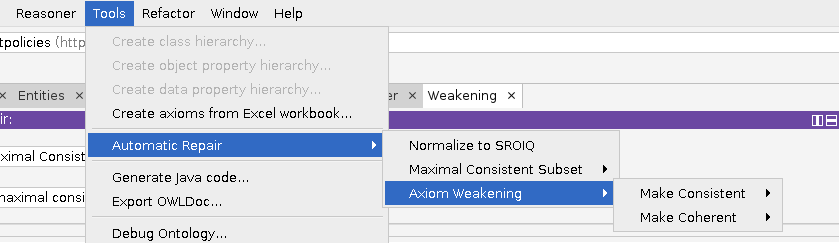
\includegraphics[width=\textwidth]{resources/protege-menu.png}
  \caption{Screenshot of the Protégé menu items added by the plugin.}
  \label{fig:protege-menu}
\end{figure}

In order to quickly apply the normalization, or automatic repair algorithms, some menu items have been added by the plugin under ``Tools''. The first menu item, ``Normalize to SROIQ'', allows the quick application of the normalization, described in \cref{owl-to-sroiq}. Then there are two different repair algorithms for which menu entries have been added. The first, used by ``Maximal Consistent Subset'' selects as the repair a randomly selected maximal consistent subset. The second, used with ``Axiom Weakening'', is based on the algorithm listed in \cref{algo:repair-weaken}. For each of these two algorithms, the user may choose between making the ontology only consistent, or making it also coherent. The repair for making the ontology coherent works analogously to the one for making the ontology consistent, except that the tests for consistency of the ontology are replaced with tests for coherence.

\begin{figure}[ht]
  \centering
  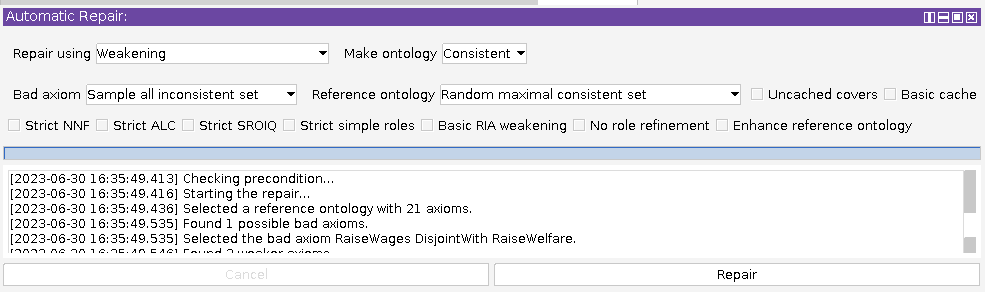
\includegraphics[width=\textwidth]{resources/protege-repair.png}
  \caption{Screenshot of the Protégé view added by the plugin, allowing for configuring and applying repairs algorithms.}
  \label{fig:protege-repair}
\end{figure}

The second method of interacting with the proposed axiom weakening repair algorithms is through a more detailed view added by the plugin. The user can select both the algorithm, e.g., by removal, using a maximally consistent set, using axiom weakening, etc., and the goal of the repair, i.e., consistency or coherence. Further, for some repair methods, options are made available. For the repair by weakening, all the flags and variations discussed in \cref{prototype} can be configured, as can be seen in \cref{fig:protege-repair}. Below the section for configuring the repair algorithm, a progress indicator and log have been placed. For long-running repairs, this is a valuable addition so that the user can see that the repair is still running. Another important feature that has been added specifically for the plugin is the ability to interrupt the repairs. To facilitate this functionality, the repair is started in a separate thread, and before every reasoner call, the implementation checks whether the thread has been interrupted, and if it has the repair is terminated by throwing an exception.

\begin{figure}[ht]
  \centering
  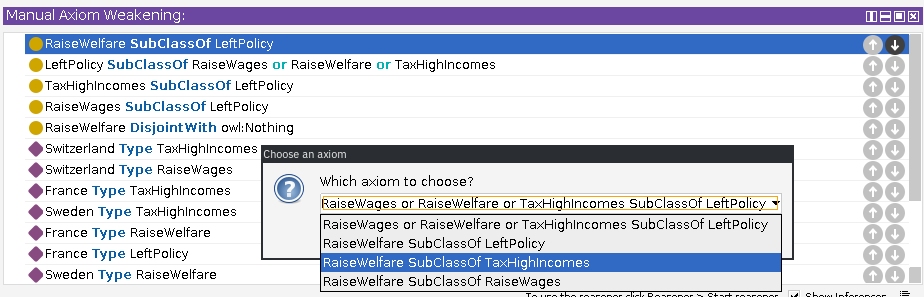
\includegraphics[width=\textwidth]{resources/protege-manual.png}
  \caption{Screenshot of the Protégé view added by the plugin, allowing for manually selecting axioms and weakening them.}
  \label{fig:protege-manual}
\end{figure}

Lastly, a view has been added that allows users to manually select how they want to weaken axioms. The view, depicted in \cref{fig:protege-manual}, shows a list of all axioms. The axioms are sorted by how frequently they appear in some minimal inconsistent subsets that are randomly sampled. The axioms that appear the most often are shown first, such that the axioms that are shown at the top of the list are the ones that would be selected by the automatic repair algorithm. The two buttons next to the axioms with the upward and downward arrow can then be used to, respectively, show weaker or stronger axioms. The user may choose one of these refined axiom to replace the original axiom.




\chapter{Experiments and Evaluation} \label{evaluation}


The evaluation of the proposed refinement and axiom weakening operator has been carried out using the implementation described in \cref{prototype} using different ontologies from BioPortal \cite{whetzel2011bioportal,bioportal}. Additionally, the pizza ontology \cite{pizzaontology} was included in the testing. The chosen ontologies are of different sizes and use a varying amount of expressive features. Some characteristics of the used ontologies are shown in \cref{table:ontologies}. On average, they contain about 289 axioms, 73 concept names, 29 role names, and 168 subconcepts. Some additional evaluation results, that did not fit into this chapter, can be found in \cref{eval-appendix}.

\begin{table}[ht]
  \scriptsize
  \begin{widepage}
    \centering
    \begin{tabular}{|lllrrrr|}
      \hline
      Abbreviation & Name & Expressivity & Axioms & Concepts & Roles & Subconcepts \\
      \hline
      admin & Nurse Administrator & $\mathcal{ALCHOIF}$ & 229 & 42 & 29 & 144 \\
      ahso & Animal Health Surveillance Ontology & $\mathcal{ALCRIF}$ & 166 & 38 & 31 & 104 \\
      cdao & Comparative Data Analysis Ontology & $\mathcal{ALCROIQ}$ & 437 & 132 & 68 & 375 \\
      cdpeo & Chronic Disease Patient Education & $\mathcal{ALCHF}$ & 422 & 41 & 31 & 170 \\
      covid19-ibo & Covid19 Impact on Banking Ontology & $\mathcal{ALCH}$ & 288 & 160 & 33 & 227 \\
      ecp & Electronic Care Plan & $\mathcal{ALCRQ}$ & 127 & 33 & 17 & 99 \\
      emo & Enzyme Mechanism Ontology & $\mathcal{ALCHQ}$ & 368 & 157 & 24 & 255 \\
      evi & Evidence Graph Ontology & $\mathcal{ALCRI}$ & 143 & 30 & 38 & 69 \\
      falls & Falls Prevention & $\mathcal{ALCH}$ & 79 & 30 & 20 & 35 \\
      fo & Fern Ontology & $\mathcal{ALCHI}$ & 59 & 31 & 4 & 46 \\
      gbm & Glioblastoma & $\mathcal{ALCIF}$ & 603 & 108 & 28 & 227 \\
      gfvo & Genomic Feature and Variation Ontology & $\mathcal{ALCH}$ & 332 & 102 & 30 & 170 \\
      koro & Knowledge Object Reference Ontology & $\mathcal{ALCHI}$ & 262 & 110 & 19 & 194 \\
      lico & Liver Case Ontology & $\mathcal{ALCHQ}$ & 366 & 93 & 36 & 230 \\
      mamo & Mathematical Modelling Ontology & $\mathcal{ALCR}$ & 229 & 107 & 3 & 154 \\
      mpio & Minimum PDDI Information Ontology & $\mathcal{ALCH}$ & 38 & 30 & 14 & 45 \\
      pizza & Pizza Ontology & $\mathcal{SHOIN}$ & 1131 & 100 & 8 & 376 \\
      provo & Provenance Ontology & $\mathcal{ALCRIN}$ & 170 & 31 & 42 & 128 \\
      qudt & Quantities, Units, Dimensions, and Types & $\mathcal{SHOIQ}$ & 293 & 74 & 73 & 177 \\
      trans & Nurse Transitional & $\mathcal{ALCROIF}$ & 244 & 44 & 22 & 123 \\
      triage & Nurse triage & $\mathcal{ALCHF}$ & 132 & 33 & 29 & 129 \\
      vio & Vaccine Investigation Ontology & $\mathcal{ALCRI}$ & 249 & 81 & 44 & 235 \\
      \hline
    \end{tabular}
  \end{widepage}
  \caption{The ontologies used for evaluation. The number of axioms, concept names, role names, and subconcepts are taken after applying preprocessing.}
  \label{table:ontologies}
\end{table}

Since the ontologies use OWL 2, the axioms and concepts do not map directly to \SROIQ. It is possible to directly apply axiom weakening to OWL 2 DL ontologies, a description of such a scheme and why it might be useful can be found in \cref{weakening-owl-2-dl}. However, in order to follow the definitions laid out in \cref{weakening-sroiq}, the OWL 2 DL axioms have been mapped to \SROIQ axioms. A detailed description of the mapping between OWL 2 DL and \SROIQ used for this evaluation can be found in \cref{owl-to-sroiq}. While some axioms have a direct mapping, others have been replaced by a set of axioms that together are equivalent. During the preprocessing, we further removed annotation axioms and axioms related to data properties and any axiom that caused any OWL 2 DL profile violation, as our weakening operator does not handle them.

Claims about runtime should generally only be used for relative comparisons and rough estimates. While they will obviously vary greatly based on hardware choices, all evaluations here have been performed on an Intel Coffee Lake system running at around 4GHz for the duration of the experiment. Unless otherwise indicated, the FaCT++ reasoner \cite{tsarkov2006fact++,factpp} was used for evaluation.

\section{Evaluating the Quality of Repairs}


In order to evaluate the proposed approach of axiom weakening, specifically for its application in the context of automatic repair of ontologies, we need a way to compare the quality of different possible repairs. As has already been discussed in \cite{troquard2018repairing}, the problem of deciding which of two possible repaired ontologies $\Omc_1$ or $\Omc_2$ is preferable is not generally well-defined. As such, this thesis will use the same measure defined for the experimental evaluation in \cite{troquard2018repairing}. The main idea is to use the size of the \emph{inferred class hierarchy} to evaluate the amount of ``information'' a repair can retain.

\begin{definition}\label{def:inf}
  The \emph{inferred class hierarchy} of an ontology $\Omc$ is given by
  \begin{align*}
    \Inf(\Omc) = \{ A \sqsubseteq B \mid A, B \in N_C \text{ and } A \sqsubseteq_\Omc B \} \enspace.
  \end{align*}
\end{definition}

To compare the relative amount of ``information'' between two ontologies, we compare them based on their differences in the inferred class hierarchy. We use for this purpose the \emph{inferable information content} (IIC) as defined in \cite{troquard2018repairing}.

\begin{definition}\label{def:iic}
  The \emph{inferable information content} of an ontology $\Omc_1$ with respect to another ontology $\Omc_2$ is given by
  \begin{align*}
    \qual(\Omc_1, \Omc_2) = \frac{| \Inf(\Omc_1) \setminus \Inf(\Omc_2) |}{|\Inf(\Omc_1) \setminus \Inf(\Omc_2)| + |\Inf(\Omc_2) \setminus \Inf(\Omc_1)|} \enspace,
  \end{align*}
  where $|X|$ is the cardinality of the set $X$.
\end{definition}

The IIC of an ontology $\Omc_1$ with respect to a second ontology $\Omc_2$, written $\qual(\Omc_1, \Omc_2)$, is a number between $0$ and $1$. A value closer to $0$ indicates that $\Omc_1$ contains more ``information'' than $\Omc_2$, while a value towards $1$ indicates the opposite. Inferred hierarchy axioms common to both ontologies do not influence the results, and if $\Omc_2$ is entailed by $\Omc_1$, then the IIC of $\Omc_1$ with respect to $\Omc_2$ is always $1$. If both $\Omc_1$ and $\Omc_2$ have some inferences that are not shared by the other ontology, the IIC will be strictly between $0$ and $1$. Note that if the cardinality of the inferred class hierarchy is larger for one ontology, then it will also be the one preferred by the IIC. Some weaknesses of this measure when it comes to evaluating repairs, like the fact that only atomic concepts are considered, have already been discussed in \cite{troquard2018repairing}. For the case of repairing \SROIQ ontologies, this is even more relevant, since the role hierarchy is entirely ignored.

The evaluation starts by first making the ontologies inconsistent. This has been achieved by repeatedly adding axioms to the ontology until it was no longer consistent. The newly added axioms were generated by strengthening randomly selected axioms of the ontology. Axioms are strengthened by applying an axiom strengthening operator, that is equivalent to the axiom weakening operator in \cref{def:weaken}, except for swapping the generalization and specialization operators and not using $\bot \sqsubseteq \top$ to remove the axiom. An axiom $\alpha'$ is stronger than another axiom $\alpha$ with respect to the ontology $\Omc$ if $\alpha' \models_\Omc \alpha$. Note that this is only a useful characterization if $\alpha \not\in \Omc$. It was ensured that the added axioms on their own were not inconsistent. After making the ontology inconsistent, it was repaired using different automatic repair algorithms. Each inconsistent ontology was repaired once with the repair algorithm using the axiom weakening operator presented in \cref{algo:repair-weaken} and once using \cref{algo:repair-remove}. As can be seen in \cref{ex:alc-weakening}, choosing a maximal consistent subset can sometimes lead to less information loss than using the weakening based algorithm. To experimentally evaluate how good weakening performs against the maximal consistent subset based repair on average, the repair was also performed by selecting a randomly sampled maximal consistent subset.

\begin{algorithm}[ht]
  \begin{algorithmic}
    \While{$\Omc$ is inconsistent}
      \State $\phi_\textnormal{bad} \gets \textsc{FindBadAxiom}(\Omc)$
      \State $\Omc \gets \Omc \setminus \{\phi_\textnormal{bad}\}$
    \EndWhile
    \State Return $\Omc$
  \end{algorithmic}
  \caption{\textsc{RepairOntologyRemove}($\Omc$)}
  \label{algo:repair-remove}
\end{algorithm}

This process, both making the ontology inconsistent and repairing it, was repeated one hundred times for each ontology, and the IIC was computed between the results of the different repair methods. The evaluation was performed using a randomly sampled maximal consistent subset as the reference ontology and by randomly sampling $16$ minimal inconsistent subsets during the selection of bad axioms in \textsc{FindBadAxiom}(\Omc). To obtain comparable results, both \textsc{RepairOntologyRemove}($\Omc$) and \textsc{RepairOntologyWeakening}($\Omc$) use the same implementation of \textsc{FindBadAxiom}($\Omc$). While the utilized OWL 2 DL reasoners are all highly optimized, they exhibit undesirable performance in some edge cases. Mostly they are fast to perform reasoning tasks like checking for consistency or entailment in the selected ontologies. However, when performance pitfalls are encountered, they may require significantly more time, making the computation required for repair unreasonably slow. For this reason, a timeout of 5 minutes was placed on the repairs execution and the outputs of runs that did not complete within this time limit were discarded and replaced by new runs. The results of these experiments are listed in \cref{table:results} and shown in \cref{fig:results-remove} and \cref{fig:results-mcs}.

\begin{table}[ht]
  \scriptsize
  \centering
  \begin{tabular}{|l|cc@{ }c|}
    \cline{2-4}
    \multicolumn{1}{l|}{} & IIC w.r.t. removal & \multicolumn{2}{c|}{IIC w.r.t. maximal consistent subset} \\
    \hline
    admin & 0.56 [0.51, 0.60] & 0.39 [0.33, 0.45] & (0.51 [0.45, 0.57]) \\
    ahso & 0.57 [0.52, 0.62] & 0.52 [0.47, 0.56] & (0.64 [0.59, 0.69]) \\
    cdao & 0.54 [0.49, 0.61] & 0.51 [0.44, 0.57] & (0.55 [0.48, 0.61]) \\
    cdpeo & 0.50 [0.47, 0.53] & 0.25 [0.20, 0.30] & (0.39 [0.33, 0.45]) \\
    covid19-ibo & 0.71 [0.67, 0.75] & 0.62 [0.58, 0.66] & (0.72 [0.68, 0.76]) \\
    ecp & 0.75 [0.70, 0.80] & 0.36 [0.30, 0.42] & (0.50 [0.44, 0.56]) \\
    emo & 0.68 [0.63, 0.72] & 0.61 [0.56, 0.65] & (0.73 [0.68, 0.77]) \\
    evi & 0.51 [0.46, 0.55] & 0.58 [0.53, 0.63] & (0.71 [0.66, 0.75]) \\
    falls & 0.75 [0.70, 0.81] & 0.50 [0.44, 0.57] & (0.60 [0.54, 0.66]) \\
    fo & 0.53 [0.48, 0.58] & 0.68 [0.63, 0.73] & (0.67 [0.62, 0.73]) \\
    gbm & 0.59 [0.54, 0.64] & 0.54 [0.49, 0.59] & (0.68 [0.63, 0.73]) \\
    gfvo & 0.53 [0.47, 0.58] & 0.54 [0.49, 0.59] & (0.71 [0.67, 0.75]) \\
    koro & 0.53 [0.48, 0.58] & 0.38 [0.32, 0.43] & (0.53 [0.47, 0.59]) \\
    lico & 0.53 [0.48, 0.59] & 0.51 [0.46, 0.57] & (0.63 [0.58, 0.68]) \\
    mamo & 0.55 [0.49, 0.61] & 0.64 [0.58, 0.69] & (0.72 [0.66, 0.77]) \\
    mpio & 0.69 [0.65, 0.74] & 0.70 [0.66, 0.75] & (0.70 [0.65, 0.74]) \\
    pizza & 0.56 [0.51, 0.62] & 0.57 [0.51, 0.63] & (0.63 [0.58, 0.69]) \\
    provo & 0.51 [0.47, 0.56] & 0.55 [0.51, 0.60] & (0.64 [0.60, 0.69]) \\
    qudt & 0.96 [0.93, 0.98] & 0.47 [0.40, 0.53] & (0.56 [0.49, 0.62]) \\
    trans & 0.56 [0.51, 0.61] & 0.41 [0.35, 0.47] & (0.51 [0.45, 0.57]) \\
    triage & 0.51 [0.46, 0.56] & 0.52 [0.47, 0.57] & (0.63 [0.57, 0.68]) \\
    vio & 0.48 [0.41, 0.54] & 0.50 [0.44, 0.57] & (0.57 [0.51, 0.63]) \\
    \hline
    Overall & 0.60 [0.58, 0.61] & 0.52 [0.50, 0.53] & (0.61 [0.60, 0.63]) \\
    \hline
  \end{tabular}
  \caption{Results of the evaluation. IIC is given as mean and 95\% confidence interval in brackets. The values in parentheses are for weakening that does not weaken the axioms in the maximal consistent subset chosen as reference ontology.}
  \label{table:results}
\end{table}

\begin{figure}[ht]
  \centering
  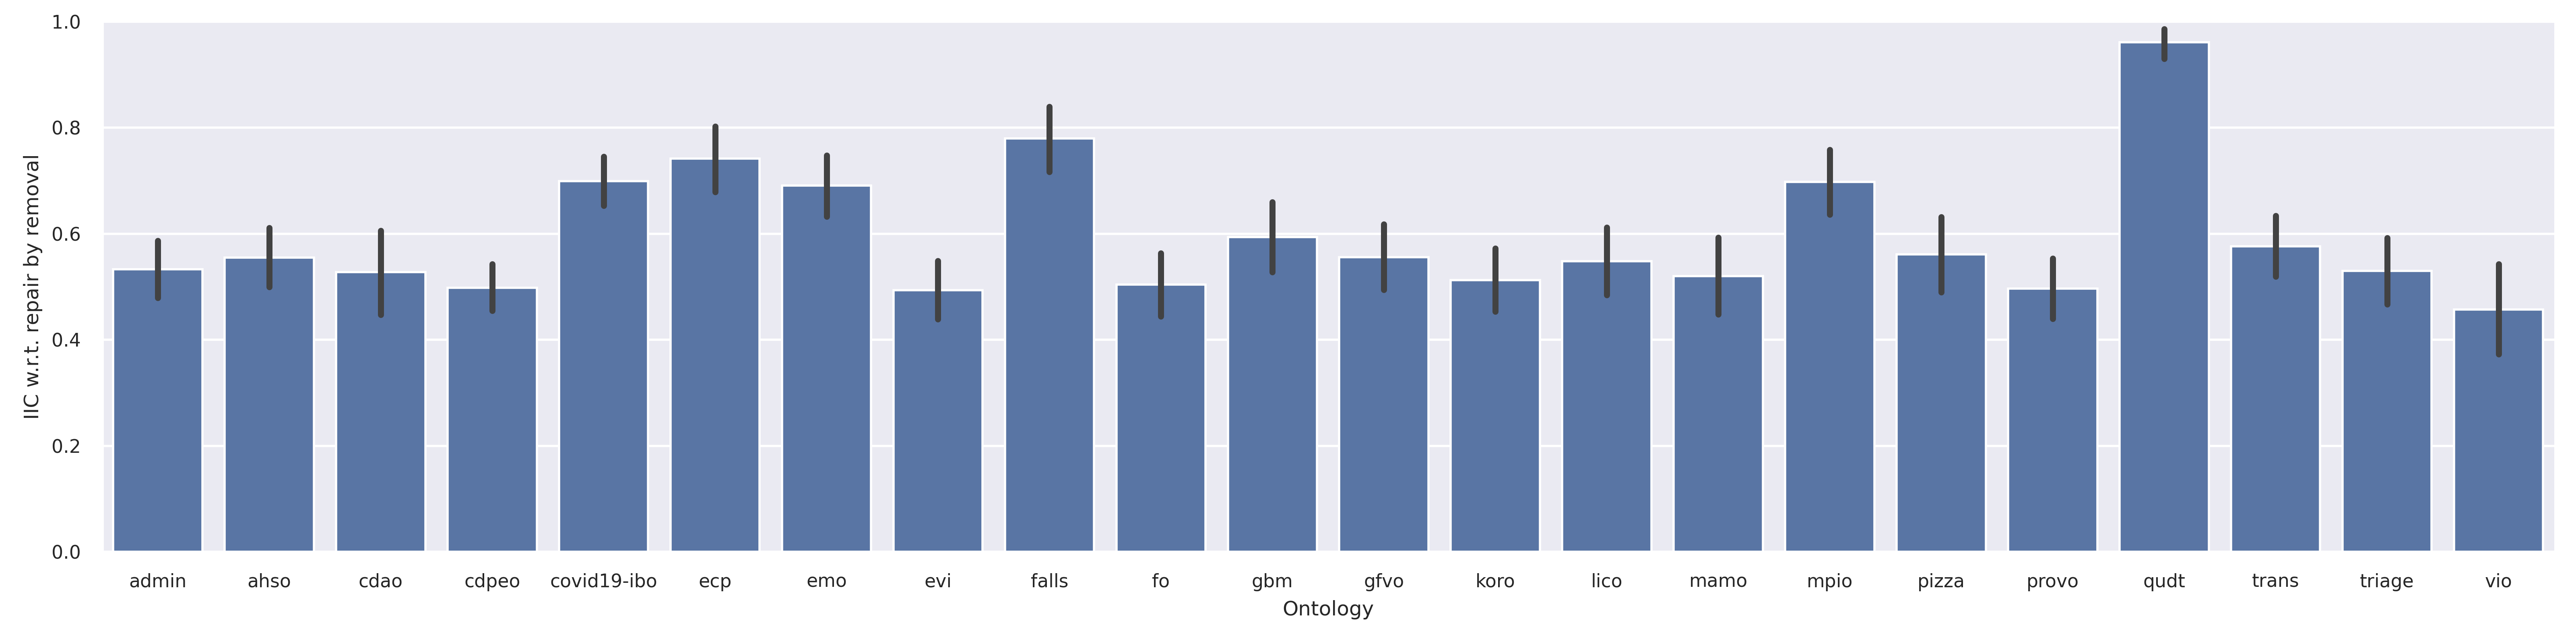
\includegraphics[width=\textwidth]{resources/iic-remove-ontology-bar.png}
  \caption{Mean IIC with respect to repair via removal per ontology. The error bars show the 95\% confidence interval.}
  \label{fig:results-remove}
\end{figure}

The results of the evaluation suggest that the repair by weakening is on average about as good or better than the repair by removal of axioms. While this supports the conclusion in \cite{troquard2018repairing} that weakening is able to retain more information than removal, the observed advantage was worse than what has been observed in \cite{troquard2018repairing}.

\begin{figure}[ht]
  \centering
  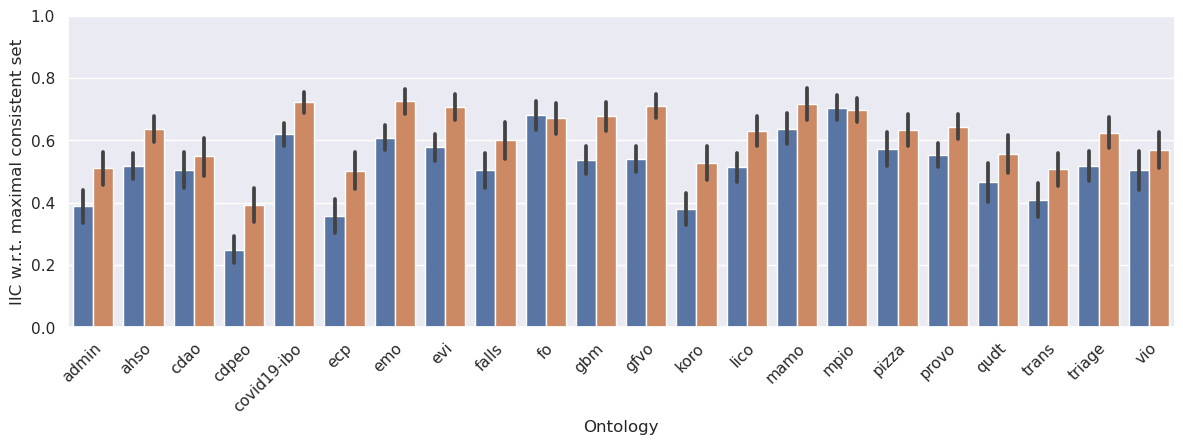
\includegraphics[width=\textwidth]{resources/iic-both-mcs-ontology-bar.png}
  \caption{Mean IIC with respect to a random maximal consistent subset. The error bars show the 95\% confidence interval. The orange bars used a variation of the repair by weakening, where axioms in the reference ontology are never weakened.}
  \label{fig:results-mcs}
\end{figure}

In contrast, it can be seen that the repair using weakening is not, in general, better than choosing a random maximal consistent subset. There are ontologies for which the repair by weakening is on average significantly worse when comparing using IIC. This is, however, a somewhat unequal comparison. We have seen in \cref{ex:alc-weakening} also a situation in which weakening performs worse when it comes to preserving information compared to choosing a maximally consistent subset. A more equal comparison, yet still not perfect since the maximal consistent subset for the reference ontology is not chosen uniformly at random, would be to a repair algorithm that starts with the reference ontology and uses weakening to add more information from the remaining axioms. This has been implemented and evaluated, and the results can be seen as the orange bars in \cref{fig:results-mcs}. Still, this result suggests that the heuristic used for selecting bad axioms is not reliable for preserving information, at least when measured using IIC. It has not been closely studied what causes the repair by weakening to significantly lose for some ontologies while being clearly preferred in others. Interestingly, there are also some cases in which the weakening based repair performs better against a random maximal consistent subset than against the repair by removal.

To overcome some weaknesses of the IIC, especially that it does not account for subsumptions between roles or complex concept expressions, tests were also carried out using an extended version of the inferred class hierarchy and IIC, adding to it subsumptions between subconcepts and roles.

\begin{definition}
  The \emph{extended inferred class hierarchy} of an ontology $\Omc$ is given by
  \begin{align*}
    \Inf^+(\Omc) ={} & \{ C \sqsubseteq D \mid C, D \in \sub(\Omc) \text{ and } C \sqsubseteq_\Omc D \} \\
    & \cup \{ R \sqsubseteq S \mid R, S \in \Lmc(N_R) \text{ and } R \sqsubseteq_\Omc S \} \enspace.
  \end{align*}
  The \emph{extended inferable information content} (IIC$^+$) of an ontology $\Omc_1$ with respect to another ontology $\Omc_2$ is given by
  \begin{align*}
    \qual^+(\Omc_1, \Omc_2) = \frac{| \Inf^+(\Omc_1) \setminus \Inf^+(\Omc_2) |}{|\Inf^+(\Omc_1) \setminus \Inf^+(\Omc_2)| + |\Inf^+(\Omc_2) \setminus \Inf^+(\Omc_1)|} \enspace,
  \end{align*}
\end{definition}

Of course, this new measure still only captures a small part of all consequences, but it should provide more accurate results when it comes to information about subconcepts and roles. When evaluating the experiment outcomes, we see that the values produced by IIC and IIC$^+$ are very similar. As may be expected, the repair by weakening is preferred slightly more strongly when using IIC$^+$. \Cref{fig:results-eiic} shows the comparison between IIC and IIC$^+$ for repair using axiom weakening w.r.t. repair by removal. The differences between IIC and IIC$^+$ are somewhat stronger when comparing against the repair using a random maximal consistent subset, but the differences are still not particularly noteworthy.

\begin{figure}[ht]
  \centering
  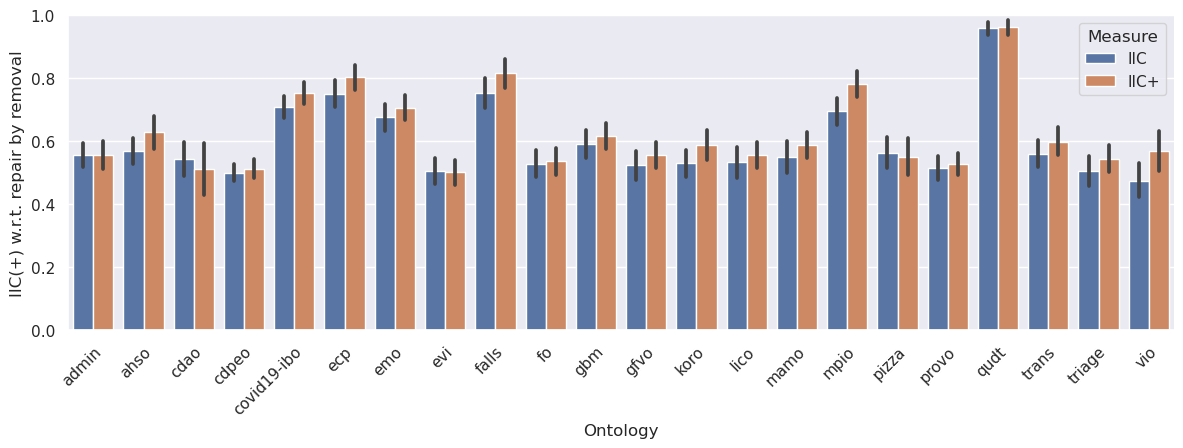
\includegraphics[width=\textwidth]{resources/iic-eiic-ontology-bar.png}
  \caption{Mean IIC and IIC$^+$ with respect to repair by removal per ontology. The error bars show the 95\% confidence interval.}
  \label{fig:results-eiic}
\end{figure}


\section{Effectiveness of Caching in Cover Computation}


As discussed in \cref{cache-impl}, to accelerate the computation of upward and downward covers, a cache was added to avoid repeated calls to the reasoner when the necessary information can already be inferred from previous computations. This section will discuss the experiments performed to evaluate the effectiveness of this cache.

Three versions of the upward and downward cover have been considered, the uncached version that calls the reasoner for every subsumption query, a version that caches only the exact queries that were already made previously, and finally the version that additionally infers some additional information from the transitivity of subsumption as listed in \cref{algo:cached-subs}. The experiment uses some of the same ontologies as have been used for the previously discussed evaluation of the repair quality. From the logical axioms of each ontology were selected, uniformly at random, one hundred groups with a fixed number of axioms. The same axioms may be selected multiple times. Each of the groups was then tested with a separate instance of the cache. The rationale behind testing with different group sizes is that the cache will obviously have a greater impact when the same cache can be reused for more cover computations. In each test run, the axiom weakening operator was applied to each axiom and the number of reasoner calls and (real) time taken were measured. The weakening operator used the complete (after preprocessing) ontology as the reference ontology. The test has further been performed using different OWL 2 DL reasoners. The final results of the evaluation can be seen in \cref{table:results-cache-calls} and are visualized in \cref{fig:results-cache-calls} and \cref{fig:results-cache-time}. Note that a logarithmic y-axis has been used for both plots.

\begin{table}[ht]
  \scriptsize
  \centering
  \begin{tabular}{|l|rrr|rrr|rrr|}
    \cline{2-10}
    \multicolumn{1}{l|}{} & \multicolumn{9}{c|}{\hspace{-4mm}Reasoner calls per weakening} \\
    \multicolumn{1}{l|}{} & \multicolumn{3}{c}{Full caching} & \multicolumn{3}{c}{Simple caching} & \multicolumn{3}{c|}{No caching} \\
    \multicolumn{1}{l|}{} & \multicolumn{1}{c}{1} & \multicolumn{1}{c}{10} & \multicolumn{1}{c}{100} & \multicolumn{1}{c}{1} & \multicolumn{1}{c}{10} & \multicolumn{1}{c}{100} & \multicolumn{1}{c}{1} & \multicolumn{1}{c}{10} & 100 \\
    \hline
    admin & 1096 & 222 & 35
      & 15138 & 2115 & 236
      & 41105 & 41288 & 41751 \\
    cdpeo & 2110 & 522 & 75
      & 13621 & 2694 & 312
      & 29051 & 28617 & 29315 \\
    emo & 2652 & 1355 & 258
      & 7781 & 2784 & 619
      & 12524 & 12134 & 12552 \\
    gbm & 3019 & 1074 & 168
      & 12572 & 3284 & 503
      & 19490 & 21330 & 20801 \\
    gfvo & 1737 & 575 & 80
      & 2828 & 1524 & 293
      & 4058 & 4104 & 4003 \\
    koro & 2006 & 591 & 80
      & 5154 & 2272 & 382
      & 7271 & 7181 & 7422 \\
    mamo &  1984 & 511 & 61
      & 3557 & 1488 & 234
      & 5060 & 5059 & 4998 \\
    \hline
    Overall & 2086 & 693 & 108
      & 8664 & 2309 & 368
      & 16937 & 17102 & 17263 \\
    \hline
  \end{tabular}
  \caption{Results of the evaluation of cache effectiveness. The mean number of reasoner calls required for a single application of the axiom weakening operator on randomly selected axioms of the ontology is given for different degrees of cache reuse. The cache is reused of one, ten, or one hundred successive operator applications.}
  \label{table:results-cache-calls}
\end{table}

\begin{figure}[ht]
  \centering
  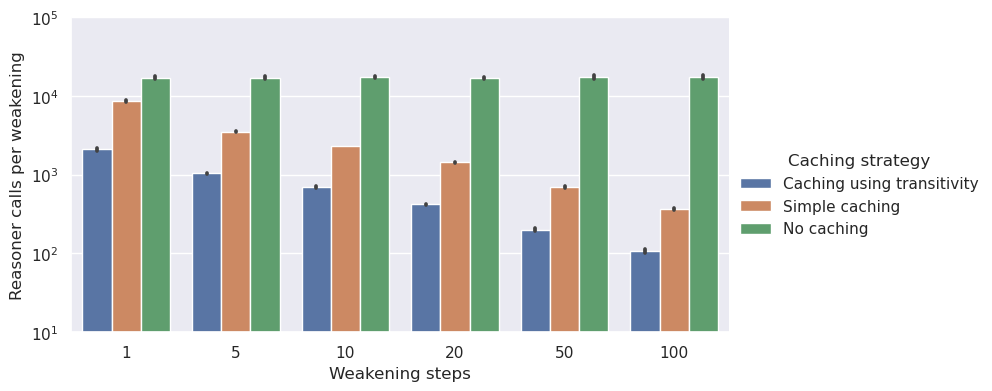
\includegraphics[width=\textwidth]{resources/calls-cache-bar.png}
  \caption{The mean number of reasoner calls needed for a single application of the axiom weakening operator, averaged over the tested ontologies.}
  \label{fig:results-cache-calls}
\end{figure}

\begin{figure}[ht]
  \centering
  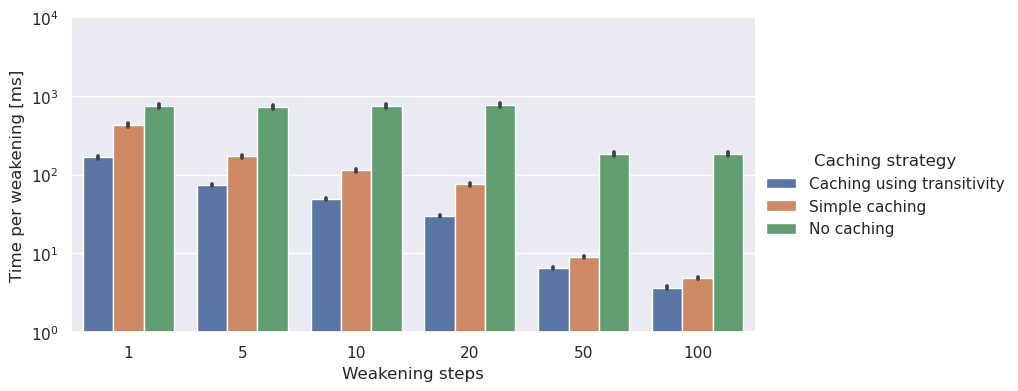
\includegraphics[width=\textwidth]{resources/time-cache-bar.png}
  \caption{Average time required per application of the axiom weakening operator with different caching strategies. The results are averaged over the tested ontologies and the reasoners FaCT++, JFact, Openllet, and HermiT.}
  \label{fig:results-cache-time}
\end{figure}

We can see clearly from the results that the cache is indeed effective at lowering both the number of reasoner calls and execution time. The simple caching method alone provides a dramatic decrease in the number of reasoner calls, especially at higher group sizes. The algorithm that can additionally exploit the transitivity of the relation performs even better, also with a smaller number of weakening steps. The difference when looking at the execution time is significantly smaller. This can likely be attributed largely to internal caching performed by the reasoners. This would also explain the observed variation when it comes to the relative improvement between different reasoners. It can be concluded that the addition of the cache greatly benefits the computation of the axiom weakening operator, especially if it can be reused for many applications of the same weakening operator.



\section{Evaluating Required Execution Time}


The performance of the axiom weakening based repair algorithm shown in \cref{algo:repair-weaken} has also been evaluated. During each repair via axiom weakening, the time taken and the number of calls to the reasoner have been registered. Additionally, the number of steps taken by the repair using axiom weakening has been observed. Also, as mentioned in \cref{eval-quality}, the repair program was put under a timeout to prevent cases where the reasoning becomes unreasonably slow. The generation of inconsistent ontologies used a similar timeout, and the same procedure was used for situations in which the reasoner ran out of memory. Timeout of the weakening procedure are shown separately from those latter cases in the results. The frequency of these cases is indicated as percentage of the overall runs finished vs started. The results of this evaluation are presented in \cref{table:results-perf} and \cref{fig:results-perf-time}.

\begin{table}[ht]
  \scriptsize
  \centering
  \begin{tabular}{|l|r@{ }lr@{ }lr@{ }lr@{ }r|}
    \cline{2-9}
    \multicolumn{1}{l|}{} & \multicolumn{2}{c}{Steps} & \multicolumn{2}{c}{Calls} & \multicolumn{2}{c}{Time [ms]} & \multicolumn{2}{c|}{Failed} \\
    \hline
    admin & 6.3 & [4.0, 9.2] & 7621 & [5601, 10118] & 9638 & [5433, 14909] & 2\% & (2\%) \\
    ahso & 2.1 & [1.7, 2.5] & 4648 & [4228, 5131] & 11469 & [8122, 15336] & 11\% & (26\%) \\
    cdao & 2.1 & [1.8, 2.5] & 16137 & [14576, 17740] & 20767 & [15204, 27269] & 19\% & (48\%) \\
    cdpeo & 1.5 & [1.3, 1.7] & 4476 & [4250, 4716] & 2050 & [1942, 2169] & 0\% & (0\%) \\
    covid19-ibo & 1.3 & [1.2, 1.5] & 14822 & [14321, 15320] & 2208 & [2126, 2296] & 4\% & (13\%) \\
    ecp & 1.3 & [1.2, 1.5] & 2020 & [1916, 2133] & 4453 & [2738, 6939] & 1\% & (14\%) \\
    emo & 1.4 & [1.3, 1.6] & 18549 & [17473, 19615] & 6582 & [4439, 9688] & 1\% & (4\%) \\
    evi & 5.0 & [3.9, 6.4] & 5955 & [4680, 7425] & 4719 & [3408, 6349] & 19\% & (64\%) \\
    falls & 1.5 & [1.3, 1.6] & 1242 & [1161, 1331] & 874 & [843, 909] & 1\% & (5\%) \\
    fo & 1.6 & [1.4, 1.8] & 1295 & [1179, 1423] & 1090 & [1025, 1164] & 38\% & (61\%) \\
    gbm & 1.5 & [1.3, 1.6] & 7608 & [7070, 8131] & 2954 & [2808, 3117] & 0\% & (0\%) \\
    gfvo & 1.8 & [1.6, 2.0] & 4167 & [3864, 4501] & 2404 & [2258, 2569] & 0\% & (0\%) \\
    koro & 1.9 & [1.7, 2.2] & 6195 & [5697, 6706] & 2456 & [2277, 2648] & 0\% & (0\%) \\
    lico & 2.6 & [2.2, 2.9] & 6638 & [6105, 7186] & 3709 & [3400, 4077] & 1\% & (22\%) \\
    mamo & 2.5 & [2.2, 2.9] & 4667 & [4228, 5128] & 2215 & [2046, 2403] & 0\% & (0\%) \\
    mpio & 2.2 & [1.8, 2.6] & 1908 & [1720, 2133] & 987 & [913, 1078] & 9\% & (30\%) \\
    pizza & 2.0 & [1.7, 2.3] & 7550 & [6723, 8419] & 26767 & [20554, 34014] & 28\% & (55\%) \\
    provo & 4.9 & [3.7, 6.3] & 6851 & [5383, 8465] & 8878 & [5962, 12348] & 4\% & (8\%) \\
    qudt & 1.1 & [1.0, 1.2] & 7044 & [6816, 7291] & 6658 & [4229, 9672] & 9\% & (38\%) \\
    trans & 3.2 & [1.8, 5.1] & 4384 & [3213, 5894] & 3684 & [1610, 6513] & 0\% & (5\%) \\
    triage & 3.2 & [2.4, 4.3] & 5166 & [4255, 6351] & 8979 & [6084, 13102] & 28\% & (51\%) \\
    vio & 2.5 & [2.1, 3.0] & 9476 & [8628, 10327] & 15199 & [10496, 20803] & 3\% & (7\%) \\
    \hline
  \end{tabular}
  \caption{Results of the evaluation with respect to performance. Number of weakening iterations, reasoner calls, and total repair time are given as sample mean, with 95\% confidence interval in brackets. The frequency of failed runs is shown as percentage of repairs by weakening that were started but not completed. In parentheses, the percentage of total failed runs, including those with timeout during generation of the inconsistent ontology. Attempts that failed were not considered for the other values.}
  \label{table:results-perf}
\end{table}

\begin{figure}[ht]
  \centering
  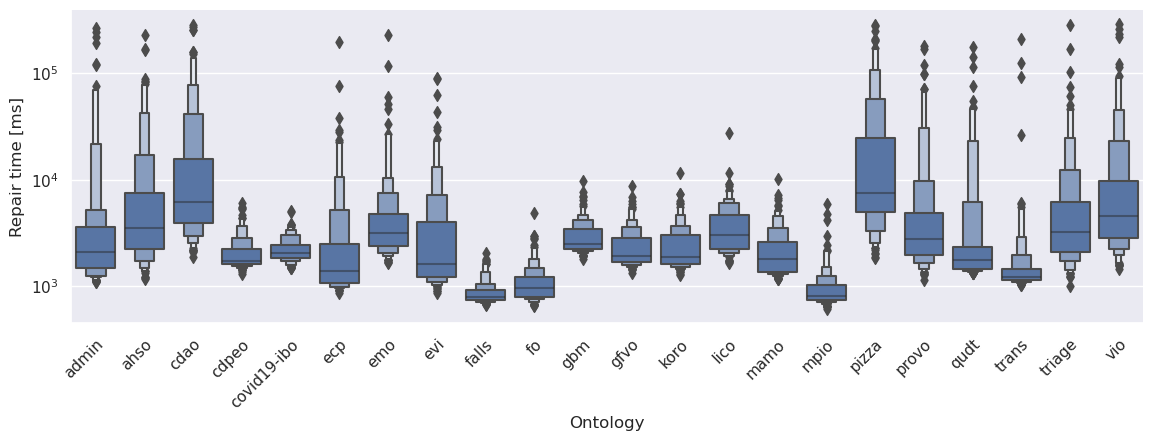
\includegraphics[width=\textwidth]{resources/time-ontology-violin.png}
  \caption{Distribution of (real) execution time required for repairing a single ontology using axiom weakening. The two darkest blue boxes represent (together) half of the samples, with the line in the middle indicating the median. Each lighter box represents half the samples of the boxes one step darker, and all remaining outliers are marked. Attempts that failed by timeout or other errors were not considered.}
  \label{fig:results-perf-time}
\end{figure}

As is visible from the results, the number of reasoner calls and the execution time can vary significantly. The execution times were generally reasonable when a run was able to complete within the time limit, with most of them completing within 2 minutes, even though the time limit was set to 5 minutes. A significant number of runs, however, were affected by the timeout or other errors. It has not been looked deeper into what causes these issues.




\chapter{Conclusion and Outlook} \label{conclusion}


This thesis has proposed refinement operators and an axiom weakening operator for all aspects of \SROIQ and shown that for repairs of inconsistent ontologies weakening can, in some cases, significantly outperform removal. The proposed approaches have been implemented both for performing the empirical evaluation and in a Protégé plugin that allows users to use the techniques described in this thesis, both for manually weakening axioms and for automatically repairing ontologies. Some ideas implemented for and discussed in the thesis, like the repair approaches focusing on finding better repairs discussed in \cref{best-repair-impl} or the relaxed RIA weakening mentioned in \cref{rbox-alternative}, have not yet been fully studied and still have to be evaluated.

Better ways for users to interact with and guide the repair process may also be studied. It can also be seen that the repair algorithm likely needs better heuristics to steer the selection of bad and weakened axioms in order to result in better repairs. This may involve also the use of domain specific information and heuristics that could steer the repair process to choose repairs that make sense also from a modelling perspective. The termination of the proposed repair algorithm should be studied, as has been done in \cite{confalonieri2020towards}. Further additions to the refinement operators may also be studied in more detail, e.g., using non-simple roles in the upward and downward covers in certain contexts. Relaxing the allowed weakening for RIAs may also be considered, and to cover also extensions to regularity conditions such as those studied in \cite{DBLP:conf/cade/Kazakov10}. Future work could further focus on finding robust measures for comparing the quality of repairs. Different applications for the axiom weakening and refinement operators, like the ones studied for concept combination in \cite{righetti2022asymmetric}, are now also able to be explored using more expressive DLs.




% I cite here all the resources I used during the creation of this thesis, for they have to be included in the bibliograhy even if not referenced directly in the text.

\nocite{troquard2018repairing}
\nocite{righetti2022asymmetric}
\nocite{kalyanpur2005debugging}
\nocite{confalonieri2020towards}
\nocite{horrocks2006even}
\nocite{ontologyutils}
\nocite{owlapi}
\nocite{factpp}
\nocite{protegepluginexamples}
\nocite{ontodebug}
\nocite{rudolph2011foundations}
\nocite{guarino1995ontologies}
\nocite{baader2018making}
\nocite{matentzoglu2016introduction}
\nocite{w3c2009owl}
\nocite{motik2012ontology}
\nocite{hitzler2012primer}
\nocite{motik2012profiles}
\nocite{bao2012reference}
\nocite{confalonieri2022irresistible}
\nocite{marques2013minimal}
\nocite{shchekotykhin2015mergexplain}
\nocite{junker2004preferred}
\nocite{kalyanpur2006repairing}
\nocite{shearer2009exploiting}
\nocite{kalyanpur2007finding}
\nocite{horridge2011owl}
\nocite{keet2021toward}
\nocite{antoniou2004semantic}
\nocite{protege5devdocs}
\nocite{reiter1987theory}
\nocite{schulz2018role}
\nocite{ji2014measuring}
\nocite{du2014practical}
\nocite{haase2007analysis}
\nocite{BaPS07}
\nocite{schlobach2003non}
\nocite{amai2016}
\nocite{du2014practical}
\nocite{LLRRS10}
\nocite{horrocks2007tableau}
\nocite{horrocks2005irresistible}
\nocite{krotzsch2010description}
\nocite{rodler2017generally}
\nocite{kazakov2012elk}
\nocite{horridge2008laconic}
\nocite{malouf2007maximal}
\nocite{schlobach2007debugging}
\nocite{kalyanpur2006axiom}


\printbibliography

\appendix

\chapter{The \texorpdfstring{$\mathcal{SROIQ}$}{SROIQ} Description Logic} \label{sroiq-appendix}


% TODO

\section{\texorpdfstring{$\SROIQ$}{SROIQ} Syntax} \label{sroiq-syntax}


The \emph{vocabulary}\footnote{There are no strict rules for how to write down different elements of the vocabulary. However, there is a convention of using PascalCase for concept names and camelCase for names referring to roles and individuals.} $N = N_I \cup N_C \cup N_R$ of a $\SROIQ$ ontology is made up of three finite disjoint sets:
\begin{itemize}
  \item The set of \emph{individual names} $N_I$ is used to refer to single elements in the domain of discourse.
  \item The set of \emph{concept names} $N_C$ is used to refer to classes that elements of the domain may be a part of.
  \item The set of \emph{role names} $N_R$ is used to refer to binary relations that may hold between the elements of the domain.
\end{itemize}
A $\SROIQ$ ontology $\Omc = \Amc \cup \Tmc \cup \Rmc$ is the union of an \emph{ABox} $\Amc$, a \emph{TBox} $\Tmc$, and a regular \emph{RBox} $\Rmc$. The elements of $\Omc$ are called axioms.

\subsection{RBox} \label{rbox}

The RBox $\Rmc$ describes the relationship between different roles in the ontology. It consists of two disjoint parts, a role hierarchy $\Rmc_h$ and a set of role assertions $\Rmc_a$.

Given the set of role names $N_R$, a \emph{role} is either the \emph{universal role} $U$ or of the form $r$ or $r^-$ for some role names $r \in N_R$, where $r^-$ is called the \emph{inverse role or} $r$. For convenience in the latter definitions, and to avoid roles like $r^{--}$, which are not valid in $\SROIQ$, we define a function $\inv$ such that $\inv(U) = U$, $\inv(r) = r^-$, and $\inv(r^-) = r$. We denote the set of all roles as $\Lmc(N_R) = N_R \cup \{ U \} \cup \{ r^- \mid r \in N_R \}$.

A \emph{role inclusion axiom} (RIA) is a statement of the form $R_1 \circ \cdots \circ R_n \sqsubseteq R$ where $R, R_1, \dots R_n \in \Lmc(N_R)$ are roles. For the case in which $n = 1$, we obtain a \emph{simple role inclusion}, which has the form $R \sqsubseteq S$ where $S$ and $R$ are role names (the case where $n > 1$ is called a \emph{complex role inclusion}). A finite set of RIAs is called a \emph{role hierarchy}, denoted $\Rmc_h$.

Roles can be partitioned into two disjoint sets, simple roles and non-simple roles. Intuitively, non-simple roles are those that are implied by the composition of two or more other roles. In order to preserve decidability, $\SROIQ$ requires that in some expressions only simple roles are used. We define the set of \emph{non-simple roles} as the smallest set such that:
\begin{itemize}
  \item the universal role $U$ is non-simple,
  \item any role $R$ that appears in a RIA of the form $S_1 \circ \cdots \circ S_n \sqsubseteq R$ where $n > 1$ is non-simple,
  \item any role $R$ that appears in a simple RIA $S \sqsubseteq R$ where $S$ is non-simple is itself non-simple, and
  \item if a role $R$ is non-simple, then $\inv(R)$ is also non-simple.
\end{itemize}
All roles which are not non-simple are \emph{simple roles}.

\begin{example}
  In the RBox $\Rmc = \{ r \circ s \sqsubseteq t, r \sqsubseteq s, t \sqsubseteq v^- \}$, the roles $t$ and $v^-$ are non-simple. $t$ is non-simple because it appears as the super role in the complex RIA $r \circ s \sqsubseteq t$. $v$ is non-simple because it appears on the right-hand side of the RIA $t \sqsubseteq v^-$, and $t$ is non-simple. Since $t$ and $v^-$ are non-simple, $t^-$ and $v$ are also non-simple. The roles $r$ and $s$ on the other hand are simple. Even though, $s$ appears as the super role in the RIA $r \sqsubseteq s$, since it is not a complex RIA and $r$ is simple, it does not affect the simplicity of $s$.
\end{example}

There is an additional restriction that is placed upon the role hierarchy in a $SROIQ$ ontology. The role hierarchy in $\SROIQ$ must be regular. A role hierarchy $\Rmc_h$ is \emph{regular} if there exists a preorder $\preceq$ (that is, a transitive and reflexive relation) on the set of roles $\Lmc(N_R)$, such that $S \prec R \iff \inv(S) \prec R$ for all roles $R$ and $S$, and all RIA in $\Rmc_h$ are $\preceq$-regular. A RIA is defined to be $\preceq$\emph{-regular} if it is of one of the following forms:
\begin{itemize}
  \item $\inv(R) \sqsubseteq R$,
  \item $R \circ R \sqsubseteq R$,
  \item $R \circ S_1 \circ \cdots \circ S_n \sqsubseteq R$,
  \item $S_1 \circ \cdots \circ S_n \circ R \sqsubseteq R$, or
  \item $S_1 \circ \cdots \circ S_n \sqsubseteq R$,
\end{itemize}
where $n > 1$ and $R$, $S$, $S_1, \cdots, S_n$ are roles such that $S \preceq R$, $S_i \preceq R$, and $R \not\preceq S_i$ for $i = 1, \dots, n$. This condition on the role hierarchy prevents cyclic definitions with RIAs that include role chains. These types of cyclic definitions could otherwise lead to undecidability of the logic.

\begin{example}
  The RBox $\Rmc = \{ r \circ s \sqsubseteq t, t \sqsubseteq v, v \sqsubseteq s \}$ is not regular. Intuitively, there exists a cyclic dependency involving a complex RIA. That is, $t$ depends on $s$ via a complex RIA, $v$ subsumes $t$, and $s$ subsumes $v$. This means, $s \preceq t$, $t \preceq v$ and $v \preceq s$ must hold. By transitivity, $t \preceq s$ must also hold. However, because the first axiom is a complex RIA, $t \not\preceq s$ must hold, causing a contradiction.
\end{example}

To make axiom weakening simpler, this definition is slightly more general than necessary. The definition of regularity presented here is more permissive than the one in \cite{horrocks2006even} in that it always allows simple roles on the left-hand side, similar to what has been described in \cite{rudolph2011foundations}. However, it is more permissive than stated in \cite{rudolph2011foundations} in that it allows for inverse roles on the right-hand side. This definition of regularity aligns more closely with the implementation of the OWL 2 DL \cite{motik2012ontology} profile checker in the OWL API \cite{horridge2011owl,owlapi}.

The set of \emph{role assertions} $\Rmc_a$ is a finite set of statements with the form $\disjoint(S_1, S_2)$ (\emph{disjointness}) where $S_1$, and $S_2$ are simple roles in $\Rmc_h$. In \cite{horrocks2006even} the authors define additionally the role assertions $\op{Sym}(R)$ (\emph{symmetry}), $\op{Asy}(S)$ (\emph{asymmetry}), $\op{Tra}(R)$ (\emph{transitivity}), $\op{Ref}(R)$ (\emph{reflexivity}), and $\op{Irr}(R)$ (\emph{irreflexivity}). These additional assertions can, however, be written using the alternative sets of axioms $\{ \inv(R) \sqsubseteq R \}$, $\{ \disjoint(R, \inv(R)) \}$, $\{ R \circ R \sqsubseteq R \}$, $\{ r' \sqsubseteq R , \top \sqsubseteq \exists r'.\self \}$, and $\{ \top \sqsubseteq \lnot \exists R.\self \}$ respectively. Note that the asymmetry assertion requires a simple role, and that $r'$ in the case of reflexivity must be a fresh role name not otherwise used in the ontology\footnote{This is necessary to allow the use of non-simple roles in a reflexivity assertion. Multiple assertions can share the same role name $r'$.}.

\subsection{TBox} \label{tbox}

The TBox $\Tmc$ describes the relationship between different concepts. In $\SROIQ$, the set of \emph{concept expressions} (or simply \emph{concepts}) given an RBox $\Rmc$ is inductively defined as the smallest set such that:
\begin{itemize}
  \item $\top$ and $\bot$ are concepts, respectively called \emph{top concept} and \emph{bottom concept},
  \item all concept names $C \in N_C$ are concept, called \emph{atomic concepts},
  \item sets of individual names $\{ a \}$ with $a \in N_I$ are concepts, called \emph{nominal concepts},
  \item if $C$ and $D$ are concepts, the $\lnot C$ (\emph{negation}), $C \sqcup D$ (\emph{union}), and $C \sqcap D$ (\emph{intersection}) are also concepts,
  \item if $C$ is a concept and $R \in \Lmc(N_R)$ a (possibly non-simple) role, then $\exists R.C$ (\emph{existential quantification}) and $\forall r.C$ (\emph{universal quantification}) are also concepts, and
  \item if $C$ is a concept, $S \in \Lmc(N_R)$ a simple role and $n \in \mathbb{N}_0$ a non-negative number, then $\exists S.\self$ (\emph{\self restriction}), $\less n S.C$ (\emph{at-most restriction}), and $\more n S.C$ (\emph{at-least restriction}) are concepts, the last two may together be referred to as \emph{qualified number restrictions}.
\end{itemize}
Given two concepts $C$ and $D$, a \emph{concept inclusion axiom} (GCI) is a statement of the form $C \sqsubseteq D$. The TBox $\Tmc$ is a finite set of GCIs.

\subsection{ABox} \label{abox}

The ABox $\Amc$ contains statements about single individuals called individual assertions. An \emph{individual assertion} has one of the following forms:
\begin{itemize}
  \item $C(a)$ (\emph{concept assertion}) for some concept $C$ and individual name $a \in N_I$,
  \item $R(a, b)$ (\emph{role assertion}) or $\lnot R(a, b)$ (\emph{negative role assertion}) for some role $R \in \Lmc(N_R)$ and individual names $a, b \in N_I$, or
  \item $a = b$ (\emph{equality}) or $a \not = b$ (\emph{inequality}) for some individual names $a \in N_I$.
\end{itemize}
An ABox $\Amc$ is a finite set of individual assertions. In $\SROIQ$ due to the inclusion of nominal concepts, all ABox axioms can be rewritten into TBox axioms.


\section{\texorpdfstring{$\SROIQ$}{SROIQ} Semantics} \label{sroiq-semantics}

\subsection{Interpretations} \label{interpretations}

The semantics of $\SROIQ$, similar to other description logics, are defined in a model-theoretic way. Therefore, a central notion in that of the interpretations. And \emph{interpretation} $I = \langle \Delta^I, \cdot^I \rangle$ consists of a set $\Delta^I$ called the \emph{domain} of $I$, and an \emph{interpretation function} $\cdot^I$. The interpretation function maps the vocabulary elements as follows:
\begin{itemize}
  \item for each individual name $a \in N_I$ to an element $a^I \in \Delta^I$ in the domain,
  \item for each concept name $C \in N_C$ to a subset $C^I \subseteq \Delta^I$ of the domain, and
  \item for each role name $r \in N_R$ to a relation $r^I \subseteq \Delta^I \times \Delta^I$ over the domain.
\end{itemize}
An interpretation maps the universal role $U$ to $U^I = \Delta^I \times \Delta^I$. We extend the interpretation function to operate over inverse roles such that  $\left(r^-\right)^I$ contains exactly those elements $\langle \delta_1, \delta_2 \rangle$ for which $\langle \delta_2, \delta_1 \rangle$ is contained in $r^I$, that is  $\left(r^-\right)^I = \{ \langle \delta_1, \delta_2 \rangle \mid \langle \delta_2, \delta_1 \rangle \in r^I \}$. Further, we define the extension of the interpretation function to complex concepts inductively as follows:
\begin{itemize}
  \item The top concept is true for every individual in the domain, therefore $\top^I = \Delta^I$.
  \item The bottom concept is true for no individual, hence $\bot^I = \empty$ where $\empty$ represents the empty set.
  \item Nominal concepts contain exactly the specified individuals, that is $\{ a \}^I = \{ a^I \}$.
  \item $\lnot C$ yields the complement of the extension of $C$, thus $(\lnot C)^I = \Delta^I \setminus C^I$.
  \item $C \sqcup D$ denotes all individuals that are in either the extension of $C$ or in that of $D$, hence $(C \sqcup D)^I = C^I \cup D^I$.
  \item $C \sqcap D$ on the other hand, denotes all elements of the domain that are in the extension of both $C$ and $D$, which can be expressed as $(C \sqcap D)^I = C^I \cap D^I$.
  \item $\exists R.C$ holds for all individuals that are connected by some element in the extension of $R$ to an individual in the extension of $C$, formally $(\exists R.C)^I = \{ \delta_1 \in \Delta^I \mid \exists \delta_2 \in \Delta^I \, . \; \langle \delta_1, \delta_2 \rangle \in R^I \, \land \, \delta_2 \in C^I  \}$.
  \item $\forall R.C$ refers to all domain elements for which all elements in the extension of $R$ connect them to elements in the extension of $C$, that is $(\forall R.C)^I = \{ \delta_1 \in \Delta^I \mid \forall \delta_2 \in \Delta^I \, . \; \langle \delta_1, \delta_2 \rangle \in R^I \to \delta_2 \in C^I \}$.
  \item $\exists R.\self$ indicates all individuals that the extension of $R$ connects to themselves, hence we let $(\exists R.\self)^I = \{ \delta \in \Delta^I \mid \langle \delta, \delta \rangle \in R^I\}$.
  \item $\less n R.C$ represents those individuals that have at most $n$ other individuals they are $R$-related to in the concept extension of $C$, that is  $(\less n R.C)^I = \{ \delta_1 \in \Delta^I \mid \left| \{ \delta_2 \in \Delta^I \mid \langle \delta_1, \delta_2 \rangle \in R^I \, \land \; \delta_2 \in C^I \} \right| \less n \}$, where $|S|$ denotes the cardinality of a set $S$.
  \item $\more n R.C$ corollary to the case above indicates those domain elements that have at least $N$ such $R$-related elements, \\$(\more n R.C)^I = \{ \delta_1 \in \Delta^I \mid \left| \{ \delta_2 \in \Delta^I \mid \langle \delta_1, \delta_2 \rangle \in R^I \, \land \; \delta_2 \in C^I \} \right| \more n \}$.
\end{itemize}

\begin{example}
  Given the interpretation $I = \langle \Delta^I, \cdot^I \rangle$ where $\Delta^I = \{ 1, 2, 3, 4, 5, 6, 7 \}$ and $P^I = \{ 2, 3, 5, 7 \}$, $E^I = \{ 2, 4, 6 \}$, $o^I = 1$, and $s^I = \{ \langle 1, 2 \rangle,\allowbreak \langle 2, 3 \rangle,\allowbreak \langle 3, 4 \rangle,\allowbreak \langle 4, 5 \rangle,\allowbreak \langle 5, 6 \rangle,\allowbreak \langle 6, 7 \rangle \}$, the extended interpretation function evaluates the following example as shown.
  \begin{align*}
    \top^I &= \{ 1, 2, 3, 4, 5, 6, 7 \} &
    (\lnot P)^I &= \{ 1, 4, 6 \} \\
    (P \cup E)^I &= \{ 2, 3, 4, 5, 6, 7 \} &
    (P \cap E)^I &= \{ 2 \} \\
    (\exists s.P)^I &= \{ 1, 2, 4, 6 \} &
    (\exists s.E \cup \exists s^-.E)^I &= \{ 1, 3, 5, 7 \} \\
    (\exists s^-.\nominal o)^I &= \{ 2 \} &
    (\exists s.\nominal o)^I &= \emptyset
  \end{align*}
\end{example}

\subsection{Satisfaction of Axioms} \label{satisfaction-of-axioms}

The purpose of the (extended) interpretation function is mainly to determine satisfaction of axioms. We define in the following when an axiom $\alpha$ is true, or holds, in a specific interpretation $I$. If this is the case, the interpretation $I$ satisfies $\alpha$, written $I \models \alpha$. If an interpretation $I$ satisfies an axiom $\alpha$, we also say that $I$ is a model of $\alpha$.
\begin{itemize}
  \item A RIA $S_1 \circ \cdots \circ S_n \sqsubseteq R$ holds in $I$ if and only if for each sequence $\delta_1, \dots, \delta_{n + 1} \in \Delta^I$ for which $\langle \delta_i , \delta_{i + 1} \rangle \in S_i^I$ for all $i = 1, \cdots, n$, also $\langle \delta_1 , \delta_n \rangle \in R^\mathcal{i}$ is satisfied. Equivalently, we can write $I \models S_1 \circ \cdots \circ S_n \sqsubseteq R \iff S_1^I \circ \cdots \circ S_n^I \subseteq R^I$ where $\circ$ denotes the composition of the relations.
  \item A role disjointness axiom $\disjoint(S, R)$ hold iff the extensions of $R$ and $S$ are disjoint, formally $I \models \disjoint(S, R) \iff S^I \cap R^I = \empty$.
  \item A GCI $C \sqsubseteq D$ is true iff the extension of $C$ is fully contained in the extension of $D$, hence $I \models C \sqsubseteq D \iff C^I \subseteq D^I$.
  \item A concept assertion $C(a)$ holds iff the individual that $a$ is mapped to by $\cdot^I$ is in the concept extension of $C$, therefore $I \models C (a) \iff a^I \in C^I$.
  \item A role assertion $R(a, b)$ holds iff the individuals denoted by the name $a$ and $b$ are connected in the extension of $R$, thus $I \models R(a, b) \iff \langle a^I, b^I \rangle \in R^I$.
  \item A negative role assertion $\lnot R(a, b)$ is true exactly then when the corresponding role assertion $R(a, b)$ is false. Equivalently, $I \models \lnot R(a, b) \iff \langle a^I, b^I \rangle \not\in R^I$.
  \item An equality assertion $a = b$ holds iff the individuals identified by $a$ and $b$ are the same element of the domain, formally written $I \models a = b \iff a^I = b^I$.
  \item Dual to the above, $a \not = b$ holds iff the names $a$ and $b$ denote different elements, accordingly $I \models a \not= b \iff a^I \not= b^I$.
\end{itemize}
We say a set of axioms holds in an interpretation $I$ iff every axiom of the set hold in $I$. Accordingly, $I$ satisfies a ontology $\Omc$, written $I \models \Omc$, iff $I$ satisfies every axiom $\alpha \in \Omc$ of the ontology, i.e., $I \models \Omc \iff \forall \alpha \in \Omc \, . \; I \models \alpha$. If $I$ satisfies $\Omc$, we say $I$ is a model of $\Omc$.

\begin{example}
  Given the interpretation $I = \langle \Delta^I, \cdot^I \rangle$ where $\Delta^I = \{ 1, 2, 3, 4, 5, 6, 7 \}$ and $P^I = \{ 2, 3, 5, 7 \}$, $E^I = \{ 2, 4, 6 \}$, $o^I = 1$, $t^I = 2$, and $s^I = \{ \langle 1, 2 \rangle,\allowbreak \langle 2, 3 \rangle,\allowbreak \langle 3, 4 \rangle,\allowbreak \langle 4, 5 \rangle,\allowbreak \langle 5, 6 \rangle,\allowbreak \langle 6, 7 \rangle \}$, the following axioms are satisfied by $I$.
  \begin{align*}
    &P \sqsubseteq \top &
    &P \sqcap \lnot (\exists s^-.\nominal o) \sqsubseteq \lnot E \\
    &P \sqcup E \sqsubseteq \lnot \nominal o &
    &\disjoint(s, s^-) \\
    &s(o, t) &
    &o \not= t
  \end{align*}
  The following axioms on the other hand are not satisfied by $I$.
  \begin{align*}
    &P \sqsubseteq \lnot E &
    &\top \sqsubseteq P \sqcup E &
    &\top \sqsubseteq \exists s.\top \\
    &s \circ s \sqsubseteq s &
    &s \sqsubseteq s^- &
    &\top \sqsubseteq{} \more 1 s.E \\
    &\lnot s(o, t) &
    &o = t &
    &s(t, o)
  \end{align*}
\end{example}

\subsection{Reasoning tasks} \label{reasoning-tasks}

In general, logic-based knowledge representation is useful for the ability to perform reasoning task on ontologies. There are a number of reasoning tasks that can be performed by a reasoner in DLs. In this section, we will have a look at three basic reasoning tasks, and how they can be reduced to each other. While there exists other reasoning task, this section will focus on \emph{ontology consistency}, \emph{axiom entailment}, and \emph{concept satisfiability}.

\subsubsection{Ontology consistency} \label{knowledge-base-satisfiability}

An ontology $\Omc$ is consistent iff there exists a model $I \models \Omc$ for $\Omc$. Otherwise, the ontology is called inconsistent. As discussed in \cref{ontology-bugs}, an inconsistent ontology can be a sign of modelling errors. An inconsistent ontology entailed every statement, and as such all information extracted from it is useless. Therefore, an inconsistent ontology is generally undesirable. Furthermore, both the task of deciding concept satisfiability and axiom entailment can be reduced to deciding ontology consistency.

\subsubsection{Axiom entailment} \label{axiom-entailment}

An axiom $\alpha$ is entailed by $\Omc$ if every model $I \models \Omc$ of the ontology also satisfies the axiom $I \models \alpha$. We also write this as $\Omc \models \alpha$ and say that $\alpha$ is a consequence of $\Omc$. Deciding axiom entailment is an important task in order to derive new information from the collected knowledge. If $\alpha$ is entailed by the empty ontology, $\alpha$ is said to be a \emph{tautology}. Further, the \emph{set of consequences} of $\Omc$ if the set of all axioms which are entailed by $\Omc$, we write $\op{Con}(\Omc) = \{ \alpha \mid \Omc \models \alpha \}.$ It is clear that the set of consequences will always be infinite, since there is an infinite number of tautologies.

The problem of axiom entailment can be reduced to determining for the satisfiability of a modified ontology. This is achieved by using an axiom $\beta$ that imposes the opposite restriction to $\alpha$, to be more precise, for all interpretations $I \models \alpha \iff I \not\models \beta$. If $\alpha$ is entailed by $\Omc$, it must hold in every model of $\Omc$, hence $\beta$ must not hold in any model. It follows that the extended ontology $\Omc \cup \{ \, \beta \, \}$ has no new model, and is therefore unsatisfiable. We can consequently solve the axiom entailment problem by testing for satisfiability of a modified ontology, if we can find such an opposing axiom for $\alpha$. For some cases in $\SROIQ$ finding such an opposite is obvious, for others the desired behaviour must be emulated with a set of axioms. \Cref{tab:entailment-reduction} shows the correspondence for every type of $\SROIQ$ axiom.
\begin{table}[ht]
  \centering
  \begin{tabular}{|l|l|}
    \hline
    $\alpha$ & $B$ \\
    \hline
    $S_1 \circ \cdots \circ S_n \sqsubseteq R$ & $S_1(a_1, a_2)$, $\dots$, $S_n(a_n, a_{n + 1})$, and $\lnot R(a_1, a_{n + 1})$ \\
    $\disjoint(S, R)$ & $S(a, b)$ and $R(a, b)$ \\
    $C \sqsubseteq D$ & $(C \sqcap \lnot D)(a)$ \\
    $C(a)$ & $\lnot C(a)$ \\
    $R(a, b)$ & $\lnot R(a, b)$ \\
    $\lnot R(a, b)$ & $R(a, b)$ \\
    $a = b$ & $a \not= b$ \\
    $a \not= b$ & $a = b$ \\
    \hline
  \end{tabular}
  \label{tab:entailment-reduction}
  \caption[Axioms substitution for reducing entailment to satisfiability]{The axioms in $B$ together have the “opposite” meaning of those in $\alpha$. This means, checking entailment of $\alpha$ with respect to $\Omc$, is equivalent to checking unsatisfiability of $\Omc \cup B$. $a$, $a_i$, and $b$ are assumed to not appear in $\Omc$.}
\end{table}

\subsubsection{Concept satisfiability} \label{concept-satisfiability}

A concept $C$ is satisfiable with respect to $\Omc$ iff there exists a model of the ontology $I \models \Omc$ such that the extension of $C$ is not empty, i.e., $C^I \not= \empty$. A concept which is not satisfiable is called unsatisfiable. Clearly, some concepts are unsatisfiable with respect to every ontology, for example $\bot$ or $A \sqcap \lnot A$. However, similar to an unsatisfiable ontology, an unsatisfiable atomic concept may be an indication of a modelling mistake.

Like axiom entailment, concept satisfiability can be reduced to ontology satisfiability. If a concept is unsatisfiable, every model $I \models \Omc$ maps the concept to the empty set, that is $C^I = \empty$. Since the other direction is trivial, we can rewrite this as $C^I \subseteq \empty$. It follows that since $\bot^I = \empty$ the every such model satisfies $I \models C \sqsubseteq \bot$, meaning $\Omc \models C \sqsubseteq \bot$. We conclude that we can test for unsatisfiability of a concept $C$ by checking for entailment of $C \sqsubseteq \bot$.




\chapter{Axiom Weakening in OWL 2 DL} \label{weakening-owl-2-dl}

Since OWL 2 DL is reducible to $\mathcal{SROIQ}$ it would be sufficient to perform this normalization and then apply the weakening as described to the resulting $\mathcal{SROIQ}$ ontology. This transformation is unproblematic in some contexts, for example if the result is only going to be used for automatic reasoning tasks. However, if the output must be further manipulated by a user of the system, the added noise introduced by the normalization may cause confuting and hinder understanding. Further, weakening OWL 2 DL ontologies directly can be seen as a heuristic, giving an indication as to which weakening might make sense from a modelling perspective.

\begin{example}
OWL has an axiom $\mathrm{DisjointClasses}(C_1, \dots, C_n)$\footnote{In the rest of this section, the OWL 2 functional syntax (cf. \cite{motik2009owl_spec}) will be used.} that allows specifying that a set of classes all are pairwise disjoint. $C_i \sqcap C_j \sqsubseteq \bot$ for all $i \not= j = 1, \dots, n$. One reasonable approach to weakening the OWL axiom is to replace any of the classes $C_i$ with a more specific class $C_i' \in \rho_\mathcal{O}(C_i)$. In contrast, after normalization, there will be $n - 1$ occurrences of $C_i$. It is unlikely, increasingly so with growing $n$, that all such occurrences will be weakened to the same concept. After weakening the normalized ontology, it is thus in general not possible to reconstruct the disjointness axiom.
\end{example}

It should be noted that working directly with OWL 2 axioms will make repairs less gentle. For some axiom types, it is not obvious how they could reasonably be weakened to another single axiom. For these kinds of axioms, removal is the only available weakening.

\begin{example}
The OWL axiom $\mathrm{EquivalentClasses}(C_1, \dots, C_n)$ can not easily be weakened. One option for weakening is removing one of the arguments. The axiom would be normalized to a set of $\mathrm{SubClassOf}$ axioms, for which both the subclass and superclasses can be modified. It is evident that this is more gentle than completely removing arguments.
\end{example}

For OWL 2 DL we must follow the same restrictions, when it comes to regularity and simplicity of roles, as for $\mathcal{SROIQ}$. The same definitions for the upward and downward covers, $\mathrm{UpCover}_\mathcal{O}$ and $\mathrm{DownCover}_\mathcal{O}$, are used. We define the refinement operator $\zeta_{\uparrow,\downarrow}$ for OWL 2 DL as follows:

\begingroup
\scriptsize
\begin{align*}
    \zeta_{\uparrow, \downarrow}(A) ={} & \uparrow (A) \qquad \text{for } A \in \mathrm{N}_c \cup \mathbf{R} \cup \{ \top , \bot \} \\
    \zeta_{\uparrow, \downarrow}(\mathrm{ObjectComplementOf}(C)) ={} & \uparrow (\mathrm{ObjectComplementOf}(C)) \\& \cup \{ \mathrm{ObjectComplementOf}(C')  \mid C' \in \zeta_{\downarrow, \uparrow} (C) \} \\
    \zeta_{\uparrow, \downarrow}(\mathrm{ObjectIntersectionOf}(C_1, \dots, C_n)) ={} & \uparrow (\mathrm{ObjectIntersectionOf}(C_1, \dots, C_n)) \\& \cup \bigcup_{i=1}^n \{\mathrm{ObjectIntersectionOf}(C_1, \dots, C_i', \dots C_n)  \mid C_i' \in \zeta_{\uparrow, \downarrow} (C_i) \} \\
    \zeta_{\uparrow, \downarrow}(\mathrm{ObjectUnionOf}(C_1, \dots, C_n)) ={} & \uparrow (\mathrm{ObjectUnionOf}(C_1, \dots, C_n)) \\& \cup \bigcup_{i=1}^n  \{ \mathrm{ObjectUnionOf}(C_1, \dots, C_i', \dots C_n)  \mid C_i' \in \zeta_{\uparrow, \downarrow} (C_i)\} \\
    \zeta_{\uparrow, \downarrow}(\mathrm{ObjectAllValuesFrom}(r, C)) ={} & \uparrow (\mathrm{ObjectAllValuesFrom}(r, C)) \\& \cup \{\mathrm{ObjectAllValuesFrom}(r', C) \mid r' \in \zeta_{\downarrow, \uparrow} (r)\} \\& \cup \{\mathrm{ObjectAllValuesFrom}(r, C') \mid C' \in \zeta_{\uparrow, \downarrow}  (C)\} \\
    \zeta_{\uparrow, \downarrow}(\mathrm{ObjectSomeValuesFrom}(r, C)) ={} & \uparrow (\mathrm{ObjectSomeValuesFrom}(r, C)) \\&  \cup \{\mathrm{ObjectSomeValuesFrom}(r', C) \mid r' \in \zeta_{\uparrow, \downarrow} (r)\} \\& \cup \{\mathrm{ObjectSomeValuesFrom}(r, C') \mid C' \in \zeta_{\uparrow, \downarrow}  (C)\} \\
    \zeta_{\uparrow, \downarrow}(\mathrm{ObjectHasSelf}(r)) ={} & \uparrow (\mathrm{ObjectHasSelf}(r)) \\&  \cup \{\mathrm{ObjectHasSelf}(r') \mid r' \in \zeta_{\uparrow, \downarrow}(r)\} \\
    \zeta_{\uparrow, \downarrow}(\mathrm{ObjectMaxCardinality}(n, r, C)) ={} & \uparrow (\mathrm{ObjectMaxCardinality}(n, r, C)) \\&  \cup \{\mathrm{ObjectMaxCardinality}(n', r, C) \mid n' \in \; \uparrow (n)\} \\&   \cup \{\mathrm{ObjectMaxCardinality}(n, r', C) \mid r' \in \zeta_{\downarrow, \uparrow}(r)\} \\&  \cup \{\mathrm{ObjectMaxCardinality}(n, r, C') \mid C' \in \zeta_{\downarrow, \uparrow} (C)\} \\
    \zeta_{\uparrow, \downarrow}(\mathrm{ObjectMinCardinality}(n, r, C)) ={} & \uparrow (\mathrm{ObjectMinCardinality}(n, r, C)) \\& \cup \{\mathrm{ObjectMinCardinality}(n', r, C) \mid n' \in \; \downarrow (n)\} \\& \cup \{\mathrm{ObjectMinCardinality}(n, r', C) \mid r' \in \zeta_{\uparrow, \downarrow}(r)\} \\& \cup \{\mathrm{ObjectMinCardinality}(n, r, C') \mid C' \in \zeta_{\uparrow, \downarrow} (C)\} \\
    \zeta_{\uparrow, \downarrow}(\mathrm{ObjectOneOf}(a_1, \dots, a_n)) ={} & \uparrow (\mathrm{ObjectOneOf}(a_1, \dots, a_n)) \\
    \text{OWL 2 concepts:} \quad & \\
    \zeta_{\uparrow, \downarrow}(\mathrm{ObjectExactCardinality}(n, r, C)) ={} & \uparrow (\mathrm{ObjectExactCardinality}(n, r, C)) \\& \cup \{ \phi_1 \sqcap \phi_2   \mid \phi_1 \in \zeta_{\uparrow, \downarrow} (\mathrm{ObjectMaxCardinality}(n, r, C)) \\ \;& \qquad \land \phi_2 \in \zeta_{\uparrow, \downarrow} (\mathrm{ObjectMinCardinality}(n, r, C)) \} \\
    \zeta_{\uparrow, \downarrow}(\mathrm{ObjectHasValue}(r, a)) ={} & \uparrow (\mathrm{ObjectHasValue}(r, a)) \\&  \cup \{\mathrm{ObjectHasValue}(r', a) \mid r' \in \zeta_{\uparrow, \downarrow} (r)\} \\&  \cup \{\mathrm{ObjectSomeValuesFrom}(r, A) \mid A \in \zeta_{\uparrow, \downarrow}  (\{a\})\}
\end{align*}
\endgroup

Using this abstract refinement operator, we build two concrete refinement operators, a generalization operator $\gamma_\mathcal{O} = \zeta_{\mathrm{UpCover}_\mathcal{O}, \mathrm{DownCover}_\mathrm{O}}$ and a specialization operator $\rho_\mathcal{O} = \zeta_{\mathrm{DownCover}_\mathcal{O}, \mathrm{UpCover}_\mathcal{O}}$. Using these generalization and specialization operators, we then define the axiom weakening operator $g_\mathcal{O}$ for OWL 2 DL axioms as follows:

\begingroup
\scriptsize
\begin{align*}
    g_\mathcal{O}(\mathrm{SubClassOf}(C, D)) =& \{\mathrm{SubClassOf}(C', D) \mid C' \in \rho_\mathcal{O} (C)\} \\& \cup \{\mathrm{SubClassOf}(C, D') \mid D' \in \gamma_\mathcal{O}  (D)\} \\
    g_\mathcal{O}(\mathrm{ClassAssertion}(C, a)) =& \{\mathrm{ClassAssertion}(C', a) \mid C' \in \gamma_\mathcal{O}  (C)\} \\
    g_\mathcal{O}(\mathrm{ObjectPropertyAssertion}(r, a)) =& \{\mathrm{ObjectPropertyAssertion}(r', a) \mid r' \in \gamma_\mathcal{O}  (r)\} \\& \cup \{ \mathrm{ObjectPropertyAssertion}(r, a), \bot \sqsubseteq \top \} \\
    g_\mathcal{O}(\mathrm{NegativeObjectPropertyAssertion}(r, a)) =& \{\mathrm{NegativeObjectPropertyAssertion}(r', a) \mid r' \in \rho_\mathcal{O}  (r)\} \\& \cup \{\mathrm{NegativeObjectPropertyAssertion}(r, a), \bot \sqsubseteq \top \} \\
    g_\mathcal{O}(\mathrm{SameIndividual}(a_1, \dots, a_n)) =& \bigcup_{i=1}^n \{ \mathrm{SameIndividual}(\{a_1, \dots, a_n\} \setminus \{a_i\}) \} \\& \cup \{ \mathrm{SameIndividual}(a_1, \dots, a_n)\} \\
    g_\mathcal{O}(\mathrm{DifferentIndividuals}(a_1, \dots, a_n)) =& \bigcup_{i=1}^n \{ \mathrm{DifferentIndividuals}(\{a_1, \dots, a_n\} \setminus \{a_i\}) \} \\& \cup \{ \mathrm{DifferentIndividuals}(a_1, \dots, a_n)\} \\
    g_\mathcal{O}(\mathrm{DisjointObjectProperties}(r_1, \dots, r_n)) ={} & \bigcup_{i=1}^n \{ \mathrm{DisjointObjectProperties}(r_1, \dots, r_i', \dots, r_n) \mid r_i' \in \rho_\mathcal{O}(r_i) \} \\
    g_\mathcal{O}(\mathrm{SubObjectPropertyOf}(s, r)) ={} & \{\mathrm{SubObjectPropertyOf}(s', r) \mid s' \in \rho_\mathcal{O} (s)\} \\& \cup \{\mathrm{SubObjectPropertyOf}(s, r') \mid r' \in \gamma_\mathcal{O}  (r) \land r \text{ is simple}\} \\& \cup \{ \bot \sqsubseteq \top \} \\
    g_\mathcal{O}(\mathrm{SubObjectPropertyOf}(\qquad \qquad \qquad \qquad &\\\mathrm{ObjectPropertyChain}(s_1, \dots, s_n), r)) ={} & \{\mathrm{SubObjectPropertyOf}( \\& \qquad \mathrm{ObjectPropertyChain}(s_1, \dots, s_i', \dots, s_n), r) \mid s_i' \in \rho_\mathcal{O} (s_i)\} \\& \cup \{\mathrm{SubObjectPropertyOf}( \\& \quad \qquad \mathrm{ObjectPropertyChain}(s_1, \dots, s_n), r)\} \\
    \text{OWL 2 axioms:} \quad & \\
    g_\mathcal{O}(\mathrm{EquivalentClasses}(C_1, \dots, C_n)) =& \bigcup_{i=1}^n \{ \mathrm{EquivalentClasses}(\{C_1, \dots, C_n\} \setminus \{C_i\}) \} \\& \cup \{ \mathrm{EquivalentClasses}(C_1, \dots, C_n) \} \\
    g_\mathcal{O}(\mathrm{DisjointClasses}(C_1, \dots, C_n)) =& \bigcup_{i=1}^n \{ \mathrm{DisjointClasses}(C_1, \dots, C_i', \dots, C_n) \mid C_i' \in \rho_\mathcal{O}(C_i) \} \\
    g_\mathcal{O}(\mathrm{DisjointUnion}(D, C_1, \dots, C_n)) =& \{ \mathrm{DisjointUnion}(D, C_1, \dots, C_n), \bot \sqsubseteq \top \} \\
    g_\mathcal{O}(\mathrm{EquivalentObjectProperties}(r_1, \dots, r_n)) =& \bigcup_{i=1}^n \{ \mathrm{EquivalentObjectProperties}(\{r_1, \dots, r_n\} \setminus \{r_i\}) \} \\& \cup \{ \mathrm{EquivalentObjectProperties}(r_1, \dots, r_n) \} \\
    g_\mathcal{O}(\mathrm{InverseObjectProperties}(s, r)) ={} & \{ \mathrm{InverseObjectProperties}(s, r), \bot \sqsubseteq \top \} \\
    g_\mathcal{O}(\mathrm{FunctionalObjectProperty}(r)) ={} & \{ \mathrm{FunctionalObjectProperty}(r), \bot \sqsubseteq \top \} \\
    g_\mathcal{O}(\mathrm{InverseFunctionalObjectProperty}(r)) ={} & \{ \mathrm{InverseFunctionalObjectPro}(r), \bot \sqsubseteq \top \} \\
    g_\mathcal{O}(\mathrm{SymmetricObjectProperty}(r)) ={} & \{ \mathrm{SymmetricObjectProperty}(r), \bot \sqsubseteq \top \} \\
    g_\mathcal{O}(\mathrm{AsymmetricObjectProperty}(r)) ={} & \{ \mathrm{AsymmetricObjectProperty}(r), \bot \sqsubseteq \top \} \\
    g_\mathcal{O}(\mathrm{TransitiveObjectProperty}(r)) ={} & \{ \mathrm{TransitiveObjectProperty}(r), \bot \sqsubseteq \top \} \\
    g_\mathcal{O}(\mathrm{ReflexiveObjectProperty}(r)) ={} & \{ \mathrm{ReflexiveObjectProperty}(r), \bot \sqsubseteq \top \} \\
    g_\mathcal{O}(\mathrm{IrreflexiveObjectProperty}(r)) ={} & \{ \mathrm{IrreflexiveObjectProperty}(r), \bot \sqsubseteq \top \} \\
    g_\mathcal{O}(\mathrm{ObjectPropertyDomain}(r, C)) ={} & \{\mathrm{ObjectPropertyDomain}(r, C') \mid C' \in \gamma_\mathcal{O}  (C)\} \\
    g_\mathcal{O}(\mathrm{ObjectPropertyRange}(r, C)) ={} & \{\mathrm{ObjectPropertyRange}(r, C') \mid C' \in \gamma_\mathcal{O}  (C)\}
\end{align*}
\endgroup


\chapter{Mapping between OWL 2 DL and \SROIQ} \label{owl-to-sroiq}


% TODO



\chapter{User Guide: Java Axiom Weakening Library} \label{guide-prototype}


This section will explain how to use the prototype that has been implemented for the evaluation. There are two main ways in which someone may want to use the implementation. First, as a Java library for axiom weakening. This use case will only be discussed briefly. Second, the prototype may be used to apply the axiom weakening based repair to OWL ontology files using the implemented applications.

\section{Building the Software}

The prototype is implemented in Java and will require at least Java version 17. The Maven tool has been used for dependency management. Both Maven and a Java 17 JDK must be installed for building this project. To download and build the project, the following code can be executed. After building, the packaged JAR files will be located in \inlinecode{target/}. There will be two different packages, one containing only the code in the project named \inlinecode{ontologyutils-X.X.X.jar}, and one containing also all required dependencies named \inlinecode{shaded-ontologyutils-X.X.X.jar}.

\begin{lstlisting}
git clone https://github.com/rolandbernard/ontologyutils
cp ontologyutils
mvn clean compile package
\end{lstlisting}

If you would rather use the pre-packaged jar files, those are also available in the GitHub repository at \url{https://github.com/rolandbernard/ontologyutils/releases}. Note that the releases may be out of date with the master branch of the repository.

\section{Use as a Library}

Since the project is implemented as a Maven project, it is possible to use it as a dependency for another Maven project. To add the library as a dependency, if you have built the project yourself and run \inlinecode{mvn install}, it is sufficient to add the following to your \inlinecode{pom.xml} file. 

\begin{lstlisting}
<dependency>
  <groupId>ontologyutils</groupId>
  <artifactId>ontologyutils</artifactId>
  <version>0.1.0</version>
</dependency>
\end{lstlisting}

There is also the possibility to let Maven handle the installation from the repository by adding the following configuration to the \inlinecode{pom.xml} file. This will add the GitHub Maven repository and download the dependency from the ones available at \url{https://github.com/rolandbernard?tab=packages&repo_name=ontologyutils}.

\begin{lstlisting}
<repositories>
    <repository>
        <id>github</id>
        <url>https://maven.pkg.github.com/rolandbernard/*</url>
    </repository>
</repositories>
\end{lstlisting}

Javadoc comments are included for most classes and methods, so it should be rather easy to understand the structure of the project.

\section{Using the Applications}

To simply use the applications that were also used for the evaluation in this thesis, use the JAR file produced during building. The packaged output at \inlinecode{target/shaded-ontologyutils-X.X.X.jar} will include all the necessary dependencies. From there it is enough to run the JAR file using a command if the form \inlinecode{java -cp <jar-file> www.ontologyutils.apps.<app-class> [argument ...]}, where \inlinecode{<jar-file>} should be replaced with the path to the JAR package and \inlinecode{<app-class>} should be replaced with one of the following.

\begin{itemize}
    \item \inlinecode{BenchCache} \enspace Is a utility application used for the evaluation of the cache effectiveness. It is not intended to be used by an end user.
    \item \inlinecode{Benchmark} \enspace Is another utility for benchmarking the performance of the axiom weakening implementation.
    \item \inlinecode{CheckConsistency} \enspace Is an application to test the consistency of an ontology, possibly using multiple different reasoner implementations.
    \item \inlinecode{ClassifyOntology} \enspace Can be used to determine whether an ontology fits into a certain OWL 2 profile. Further, it also shows how expressive the description logic features used are.
    \item \inlinecode{CleanupOntology} \enspace This application was used for the evaluation to apply normalization and remove axioms violating the OWL 2 DL profile.
    \item \inlinecode{EvaluateRepairs} \enspace Can be used to compute the size of the inferred class hierarchy and the IIC between different ontologies.
    \item \inlinecode{MakeInconsistent} \enspace Can be used to make a consistent ontology inconsistent by adding stronger versions of the axioms until they cause inconsistency.
    \item \inlinecode{RepairMcs} \enspace Can be used to repair an ontology using a randomly sampled maximal consistent subset.
    \item \inlinecode{RepairRemoval} \enspace Enables the repair of an ontology using the repair algorithm using removal.
    \item \inlinecode{RepairWeakening} \enspace Enables the repair of an ontology using the repair algorithm using axiom weakening.
    \item \inlinecode{ShowOntology} \enspace Is a simple application that prints all the axioms in the ontology.
\end{itemize}

To get specific information about how to use an application, simply use the \inlinecode{--help} argument. For example, the following is the help output for the \inlinecode{RepairWeakening} application.

\begin{lstlisting}
Usage: www.ontologyutils.apps.RepairWeakening [options] <file>
Options:
  -h --help                print this help information and quit
  -o --output=<file>       the file to write the result to
  -n --normalize           normalize the ontology before repair
  --normalize-nnf          normalize the ontology to NNF before repair
  -R --no-repair           no not perform repair
  -v --verbose             print more information
  -V --extra-verbose       print even more information
  --limit=<integer>        number of repairs to generate
  --no-limit=<integer>     only stop once all repairs have been generated
  --reasoner={fact++|hermit|jfact|openllet}
                           the reasoner to use
  --coherence              make the ontology coherent
  --fast                   use fast methods for selection
  --ref-ontology={any|intersect|intersect-of-some|largest|random|random-of-some}
                           method for reference ontology selection
  --bad-axiom={largest-mcs|least-mcs|most-mus|one-mcs|one-mus|random|some-mcs|some-mus}
                           method for bad axiom selection
  --strict-nnf             accept and produce only NNF axioms
  --strict-alc             accept and produce only ALC axioms
  --strict-sroiq           accept and produce only SROIQ axioms
  --strict-simple-roles    use only simple roles in upward and downward covers
  --uncached               do not use any caches for the covers
  --basic-cache            use only a basic cache
  --strict-owl2            does not produce intersection and union with a single operand
  --simple-ria-weakening   do not use the more advanced RIA weakening
  --no-role-refinement     do not refine roles in any context
  --enhance-ref            keep the reference ontology as static axioms in the output
  --preset={bernard2023|confalonieri2020|troquard2018}
                           configuration approximating description in papers
  <file>                   the file containing the original ontology
\end{lstlisting}

To repair the ontology in the file \inlinecode{inconsistent.owl} using the axiom weakening based repair algorithm, and write the repaired ontology to \inlinecode{consistent.owl}, for example, using the configuration used for the evaluation in this thesis, one would execute the following command.

\begin{lstlisting}
java -cp target/shaded-ontologyutils-0.1.0.jar www.ontologyutils.apps.RepairWeakening inconsistent.owl -o consistent.owl
\end{lstlisting}


\chapter{User Guide: Protégé Plugin} \label{guide-plugin}


This section will cover how to install and use the Protégé plugin developed to allow using the techniques presented in the thesis.

\section{Installation}

The Protégé plugin can either be compiled and packaged from source, or is available at \url{https://github.com/rolandbernard/protege-weakening/releases}. If you desire to compile the plugin from source, you will need a Java 11 JDK and the Maven tool. If you have both of these, you can execute the following command to package the plugin, and thereafter, find the bundled JAR file in \inlinecode{target/protege-weakening-X.X.X.jar}.

\begin{lstlisting}
git clone https://github.com/rolandbernard/protege-weakening
cp protege-weakening
mvn clean compile package
\end{lstlisting}

The JAR file of the plugin must be placed into the plugin folder of Protégé. The location of this folder will vary depending on the platform and configuration of Protégé. In a Linux based environment, for example, it will most likely be located in \inlinecode{\$HOME/.Protege/plugins/}. After copying the JAR file of the plugin into this folder, the plugin will automatically be loaded and initialized the next time Protégé is started. Note that the plugin will require at least Java 11 and Protégé version 5.6.1. The plugin may work for some older Protégé versions, but this has not been tested.

\section{Using the Menu}

\begin{figure}[htbp]
  \centering
  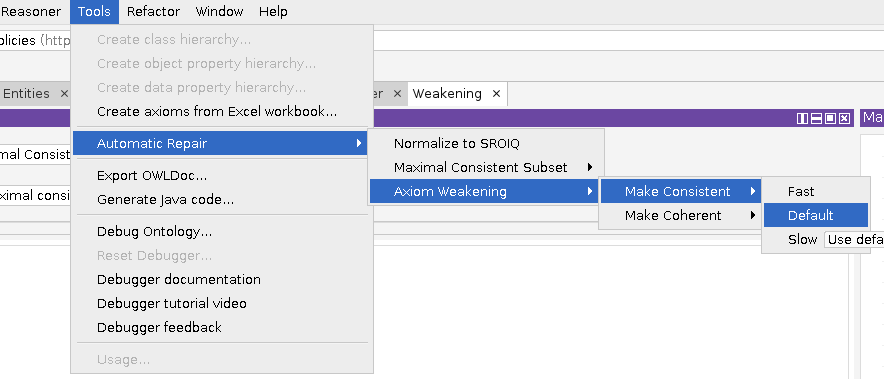
\includegraphics[width=\textwidth]{resources/protege-guide-menu.png}
  \caption{The menu items added by the plugin in Protégé.}
\end{figure}

The easiest way to use the plugin is by using the added menu items in the ``Tools'' section of the top menu. There are three main menu items. The ``Normalize to SROIQ'' entry will execute the normalization of the ontology that has also been used for the evaluation in the thesis. This will transform all OWL 2 axioms into axioms that more directly correspond to \SROIQ. Note that doing this is not required for starting the repair algorithms, since the axiom weakening operator implemented in the plugin has been extended to handle all OWL 2 axioms.

The next two menu items are for applying two different automatic repair algorithms. For each of them, there is the option to select between making the ontology only consistent, or making it also coherent. Note that when selecting coherence as the goal, the repairs will likely be slower, also because computing coherence is more expensive, at least using the way it is implemented for the plugin. The first repair method, used with the item ``Maximal Consistent Subset'', will select some randomly sampled maximal consistent subset. The second repair method, ``Axiom Weakening'', on the other hand, uses the axiom weakening based repair algorithm. Note that for each of these algorithms, there is also a choice between ``Fast'', ``Default'', or ``Slow''. These are some presets that make different choices of how to configure the repair algorithms. As their name suggests, they mainly consider options that have an impact on the performance of the algorithm. To have greater control over these parameters, use the automatic repair view.

\section{Using the Automatic Repair View}

\begin{figure}[htbp]
  \centering
  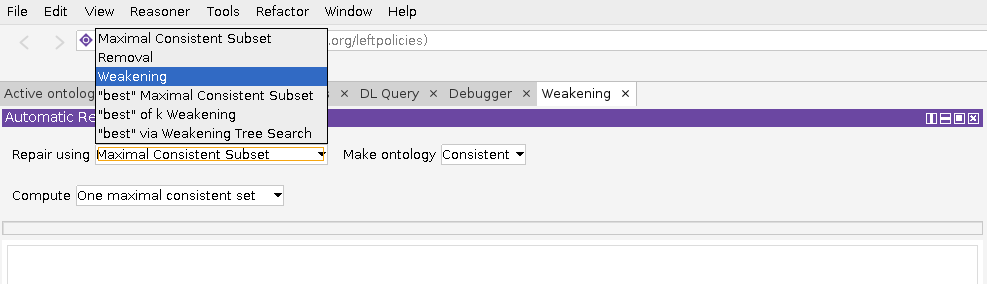
\includegraphics[width=\textwidth]{resources/protege-guide-algorithms.png}
  \caption{The automatic repair view added to Protégé. Showing the selection of possible algorithms.}
\end{figure}

The automatic repair view can be accessed in ``Window'' > ``Views'' > ``Ontology views'' > ``Automatic Repair''. It allows the user to select between a number of different repair algorithms. The one using axioms weakening and the one using a maximal consistent subset are the same as the ones accessible through the menu. The repair by removal is similar to the axiom weakening based repair, but the axioms are always removed instead of being weakened. The remaining three algorithms are all trying to optimize the IIC of the resulting repairs. For ``'best' Maximal Consistent Subset'' and ``best' of k Weakening'' this is done by sampling repairs using, respectively, maximal consistent subsets or axiom weakening, and then selecting from those the one that has the largest inferred call hierarchy. The algorithm used when selection ``'best' via Weakening Tree Search'', on the other hand, uses a Monte-Carlo tree search based approach to find the ontology with the largest inferred class hierarchy. Note that these last three repairs are significantly slower, both because they need to compute multiple repairs, and because they have to compute the inferred class hierarchy for each of them.

\begin{figure}[htbp]
  \centering
  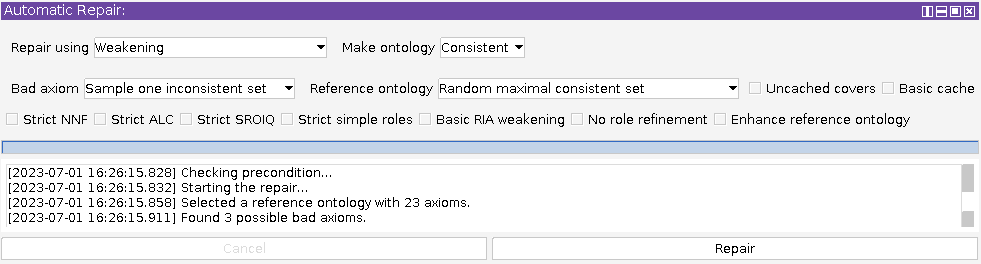
\includegraphics[width=\textwidth]{resources/protege-guide-config.png}
  \caption{The automatic repair view added to Protégé. Showing the different parameters that can be configured for the axiom weakening based repair method.}
  \label{fig:protege-guide-config}
\end{figure}

For each of these repair algorithms, a number of different configuration option are made available to the user. \Cref{fig:protege-guide-config} shows the parameters that may be configured for the axiom weakening based repair algorithm. This includes different approaches for selecting reference ontologies and bad axioms. There are some options that allow using stricter checks, such as only allowing negation normal form, or only \ALC axioms and concepts. Further, there are some parameters that simplify the refinement of roles and one that chooses to not modify the axioms of the reference ontology.

To start the repair, use the ``Repair'' button at the bottom of the view. Some information about the running repair will be printed to the text output. While the repair is running, it can be interrupted by using the ``Cancel'' button that will become enabled whenever a repair is running. If a repair is cancelled, no change will be made to the ontology in Protégé. As soon as the repair completes, on the other hand, the changes will be applied to the active ontology.

\section{Using the Manual Weakening View}

\begin{figure}[htbp]
  \centering
  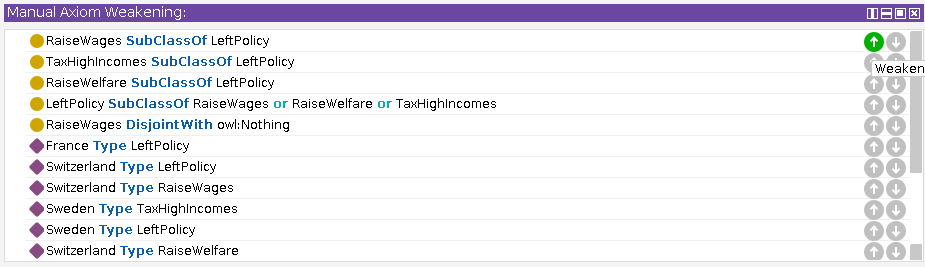
\includegraphics[width=\textwidth]{resources/protege-guide-list.png}
  \caption{The manual axiom weakening list added to Protégé. Use the buttons next to the axioms to weaken or strengthen the axioms.}
\end{figure}

The last view implemented by the plugin, and accessible under ``Window'' > ``Views'' > ``Ontology views'' > ``Manual Axiom Weakening'', allows for manually selecting which axioms to refine. The view shows a list of all axioms in the currently active ontology. The axioms are sorted by how frequently they appear in randomly sampled minimal inconsistent subsets. The axioms appearing the most often are shown at the top of the list. This means, that the axioms that would be chosen for weakening by the automatic repair algorithms are the ones appearing first in the list. Next to each axiom are two buttons, one with an upwards and one with a downwards arrow. These can be used to, respectively, compute the axiom weakenings or axiom strengthening operator for that axiom.

\begin{figure}[htbp]
  \centering
  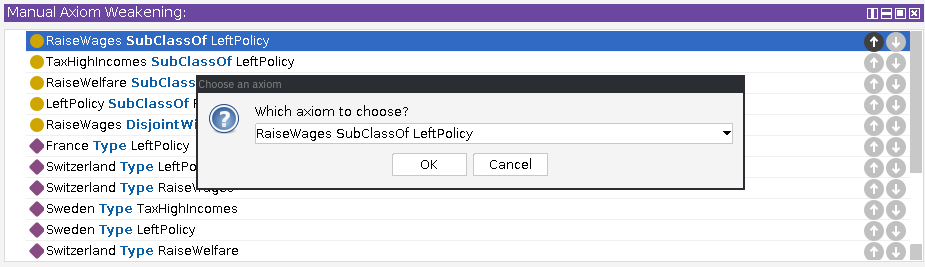
\includegraphics[width=\textwidth]{resources/protege-guide-replace.png}
  \caption{The selection of which refined axiom to use for replacing the original axiom, for the manual axiom weakening list added to Protégé.}
\end{figure}

Pressing one of these buttons will bring up a selection dialogue showing the results of the axiom weakening or strengthening operator. The user may then select from the presented choices one axiom and click ``Ok''. The original axiom will be removed from the ontology and replaced with the selected axiom. If the ``Cancel'' button is used on the other hand, no change will be made to the ontology.



\end{document}
